\documentclass[12pt]{article}
\usepackage{a4wide}
\usepackage{amsmath,amssymb}
\usepackage{bm}
\usepackage[colorlinks]{hyperref}
\usepackage{graphicx}

\usepackage{algorithm}
\usepackage{algorithmic}

\usepackage{float}
\usepackage{bbold}
\usepackage{comment}
\usepackage{mathtools}


%\usepackage{caption,refstyle}

% Package diagramme Processus de Production de la GS
\usepackage{tikz}
\usetikzlibrary{positioning, shadows}


\usepackage[french]{babel}
\usepackage[T1]{fontenc}
\usepackage{lmodern}

\DeclareUnicodeCharacter{2009}{\,} 
\usepackage[standard]{ntheorem}



\usepackage{tikz}
\usepackage{graphicx}
\usetikzlibrary{positioning, arrows.meta}
\usepackage{amsmath}
\usepackage{pdfpages}
\usepackage{adjustbox}




\begin{document}

\begin{titlepage}
\title{}
\author{Congo Job
\\ Stage Master 2 \\
 IRMA, Université de Strasbourg, France}
\date{ }

\begin{figure}[b!]
\centering
\vfill

\includegraphics[scale=0.16]{Images/Presentation/logo-unistra.pdf}
\hspace{0.5 cm}

\includegraphics[scale=0.16]{Images/Presentation/logo-Fonderie.pdf}
\hspace{0.5 cm}

\includegraphics[scale=0.16]{Images/Presentation/logoCSMI.pdf}
\end{figure}
\end{titlepage}


\maketitle
\thispagestyle{empty}


\newpage

\tableofcontents

\newpage

% \section{Présentation de l'entreprise : Fonderie de Niederbronn}
\section{Contexte }


%  Mettre une introduction générale ici soit en section soit sans!!!
\subsection{Introduction rapide}


% Dire quelque généralité

La fonderie est un secteur qui fabrique des pièces moulées en métal. 
Elle couvre une variété d’alliages, du fer à l’aluminium en passant 
par le cuivre.

Dans ce document, nous avons le rapport de stage qui a eu lieu dans l'équipe
d'Informatique de la Fonderie de Niederbronn. Il s'est déroulé sur
une période de quatre mois, entre le 11 mars et le 26 juillet 2024. 
On retrouvera tous les documents du stage dans ce 
lien : \url{https://github.com/master-csmi/2022-stage-job-br}. 


% Presenter rapidement le plan du rapport
Le présent rapport couvre les éléments suivants : la présentation de 
la fonderie de Niederbronn, la description du processus 
de production et de l'objectif du stage, l'étude statistique,  

mandat du stage la méthodologie utilisée durant le stage, et les résultats du stage. En
fin une conclusion boucle ce rapport de stage.



\subsection{Présentation de la Fonderie de Niederbronn}

%---- presenter la Fonderie,...

La Fonderie de Niederbronn, fondée en 1769, est un partenaire clé dans la production de pièces 
en fonte. Grâce à son expérience et son savoir-faire, l'entreprise produit des pièces en fonte 
à graphite lamellaire (GJL) et à graphite sphéroïdal (GJS) pour une clientèle industrielle variée,
aussi bien en France qu'à l'international. L’usine est située au Nord-Est de la France 
à Niederbronn près de Strasbourg.



\subsubsection*{Capacités et Installations de Production}
\textbf{Moyens de Fusion:}
\begin{itemize}
    \item 2 fours Junker 5T d'une puissance de 4MW.
\end{itemize}

\textbf{Lignes de Moulage:}
\begin{itemize}
    \item \textbf{DISAMATIC 270} : Coulée automatique verticale pour des pièces jusqu'à 950 x 700 mm et un poids maximum de 40 kg.
    \item \textbf{HWS} : Coulée automatique horizontale pour des pièces de dimensions jusqu'à 1600 x 1400 mm et un poids maximum de 600 kg.
\end{itemize}

\textbf{Moyens de Noyautage:}
\begin{itemize}
    \item 5 machines à noyer avec une capacité de production allant de 1 à 100 litres et des noyaux jusqu'à 300 kg.
\end{itemize}

\textbf{Moyens de Peinture:}
\begin{itemize}
    \item 2 lignes de peinture liquide pouvant traiter des pièces jusqu'à 500 kg. Peintures disponibles : primaire d'accrochage, peinture résistante aux brouillards salins de 300h, haute température (600°C).
\end{itemize}

\textbf{Moyens d'Usinage:}
\begin{itemize}
    \item Tours et centres d'usinage CNC avec des capacités variées pour des pièces de grandes dimensions (jusqu'à 1200 x 1000 x 600 mm).
\end{itemize}

\subsubsection*{Contrôle Qualité}
La Fonderie de Niederbronn attache une grande importance à la qualité de ses produits, mise en œuvre à travers divers contrôles :
\begin{itemize}
    \item \textbf{Dimensionnel:} Utilisation de bras FARO et scan 3D.
    \item \textbf{Non Destructif:} Banc de magnétoscopie et contrôle par ultrasons.
    \item \textbf{Caractéristiques Mécaniques:} Traction, contrôle de dureté, résilience.
    \item \textbf{Métallurgiques:} Spectrométrie et micrographie.
\end{itemize}

\subsubsection*{Secteurs d'Activité}
\sloppy
La Fonderie de Niederbronn sert plusieurs secteurs industriels et domestiques, 
en fournissant des pièces spécifiques adaptées aux besoins de chaque domaine.
\begin{itemize}
    \item \textbf{Usage Industriel :} Le Machinisme Agricole, les Machines du BTP, les Pièces Hydrauliques,...
    \item \textbf{Usage Domestique :} Les Corps de Chaudière et Radiateurs, les Poêles et Inserts de Cheminée,...
\end{itemize}

\subsubsection*{Chiffres Clés et Ressources Humaines}
\begin{itemize}
    \item \textbf{Nombre de Collaborateurs:} 170.
    \item \textbf{Capacité de Fusion:} 20 000 tonnes par an.
    \item \textbf{Chiffre d'Affaires:} 23 millions d'euros pour l'exercice 2023.
\end{itemize}


% - Mettre les 2 images fonderie vue de haut et une autre en vue de face.
\sloppy
Cette présentation met en lumière l'expertise, les capacités de production,
et l'engagement qualité de la Fonderie de Niederbronn, faisant d'elle un acteur 
incontournable dans le secteur de la fonderie.


\begin{figure}[H]
    \centering
    \vfill
    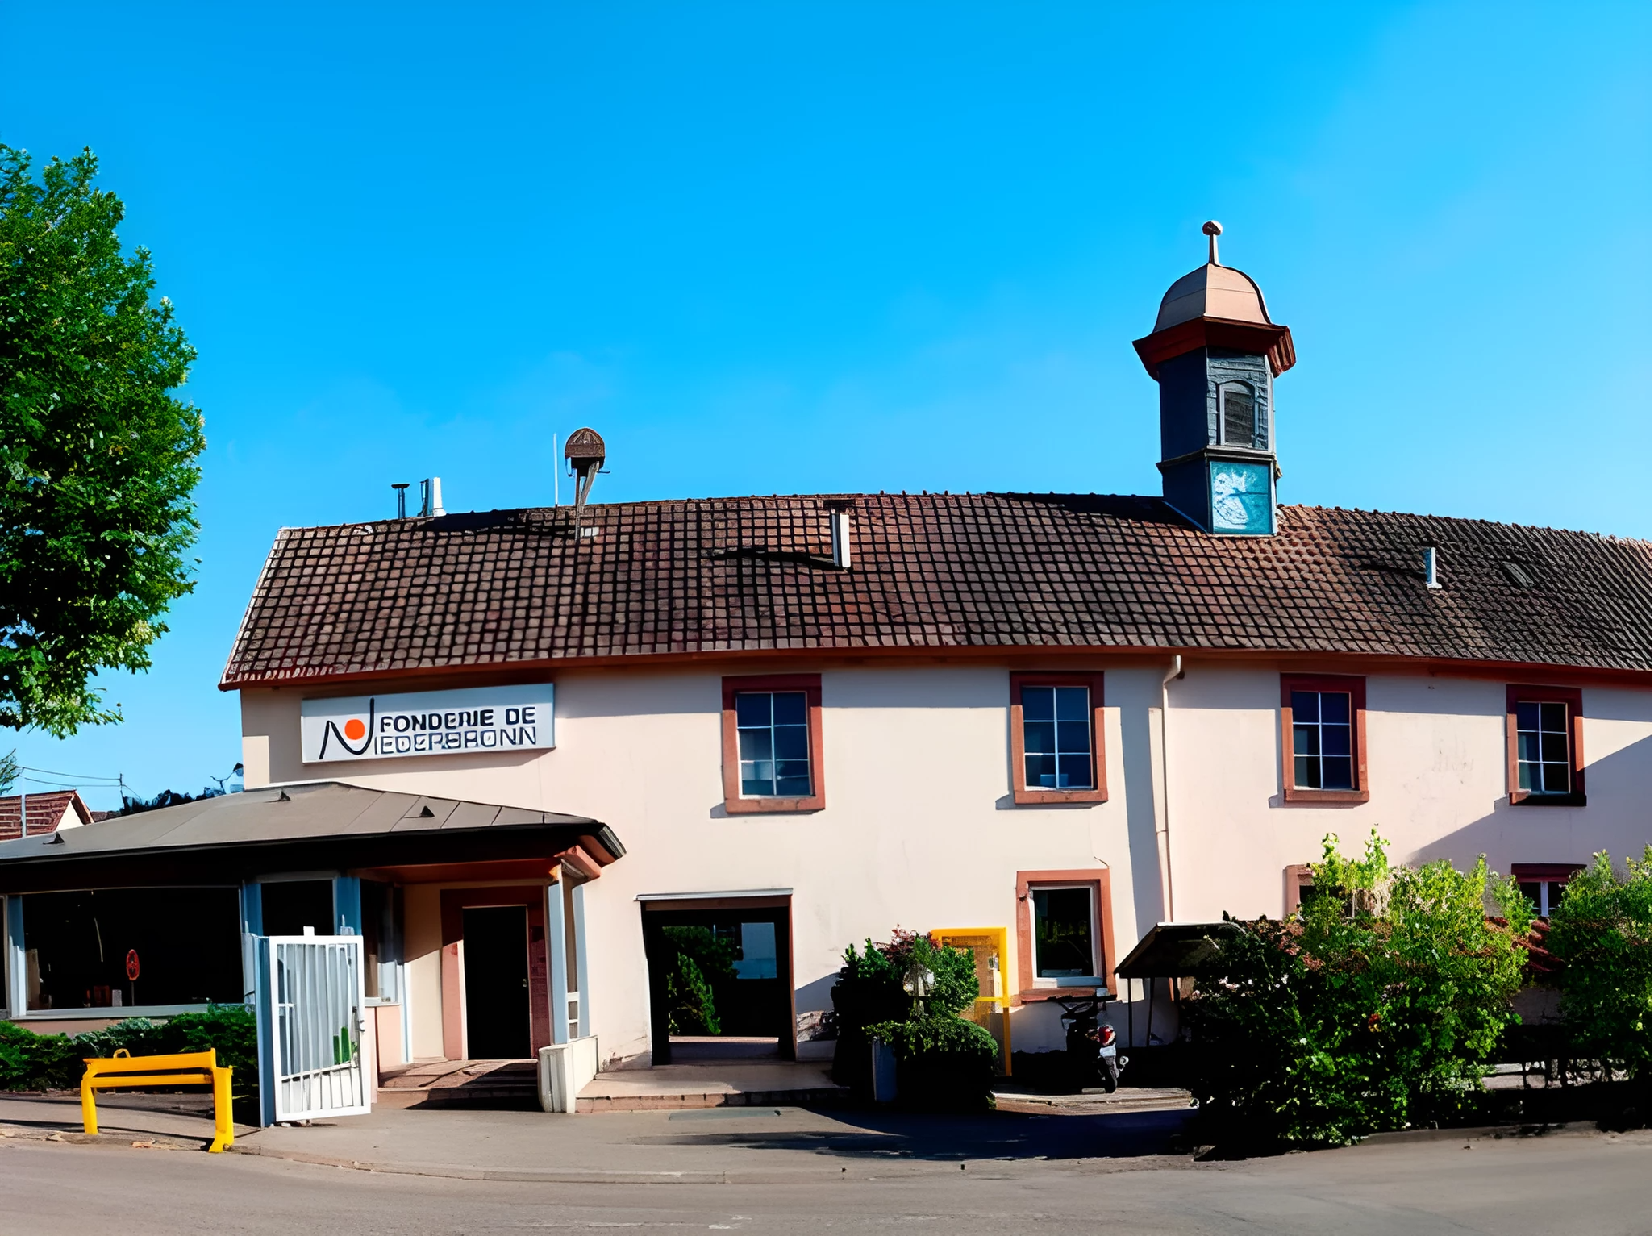
\includegraphics[scale=0.27]{Images/Presentation/Fonderie_vue_de_bas.pdf}
    \hspace{0.5 cm}
    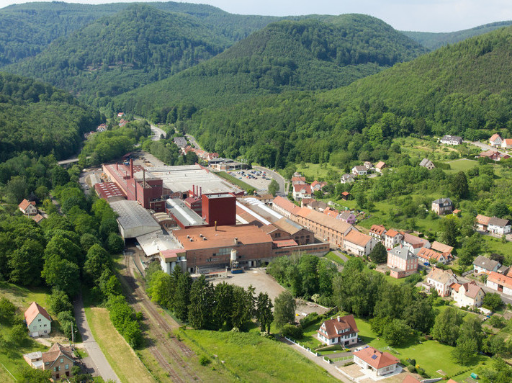
\includegraphics[scale=0.27]{Images/Presentation/Fonderie_vue_de_haut.pdf}
    \caption{Vues extérieure et aérienne de la Fonderie de Niederbronn}
\end{figure}

\newpage

\subsection{Description du processus de production des pièces en fonte}

Voici un schéma décrivant les différents étapes de production d'une pièce en fonte :


% \includepdf[pages=-, scale=1]{Images/Flux de production.pdf}

\begin{figure}[H]
    \centering
    \begin{adjustbox}{width=1.3\textwidth,height=0.8\textheight,center}
        \includegraphics{Images/Presentation/Flux de production.pdf}
    \end{adjustbox}
    \caption{Flux de production des pièces en fonte.}
    \label{fig:flux-production}
\end{figure}


\begin{enumerate}
    \item \textbf{Chargement des matières premières :}
    À cette étape, les matériaux de base nécessaires à la production de la fonte sont 
    préparés. Ce processus implique le tri, le nettoyage et la sélection des matières 
    premières, telles que le fer, le cuivre, les déchets métalliques provenant d'autres 
    industries, et les alliages comme le magnésium et le silicium. Pour obtenir les 
    propriétés mécaniques souhaitées dans la fonte, il est crucial de choisir les 
    matériaux en fonction de leur composition chimique, car certains éléments chimique 
    peuvent nuire à la qualité du produit final. 
    Voici une illustration des matières premières utilisées au sein de la fonderie :

    % ----------------- Mettre image des matières premières

    \begin{figure}[H]
        \centering
        \vfill
        \hspace{0.8 cm}
        \includegraphics[scale=0.7]{Images/Presentation/Fontes d'affinages.pdf}
        \hspace{0.5 cm}
        \includegraphics[scale=0.7]{Images/Presentation/Fontes d'affinages.pdf}
        \caption{Les retours et les Frite Haut Silicium}
    \end{figure}

    \begin{figure}[H]
        \centering
        \vfill
        \hspace{0.8 cm}
        \includegraphics[scale=0.7]{Images/Presentation/Fontes d'affinages.pdf}
        \hspace{0.5 cm}
        \includegraphics[scale=0.7]{Images/Presentation/Fontes d'affinages.pdf}
        \caption{Les retours et les Frite Haut Silicium}
    \end{figure}


    \item \textbf{Fusion :} Une fois les métaux sélectionnée, le métal est fondu dans 
    un four à induction atteignant des températures suffisamment élevées pour le 
    transformer en liquide.



    \item \textbf{Modélage :} 

    Le modélage est l'une des premières étapes de la production en fonderie. Il s'agit 
    de préparer le modèle et le moule nécessaires à la coulée. La pièce finale est 
    d'abord conçue numériquement à l'aide de logiciels de CAO. Une fois la conception 
    terminée, le modèle physique est fabriqué en métal. Le moule est généralement réalisé à partir de sable (mélangé avec de l'argile et 
    de l'eau) compacté autour du modèle. Le sable doit être suffisamment résistant pour supporter le 
    poids du métal fondu sans se désagréger. Une fois le sable compacté, le modèle est retiré, et les parties du moule sont 
    assemblées. Des conduits de coulée sont ajoutés pour permettre au métal fondu de 
    remplir la cavité du moule.

    % ----------------- Mettre image de modèle physique ?!


    \item \textbf{Noyautage :} 
    Le noyautage est une étape essentielle pour créer des formes internes ou des 
    cavités dans la pièce coulée. Comme le moule, les noyaux sont souvent fabriqués 
    en sable. Ils sont formés à l'aide de boîtes à noyaux qui donnent aux noyaux la 
    forme nécessaire. Les noyaux permettent de créer des canaux, des alésages, et 
    d'autres détails internes. Une fois fabriqués, les noyaux sont place avec précision
    dans le moule pour s'assurer qu'ils créent les cavités désirées. Ils doivent être 
    solidement fixer pour éviter tout déplacement lors de la coulée.


    \item \textbf{Sphéroïdisation :} 
    Cette etape ne concerne que les fontes GS. 
    La sphéroïdisation est un processus crucial pour améliorer les propriétés mécaniques 
    de la fonte, notamment sa ductilité et sa résistance.
    Le magnésium est ajouté à la fonte liquide pour favoriser la formation de graphite 
    sphéroïdal plutôt que lamellaire. Cela se fait souvent en ajoutant un alliage 
    contenant du magnésium comme le fil fourrée. Les sphéroïdes de graphite augmentent la ductilité et la résistance de la fonte, 
    ce qui la rend plus adaptée à des applications nécessitant une résistance élevée 
    à la traction. Ce traitement modifie la microstructure de la fonte pour améliorer ses performances
    mécaniques et sa durabilité.


    % ----------------- Mettre image Microscopique de la fonte GS

    \item \textbf{Inoculation et Dégrassage :} Dans cette étape, des agents d'inoculation sont 
    ajoutés au métal fondu pour contrôler la structure et les propriétés finales de 
    la fonte GS. Ces agents favorisent la formation de sphéroïdes de graphite de 
    taille et de forme uniformes.

    L'inoculation est réalisée après la sphéroïdisation pour contrôler la structure 
    et les propriétés finales de la fonte. Des agents inoculants, tels que le 
    ferrosilicium, sont ajoutés pour favoriser une précipitation uniforme et fine 
    du graphite.

    % ----------------- Mettre image Innoculation/Degrassange en action ou du produits innoculant
    
    \item \textbf{Moulage ou Coulée :} La fonte est  versé dans 
    le moule à travers les conduits de coulée pour prendre la forme finale de la pièce. Une 
    fois coulé, le métal liquide refroidit et se solidifie à l'intérieur du moule, prenant la 
    forme de la cavité créée par le modèle et les noyaux.



    \item \textbf{Décochage et Grenaillage :} 

    Après la coulée, Une fois le métal solidifié, le moule est démonté pour extraire 
    la pièce coulée. Les moules en sable sont souvent détruits au cours de ce processus,
    tandis que les moules permanents peuvent être réutilisés. Les noyaux en sable sont 
    retirés, souvent à l'aide de vibrations ou de lavage, pour révéler les cavités 
    internes de la pièce. Grenaillage : La pièce est ensuite nettoyée par projection 
    de billes d'acier (ou d'autres matériaux abrasifs) pour enlever la calamine, les 
    restes de sable et améliorer la surface.
    
    \item \textbf{Ebarbage et Usinage :} 
    La pièce obtenue après démoulage n'est pas encore prête pour une utilisation directe. 
    Elle doit subir plusieurs opérations de finition. Les pièces sont ébarbées pour 
    enlever les bavures et les excès de métal laissés par les joints du moule ou les 
    conduits de coulée. Les pièces peuvent être usinées pour atteindre des dimensions 
    précises et une surface lisse.
    

    \item \textbf{Peinture :} La peinture et le revêtement sont appliqués à la pièce 
    pour la protéger de la corrosion et lui donner un aspect esthétique. La surface de 
    la pièce est nettoyée et préparée pour une meilleure adhérence de la peinture.
    Des peintures ou des revêtements spécifiques sont appliqués par pulvérisation, 
    trempage ou brossage.



    \item \textbf{Contrôle qualité et Livraison :} Avant la livraison des pièces finales, un 
    contrôle qualité est effectué pour s'assurer qu'elles répondent aux normes et 
    aux spécifications requises. La composition chimique de la pièce est analysée pour 
    s'assurer qu'elle correspond aux spécifications. Des tests de traction, de dureté, 
    et d'impact peuvent être effectués pour valider les propriétés mécaniques de la 
    pièce.
\end{enumerate}



\subsection{L'objectif du stage }


% Presenter rapidement L'objectif du stage
L’objectif principal de ce stage est d’optimiser l’utilisation des matières 
premières recyclées dans la production de fonte à hautes caractéristiques 
mécaniques. Le projet s’inscrit dans le cadre d’un crédit d’impôt recherche 
et vise à modéliser et automatiser les processus liés au choix et aux 
quantités des différentes matières premières. Voici les missions confiées :

\begin{itemize}
    \item Modéliser le système via des équations.
    \item Contribuer à l’optimisation des coûts de revient en 
    automatisant les processus.
    \item Participer à d’autres sujets d’optimisation en parallèle.
\end{itemize}


\subsection{Le plan du rapport}

% Presenter rapidement le plan du rapport
Le présent rapport couvre les éléments suivants : la présentation de 
la fonderie de Niederbronn, la description du processus 
de production et de l'objectif du stage, 

mandat du stage la méthodologie utilisée durant le stage, et les résultats du stage. En
fin une conclusion boucle ce rapport de stage.



%---- motiver le sujet et objectif stage


%---- détail objectif stage





\section{L'étude statistique}

% Contexte et Objectifs

\subsection{Contexte et Objectifs}

Nous disposons de 2 mesures normatives la résistance mécanique en MPA et l'allongement 
en pourcentage , de la composition chimique de la fonte étudiée obtenus grâce au 
spectromètre et de 5 indicateurs de qualités, qui sont des combinaisons d'éléments 
chimiques.
L'objectif est d'évaluer la pertinance des 5 indicateurs de qualités à la vue 
des 2 mesures normatives et de sélectionner  les meilleurs indicateurs de qualité 
et donner leurs intervalle de prédictions.


\subsection{Les données}

% Source des données

Les données utilisées dans ce projet proviennent de deux sources principales :
une machine de Traction et d'un Spectromètre . 
D'aborb, la résistance mécanique et l'allongement sont mesurées à l'aide d'une 
machine de traction. Ensuite, Les données concernant les éléments chimiques dans 
la fonte sont obtenus à l'aide de spectromètres.


% Format des données

Les données sont au format Données au format Windev extraites dans un fichier Excel.
Le Type de Données est la Base de données. Nous disposons d'une de données et de features .

La Figure ci-dessous ~\ref{fig:donnees_brutes}  illustre l'état initial des données avant tout 
processus de nettoyage ou d'analyse.


% Les données brutes
\begin{figure}[H]
    \centering
    \includegraphics[width=\textwidth]{Images/Statistique/DonnéesBrut1.pdf} \\
    \vspace{10pt}
    \includegraphics[width=\textwidth]{Images/Statistique/DonnéesBrut2.pdf} \\
    \vspace{10pt}
    \includegraphics[width=\textwidth]{Images/Statistique/DonnéesBrut3.pdf}
    \caption{Visualisation des données brutes}
    \label{fig:donnees_brutes}
\end{figure}




    




    
    
% Description des données


\textbf{Les variables quantitatives :}

\begin{itemize}
\item Rm : Résistance mécanique à la traction.
\item Rp0.2 : Limite d'élasticité à 0,2% de déformation.
\item A\% : Allongement à la rupture en pourcentage.
\item Contre-essai A\% : Contre-essai de l'allongement à la rupture en pourcentage.
\item Moyenne allongement : Moyenne de l'allongement à la rupture en pourcentage.
\end{itemize}
    

\textbf{Les indicateurs :}

\begin{itemize}
\item Impureté : Pourcentage d'impureté dans l'échantillon.
\item \% Ferrite : Pourcentage de ferrite dans l'échantillon.
\item ONO, TANIMURA, ... : Un indicateur de qualité en pourcentage.
\item THIELMANN : Un indicateur de qualité en pourcentage.
\end{itemize}
 

\textbf{Les variables qualitatives :}

\begin{itemize}
\item Recette : Nom ou code de la recette associée à l'échantillon.
\item Date : Date à laquelle la coulée a été effectuée.
\item Poche/Four/Barreau : Indication sur la provenance de l'échantillon (poche, four, barreau, etc.).
\item Conforme ? : Indique si l'échantillon est conforme (1) ou non conforme (0) aux critères définis.
\item Pièces : Référence des pièces.
\item Observations : Commentaires ou observations sur l'échantillon.
\item Comment. RQ : Commentaires ou remarques supplémentaires.
\end{itemize}

\textbf{Les éléments chimiques :}

\begin{itemize}
\item C, Si, Mn, P, Cr, Mo, Cu, Sn, Mg, Ce, Ca, Al 
\item Zn, Ti, S, Sn, V, Pb, Al, Bi, B, Te, Sb, As, Ti 
\end{itemize}



% Prétraitement des Données


Avant d'utiliser les données dans l'étude, elles ont été soumises aux prétraitements suivants :

\begin{itemize}
\item Nettoyage des données :
\begin{itemize}
\item Suppression des colonnes : Date, Rp0.2, A\%, Contre-essai A\%, Pièces, Observations, Comment. RQ, PJ, Ca, Ba.
\item Suppression des lignes incomplètes (celles avec des colonnes vides).
\end{itemize}
\item Ajout de l'indicateur Pureté MAYER.
\item Mise en forme des données :
\begin{itemize}
\item Renommage des colonnes.
\item Séparation des données en fonction  du type de recette.
\item Séparation des données en fonction de la conformité de l'échantillon.
\end{itemize}
\end{itemize}
    


% Les données nettoyées
\begin{figure}[H]
    \centering
    \includegraphics[width=\textwidth]{Images/Statistique/DonnéesClean1.pdf} \\
    \vspace{10pt}
    \includegraphics[width=\textwidth]{Images/Statistique/DonnéesClean2.pdf}
    \caption{Visualisation des données nettoyées}
    \label{fig:donnees_nettoyees}
\end{figure}


\subsection{Les indicateurs}



% Les indicateurs


\begin{itemize}
  \item  Evaluer la pertinence des cinq indicateurs de qualité à la vue des deux mesures normatives.
  \item Dans le but d'évaluer l'influence globale des différents éléments sur la matrice ou la forme du graphite, plusieurs formules ont été proposées par divers auteurs.
\end{itemize}

Voici les 5 formules, qui consistent en une somme pondérée des éléments chimiques :


\begin{align*}
    \textcolor{blue}{\text{Pureté MAYER \%}} &= \text{Ti\%} + \text{Pb\%} + \text{Bi\%} + \text{Sb\%} \\
    \textcolor{red}{\text{Ferrite \%}} &= 92.3 - 96.2 (\text{Mn \%}) - 211 (\text{Cu \%}) - 14270 (\text{Pb \%}) - 2815 (\text{Sb \%}) \\
    \textcolor{green}{\text{Pureté ONO \%}} &= \text{Cu \%} + \text{Ti \%} + \text{Ni \%} + \text{Cr \%} + \text{V \%} + \text{Al \%} + \text{As \%}  + \text{Sn \%} + \text{Pb \%} + \text{Sb \%} \\
    &\quad + \text{Bi \%} \\
    \textcolor{purple}{\text{Impureté \%}} &= 4.9 (\text{Cu \%}) + 0.37 (\text{Ni \%}) + 0.37 (\text{Cr \%})  + 7.9 (\text{Mo \%}) + 4.4 (\text{Ti \%}) + 39.0 (\text{Sn \%}) \\ 
    &\quad + 0.44 (\text{Mn \%}) + 5.6 (\text{P \%}) \\
    \textcolor{orange}{\text{Pureté THIELMANN \%}} &= 4.4 (\text{Ti \%}) + 2.0 (\text{As \%}) + 2.3 (\text{Sn \%}) + 5.0 (\text{Sb \%}) + 290 (\text{Pb \%}) + 370 (\text{Bi \%}) \\
    &\quad + 1.6 (\text{Al \%})
\end{align*}


\begin{align*}
    \textcolor{blue}{\text{Pureté MAYER \%}} &= \text{Ti\%} + \text{Pb\%} + \text{Bi\%} + \text{Sb\%} \\
    \textcolor{red}{\text{Ferrite \%}} &= 92.3 - 96.2 (\text{Mn \%}) - 211 (\text{Cu \%}) \\
    &\quad - 14270 (\text{Pb \%}) - 2815 (\text{Sb \%}) \\
    \textcolor{green}{\text{Pureté ONO \%}} &= \text{Cu \%} + \text{Ti \%} + \text{Ni \%} + \text{Cr \%} + \text{V \%} + \text{Al \%} \\
    &\quad + \text{As \%}  + \text{Sn \%} + \text{Pb \%} + \text{Sb \%} + \text{Bi \%} \\
    \textcolor{purple}{\text{Impureté \%}} &= 4.9 (\text{Cu \%}) + 0.37 (\text{Ni \%}) + 0.37 (\text{Cr \%}) \\
    &\quad + 7.9 (\text{Mo \%}) + 4.4 (\text{Ti \%}) + 39.0 (\text{Sn \%}) \\
    &\quad + 0.44 (\text{Mn \%}) + 5.6 (\text{P \%}) \\
    \textcolor{orange}{\text{Pureté THIELMANN \%}} &= 4.4 (\text{Ti \%}) + 2.0 (\text{As \%}) + 2.3 (\text{Sn \%}) \\
    &\quad + 5.0 (\text{Sb \%}) + 290 (\text{Pb \%}) + 370 (\text{Bi \%}) \\
    &\quad + 1.6 (\text{Al \%})
    \end{align*}
    

    



% Voici la méthode utiliser  pour les classsememt sur la plus grande valeur de (|Rm| + |Allongement|)/2

% La corrélation de Pearson


Pour évaluer nos indicateurs, nous utilisons la corrélation de Pearson afin de quantifier la relation linéaire entre ces derniers et les mesures d'allongement et de résistance mécanique.

\vspace{10pt}
Les étapes de l'évaluation sont les suivantes :
\vspace{5pt}

\begin{enumerate}
\item Calcul des coefficients de corrélation.
\item Classement des indicateurs en fonction de leur corrélation avec l'allongement et la résistance mécanique.
\item Conservation des indicateurs présentant la dépendance linéaire la plus significative avec les deux mesures normatives.
\end{enumerate}



% Évaluation des indicateurs 

\textbf{Corrélation entre les indicateurs et les mesures normatives} 
\begin{figure}[H]
    \includegraphics[width=\textwidth]{Images/Statistique/Matrice_corrélation_qualite_indicateur.pdf} 
\end{figure}


\textbf{ Classement des indicateurs :}
\begin{itemize}
    \item Impureté [\%] : 0.673506
    \item Pureté ONO [\%] : 0.583101
    \item Pureté THIELMANN [\%] : 0.353988
    \item Pureté MAYER [\%] : 0.346637
    \item Ferrite [\%] : 0.327601
\end{itemize}


La matrice de corrélations fournit des informations précieuses sur les relations entre différentes variables de notre jeu de données. Ces corrélations peuvent non seulement aider à prédire une variable en fonction d'une autre, mais aussi à comprendre les interactions et les influences entre les variables. Voici les principales observations :

Une forte corrélation positive (0.65) a été observée entre “Rm [MPa]” et “Moyenne alignement [\%]”. Cela indique que lorsque la résistance à la traction (Rm) augmente, la moyenne d'alignement a également tendance à augmenter.
De même, une forte corrélation positive (0.62) entre “Rm [MPa]” et “Purete ONO [\%]” montre que l'augmentation de la pureté ONO est généralement associée à une résistance à la traction plus élevée.

Une très forte corrélation positive (0.86) a été identifiée entre “Moyenne alignement [\%]” et “Ferrite [\%]”. Cette relation suggère que les niveaux de ferrite augmentent parallèlement à l'amélioration de l'alignement moyen, ce qui pourrait indiquer des mécanismes sous-jacents communs influençant ces deux variables.
Une corrélation négative (-0.41) entre “Rm [MPa]” et “Ferrite [\%]” indique que des niveaux plus élevés de ferrite sont associés à une diminution de la résistance à la traction. Cela pourrait impliquer que la présence de ferrite a un effet affaiblissant sur le matériau.

Une corrélation négative notable (-0.52) entre “Rm [MPa]” et “Purete THIELMANN [\%]” suggère qu'une pureté THIELMANN plus élevée est liée à une réduction de la résistance à la traction.




\subsection{Les éléments chimiques}



%  Les éléments chimiques

Examinons de près les éléments chimiques qui composent l'impureté, la pureté ONO et le taux de ferrite.

Selon la littérature, on classe les éléments chimiques en plusieurs catégories :

\begin{itemize}
    \item \textbf{Les éléments d'alliage :}  C, Si, Mn, P, Cr, Mo, Cu, Sn 
    \item \textbf{Les éléments de traitement :} Mg, Ce, Ca, Al
    \item \textbf{Les éléments polluants :}  Zn, Ti, S, Sn, V 
    \item \textbf{Les éléments poisons :}  Pb, Al, Bi, B, Te, Sb, As, Ti
\end{itemize}
\vspace{5pt}
Dans la formule de la pureté ONO, on retrouve les 4 types d'éléments.
Quant à l'impureté, elle quantifie des éléments poisons, des éléments polluants et des éléments d'alliage.



% Impureté

\textbf{Corrélation entre l'impureté et les éléments chimiques} 

\begin{figure}[H]
    \includegraphics[width=\textwidth]{Images/Statistique/Matrice_corrélation_Impurete_Elements.pdf} 
\end{figure}

\textbf{Classement des éléments chimiques :}
\begin{itemize}
    \item Sn (Étain) [\%] : 0.902219
    \item Cu (Cuivre) [\%] : 0.753903
    \item Cr (Chrome) [\%] : 0.522274
\end{itemize}


Une forte corrélation positive (0.88) est observée entre le Chrome (Cr) et le Molybdène (Mo). 
Les impuretés montrent une corrélation modérément positive avec le Nickel (Ni) et le Titane (Ti), toutes deux à 0.36. Cela indique que les niveaux de ces impuretés ont tendance à augmenter modérément lorsque la concentration de Ni ou de Ti augmente.
Les corrélations entre les impuretés et des éléments tels que le Cuivre (Cu), le Manganèse (Mn), et le Phosphore (P) sont faibles, avec des valeurs proches de 0. Cela suggère qu'il n'y a pas de relation significative entre ces éléments et les impuretés dans le contexte étudié.

% Purete ONO


\textbf{Corrélation entre la purete ONO et les éléments chimiques}
\begin{figure}[H]
    \includegraphics[width=\textwidth]{Images/Statistique/Matrice_corrélation_ONO_Elements.pdf} 
\end{figure}

\textbf{Classement des éléments chimiques : }
\begin{itemize}
    \item Cu (Cuivre) [\%] : 0.934031
    \item Cr (Chrome) [\%] : 0.707962
    \item Sn (Étain) [\%] : 0.606912
    \item Ni (Nickel) [\%] : 0.590721
    \item V (Vanadium) [\%] : 0.527861
\end{itemize}

La pureté ONO [%] a une forte corrélation positive avec Cu [%] (0.93) et Ti [%] (0.92).
Il y a des corrélations positives modérées avec Ni [%] (0.59) et Cr [%] (0.53)
Les éléments comme Sb [%], Bi [%], et Al [%] montrent des corrélations faibles ou négligeables avec la pureté ONO, suggérant qu’ils n’ont pas un impact significatif sur celle-ci.




% Ferrite

% \textbf{Corrélation entre la Ferrite et les éléments chimiques} 
% \begin{figure}[H]
%     \includegraphics[width=\textwidth]{Images/Statistique/Matrice_corrélation_Ferrite_Elements.pdf} 
% \end{figure}

% \textbf{Classement des éléments chimiques : }
% \begin{itemize}
%     \item Cu (Cuivre) [\%] : -0.66
%     \item Sb (Antimoine) [\%] : -0.64
%     \item Mn (Manganèse) [\%] : -0.54
% \end{itemize}


% Ferrite et Purete ONO 
\begin{figure}[H]
    \centering
    \begin{adjustbox}{width=1.3\textwidth,center}
        \includegraphics[scale=1]{Images/Statistique/Matrice_corrélation_ONO_Elements.pdf}
        \includegraphics[scale=1]{Images/Statistique/Matrice_corrélation_Ferrite_Elements.pdf}
    \end{adjustbox}
    \caption{Matrices de corrélation La Purete ONO et la ferrite avec leurs éléments chimique.}
    \label{fig:correlations Ferrite_ONO}
\end{figure}

La pureté ONO [%] a une forte corrélation positive avec Cu [%] (0.93) et Ti [%] (0.92).
Il y a des corrélations positives modérées avec Ni [%] (0.59) et Cr [%] (0.53)
Les éléments comme Sb [%], Bi [%], et Al [%] montrent des corrélations faibles ou négligeables avec la pureté ONO, suggérant qu’ils n’ont pas un impact significatif sur celle-ci.


La Ferrite [%] a une forte corrélation négative avec Sb [%] (-0.64) et Cu [%] (-0.66), 
Il y a une corrélation négative modérée avec Mn [%] (-0.54)
Les autres éléments montrent des corrélations faibles ou négligeables avec la Ferrite, suggérant qu’ils n’ont pas un impact significatif sur celle-ci.





% Pureté THIELMANN

% \textbf{Corrélation entre la Pureté THIELMANN et les éléments chimiques} 
% \begin{figure}[H]
%     \includegraphics[width=\textwidth]{Images/Statistique/Matrice_corrélation_THIELMANN_Elements.pdf} 
% \end{figure}



% Pureté MAYER

% \textbf{Corrélation entre la Pureté MAYER et les éléments chimiques} 
% \begin{figure}[H]
%     \includegraphics[width=\textwidth]{Images/Statistique/Matrice_corrélation_MAYER_Elements.pdf} 
% \end{figure}

% \textbf{Classement des éléments chimiques : }
% \begin{itemize}
%     \item 
%     \item 
%     \item 
% \end{itemize}




% Pureté THIELMANN et Pureté MAYER 
\begin{figure}[H]
    \centering
    \begin{adjustbox}{width=1.3\textwidth,center}
        \includegraphics[scale=1]{Images/Statistique/Matrice_corrélation_THIELMANN_Elements.pdf}
        \includegraphics[scale=1]{Images/Statistique/Matrice_corrélation_MAYER_Elements.pdf}
    \end{adjustbox}
    \caption{Matrices de corrélation des éléments de la Pureté THIELMANN et de la Pureté MAYER.}
    \label{fig:correlations}
\end{figure}


La pureté THIELMANN [%] a une forte corrélation positive avec Bi [%] (0.93), ce qui signifie que des niveaux élevés de pureté THIELMANN sont associés à des niveaux plus élevés de bismuth.
Il y a une corrélation positive modérée avec Sb [%] (0.43)
Les éléments comme Ti [%], As [%], et Al [%] montrent des corrélations faibles ou négligeables avec la pureté THIELMANN, suggérant qu’ils n’ont pas un impact significatif sur celle-ci.

Sur Mayer : Il y a une forte corrélation positive entre Ti [%] et Bi [%] (0.69)
Sur Mayer : Sb [%] montre une corrélation négative modérée avec Ti [%] (-0.62)




% Conclusion de la partie corrélation

% Rajoute un texte à ce niveau

\textbf{Les indicateurs les plus pertinants}
\begin{itemize}
\item Impureté : 0.673506
\item Pureté ONO : 0.583101
\end{itemize}

\textbf{Les éléments chimiques conservés}
\begin{itemize}
\item Sn (Étain) 
\item Cu (Cuivre)
\item Cr (Chrome) 
\item V (Vanadium)
\end{itemize}






\subsection{Les valeurs extrêmes}

% Gestions des valeurs extrèmes


Pour améliorer la performance de la régression linéaire, nous procédons à la suppression des valeurs extrêmes basées sur les mesures d'impureté, de pureté ONO et de taux de ferrite. Voici la procédure suivie :

\begin{itemize}
    \item \textbf{Objectif} : Réduire la variabilité des données pour une meilleure performance de la régression linéaire.
    \item \textbf{Critère de suppression } : Une valeur est considérée comme extrême si elle se situe en dehors de l'intervalle défini par $[\bar{x} - 1.5(Q_3 - Q_1), \bar{x} + 1.5(Q_3 - Q_1)]$, où $Q_1$ et $Q_3$, le premier et le troisième quartile de la distribution des données, et $\bar{x}$ la moyenne des données.
    \item Cette suppression est réalisée de manière itérative jusqu'à ce qu'il n'y ait plus de valeurs extrêmes dans l'ensemble de données.
\end{itemize}




% Les valeurs extrèmes de l'impurté

\begin{figure}[H]
    \includegraphics[width=\textwidth]{Images/Statistique/Impureté_avec_extreme.pdf}
    \includegraphics[width=\textwidth]{Images/Statistique/Impureté_sans_extreme.pdf}
    %  \textwidth
\end{figure}


% Les valeurs extrèmes de l'impurté
\begin{figure}[H]
    \centering
    \begin{adjustbox}{width=1.3\textwidth,center}
        \includegraphics[scale=1]{Images/Statistique/Impureté_avec_extreme.pdf}
        \includegraphics[scale=1]{Images/Statistique/Impureté_sans_extreme.pdf}
    \end{adjustbox}
    \caption{Les valeurs extrèmes de l'impurté.}
    \label{fig:Extrem}
\end{figure}


% Les valeurs extrèmes de l'impurté
\begin{figure}[H]
    \centering
    \begin{adjustbox}{width=1.3\textwidth,center}
        \includegraphics[scale=1]{Images/Statistique/Impureté_sans_extreme 2.pdf}
        \includegraphics[scale=1]{Images/Statistique/Impureté_sans_extreme 2.pdf}
    \end{adjustbox}
    \caption{Les valeurs extrèmes de l'impurté.}
    \label{fig:Extreme}
\end{figure}



% Les valeurs extrèmes de l'impurté
\begin{figure}[H]
    \centering
    \begin{adjustbox}{width=1.3\textwidth,center}
        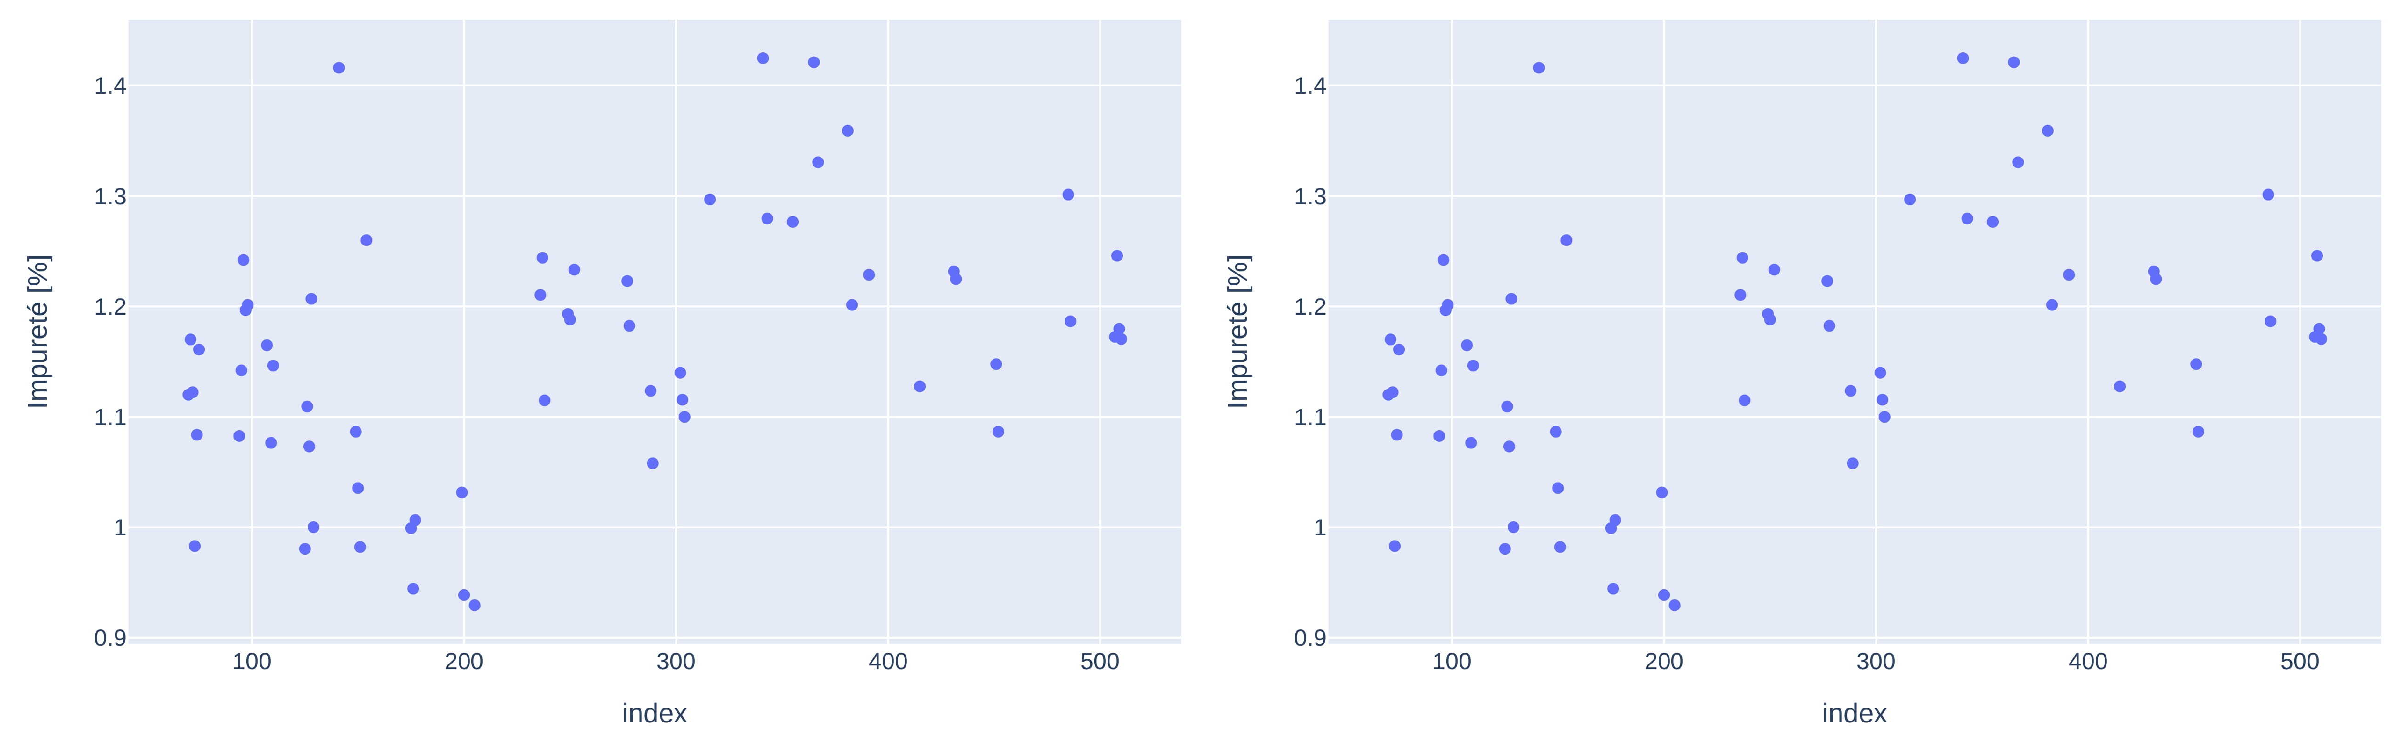
\includegraphics[scale=1]{Images/Statistique/Essais.pdf}
    \end{adjustbox}
\end{figure}

\subsection{La régression linéaire }

% La régression linéaire: Analyse des Données

Effectuons une régression linéaire et calculons les intervalles de  prédictions 
suivant les éléments chimiques et les indicateurs les plus pertinants.


\begin{figure}[H]
    \centering
    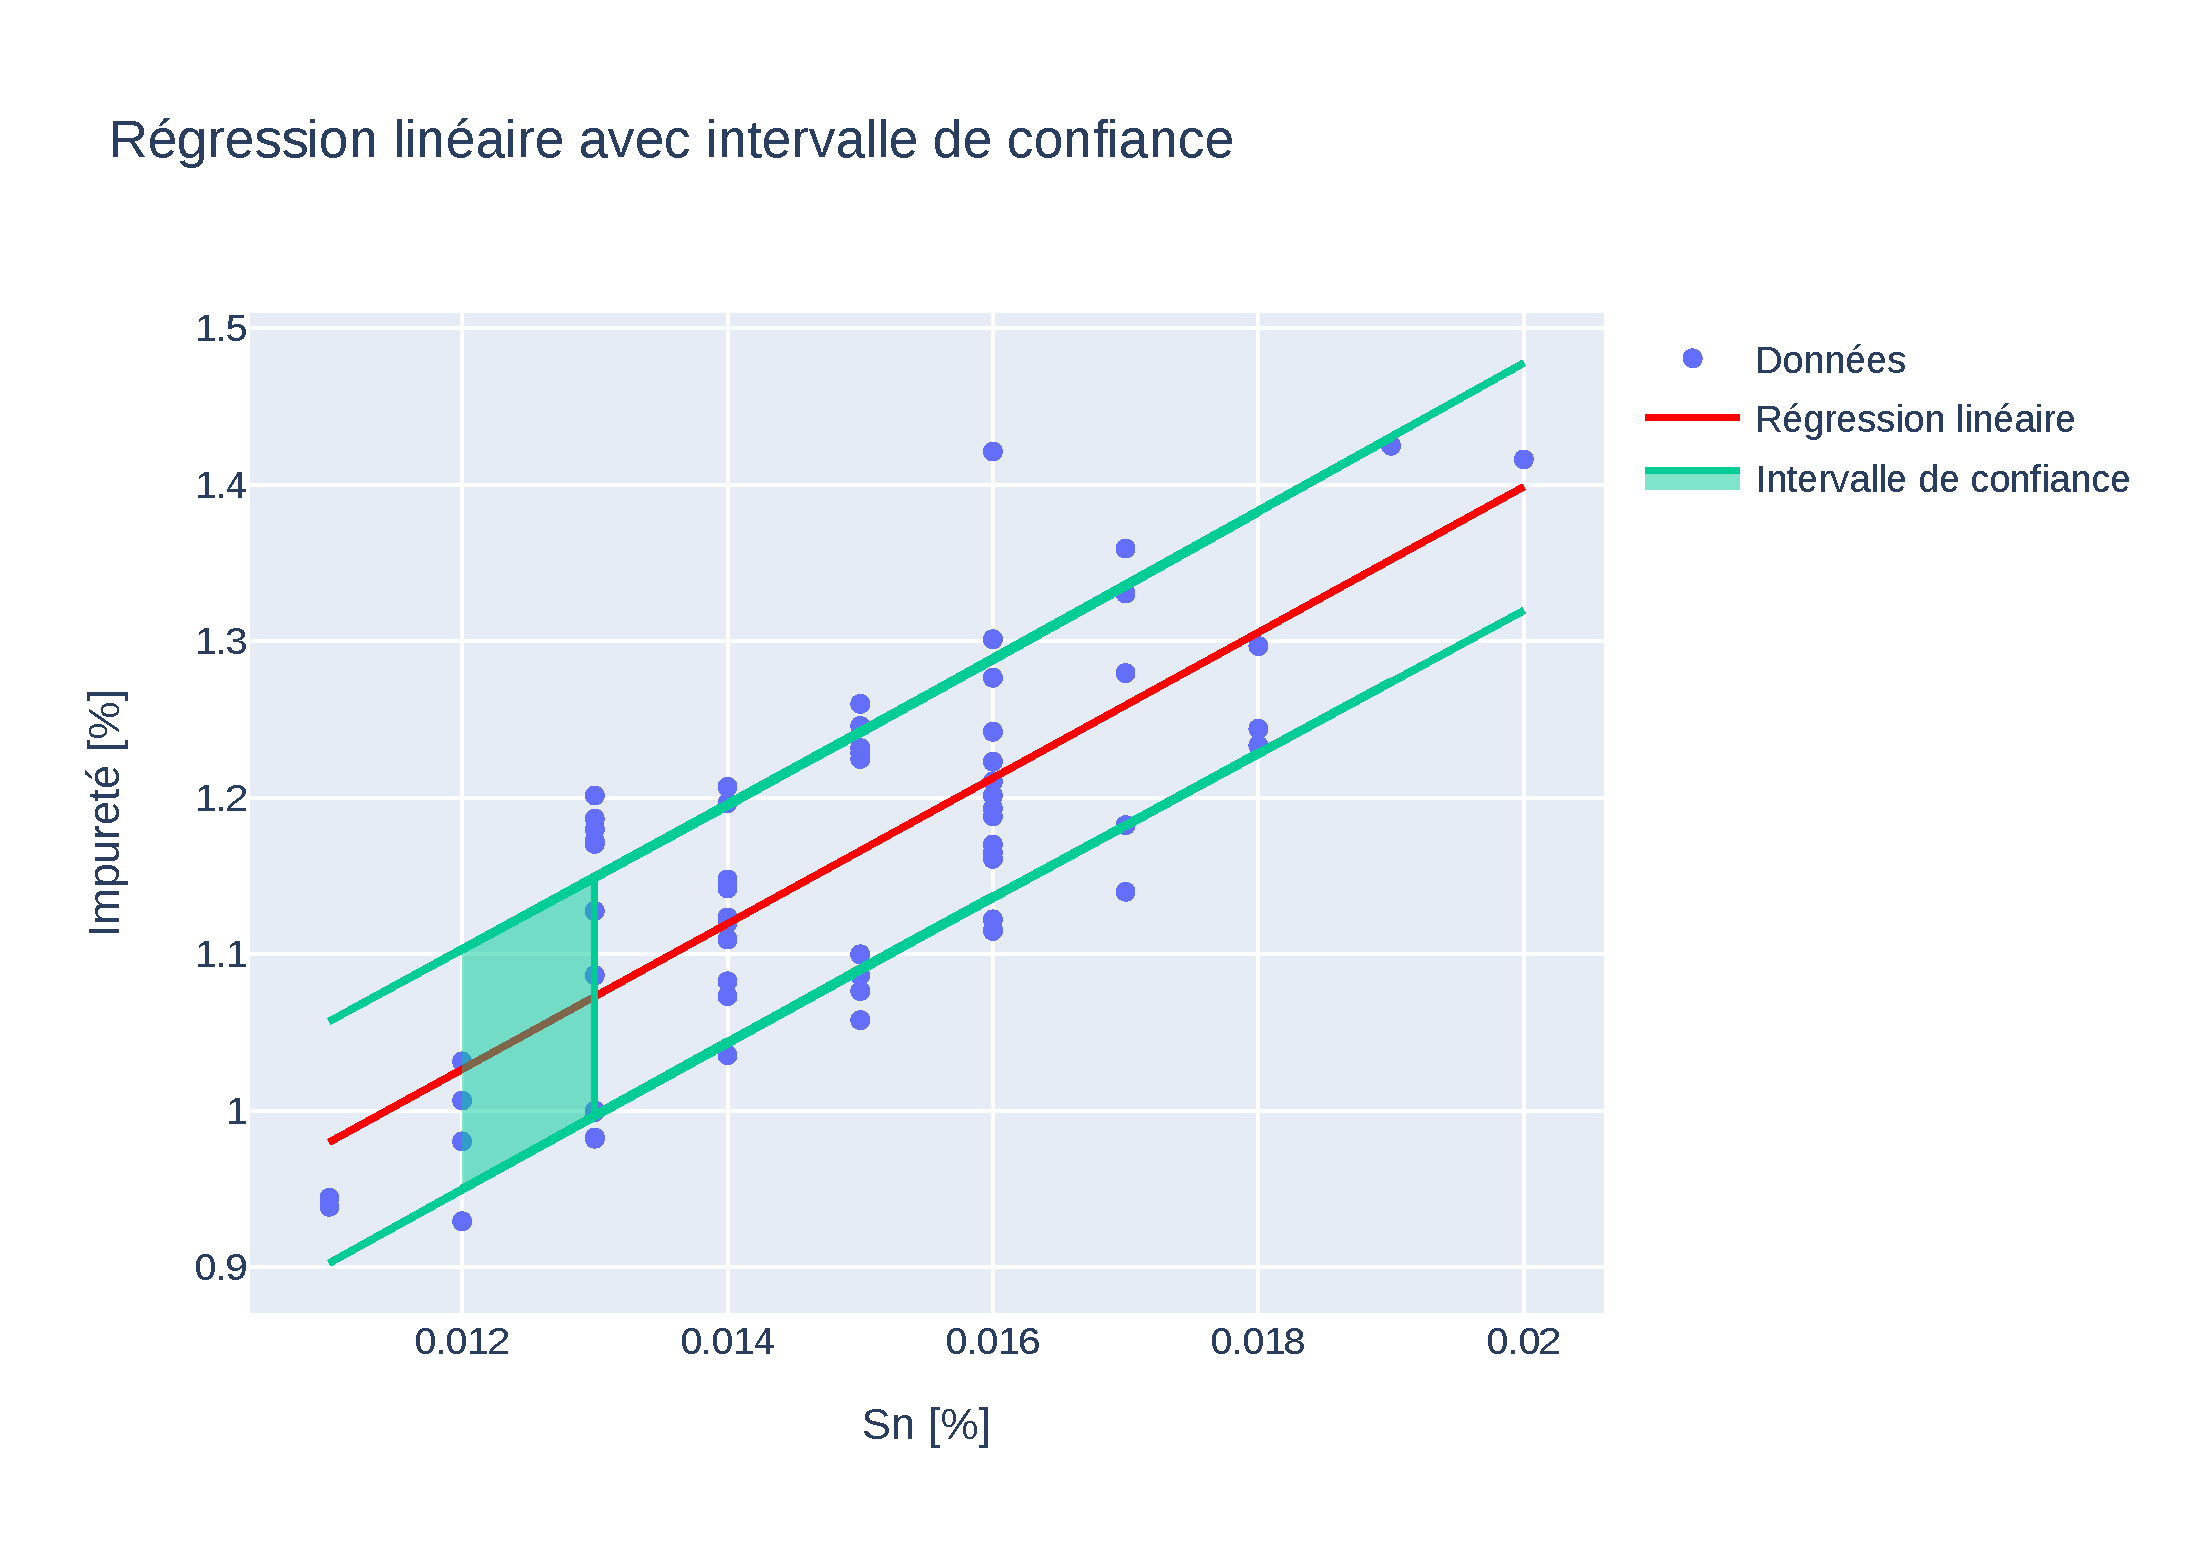
\includegraphics[width=0.9\textwidth]{Images/Statistique/Regression_Impurete_Sn.pdf} % Réduction à 90% de la largeur de texte
    \vspace{10pt} % Espace vertical entre les images
    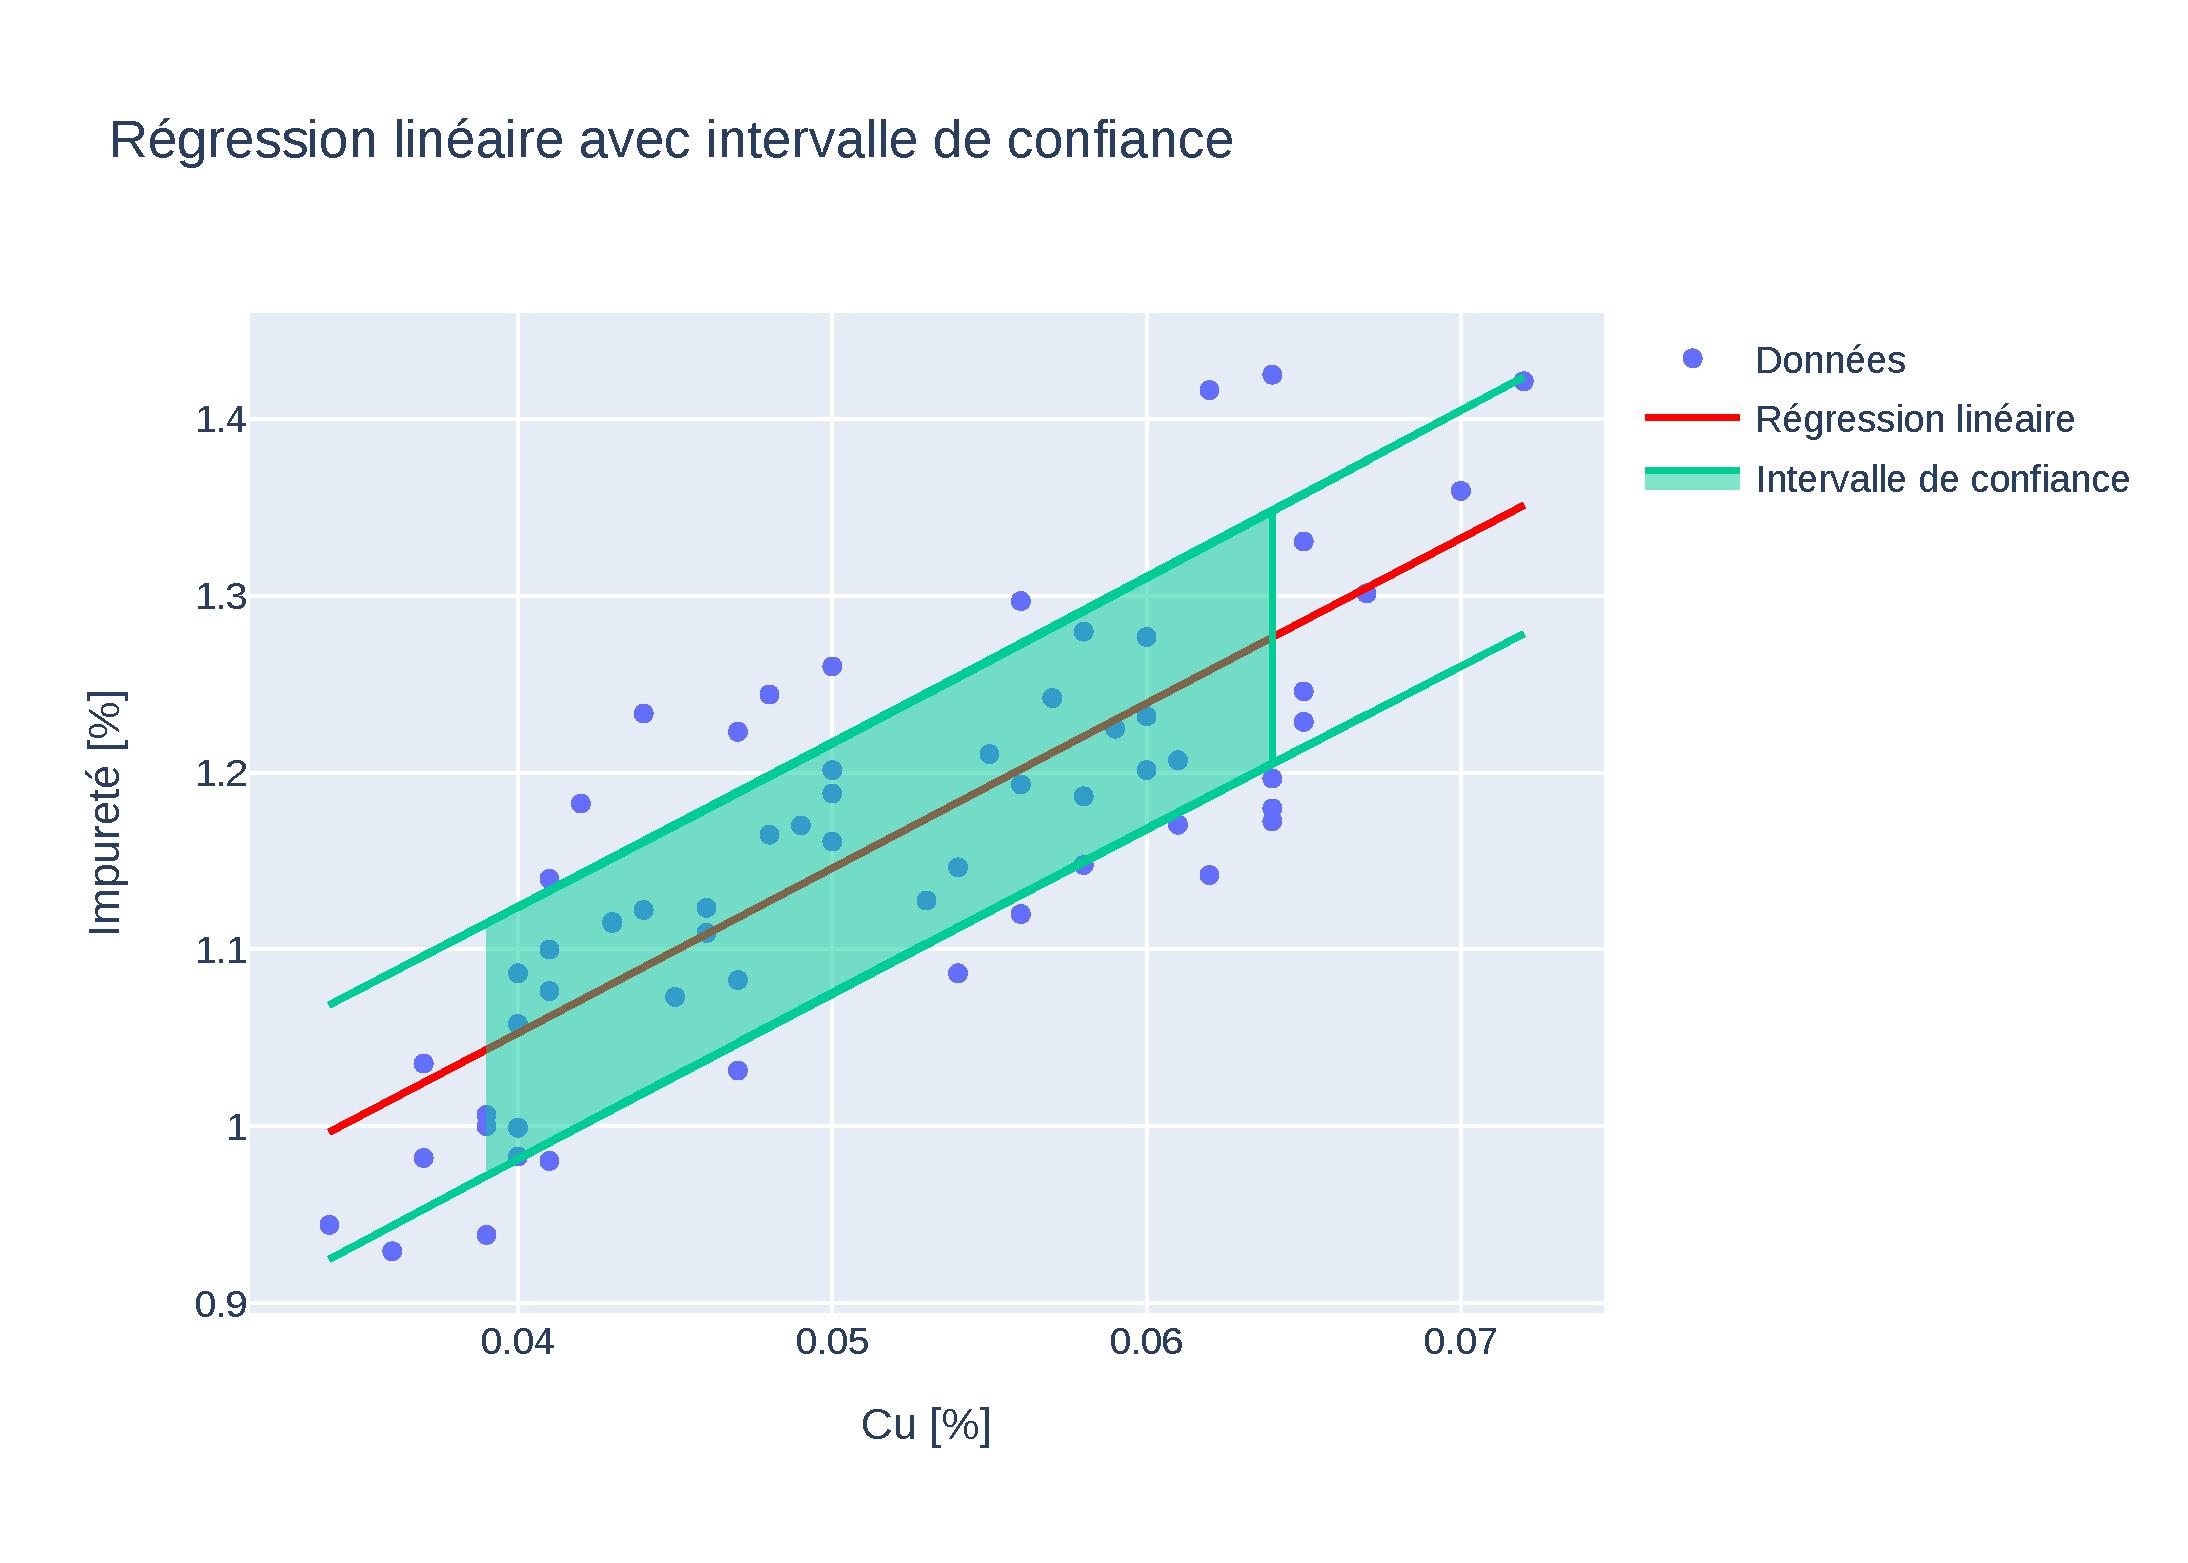
\includegraphics[width=0.9\textwidth]{Images/Statistique/Regression_Impurete_Cu.pdf}
\end{figure}


\begin{figure}[H]
    \centering
    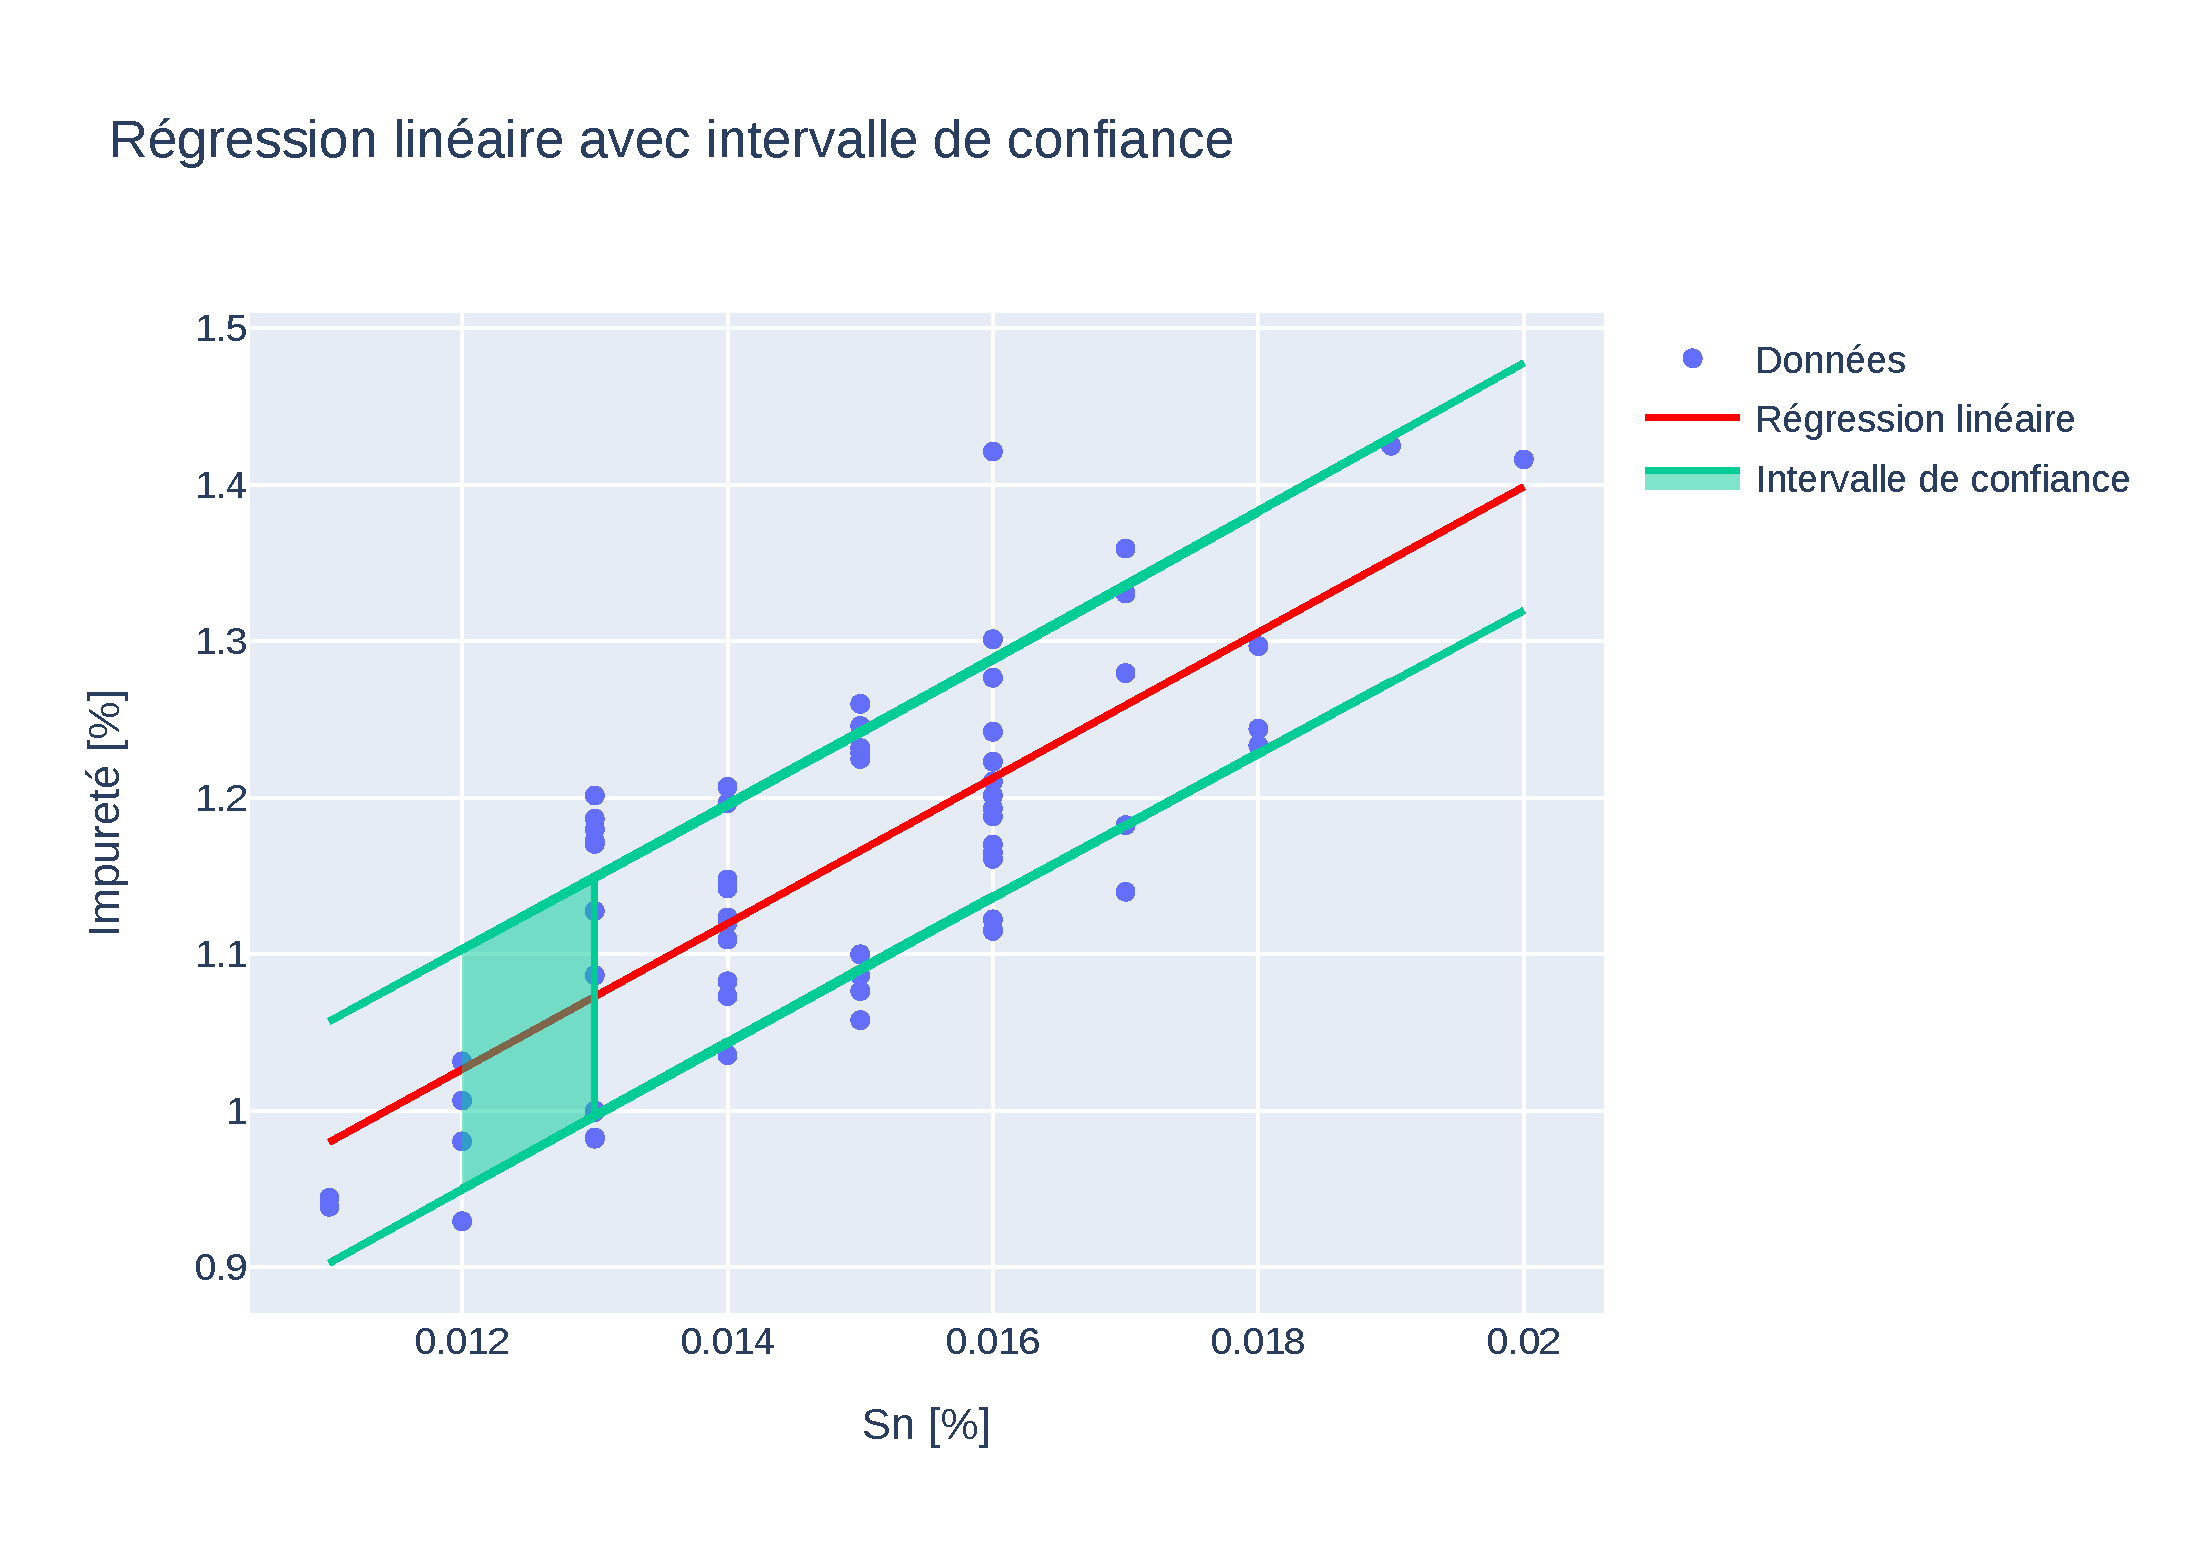
\includegraphics[width=0.45\textwidth]{Images/Statistique/Regression_Impurete_Sn.pdf} 
    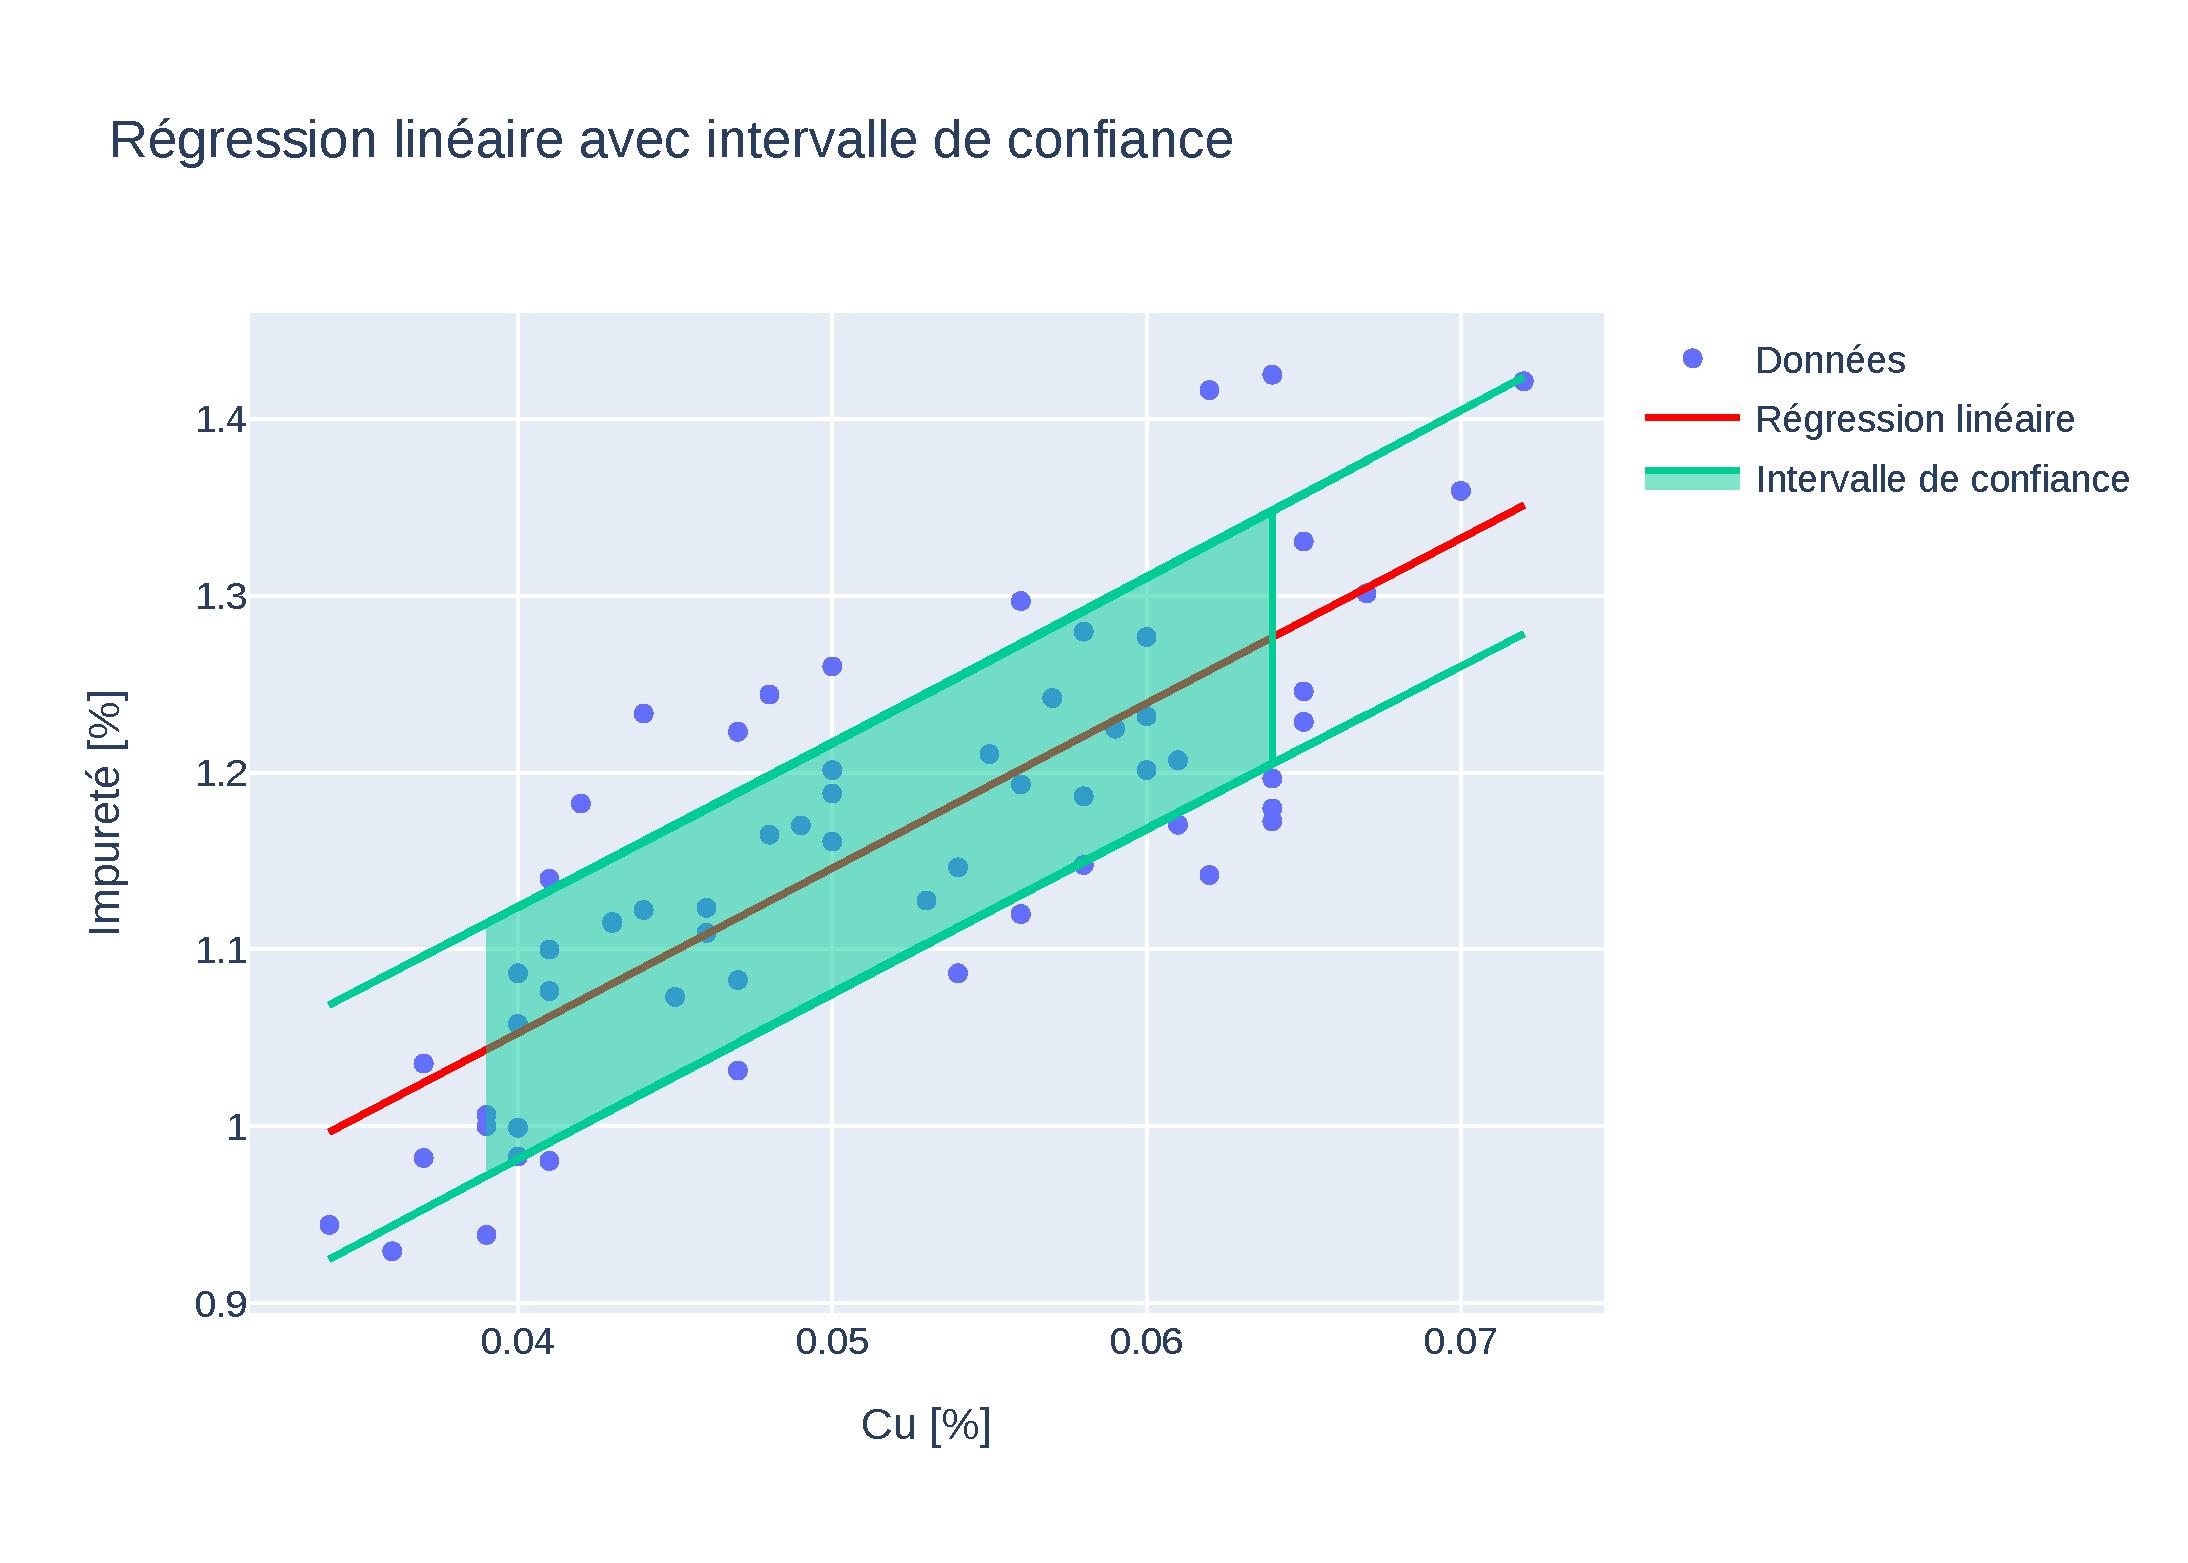
\includegraphics[width=0.47\textwidth]{Images/Statistique/Regression_Impurete_Cu.pdf}
    \caption{Régressions des impuretés pour l'étain (Sn) et le cuivre (Cu).}
    \label{fig:regression-impurete}
\end{figure}


\medskip % Mettre un espace

La formule des intervalles de prédiction est donnée par :
$$
IP (y_{pred}) = [y_{pred} - n \cdot predict\_se, y_{pred} + n \cdot predict\_se]
$$
Où :
\begin{itemize}
    \item $y_{pred}$ est la valeur prédite.
    \item predict\_se est  l'écart-type de prédiction.
    \item  n  est un entier naturel.
\end{itemize}





% Impureté

\textbf{L'impurété en fonction de l'étain (Sn)} 
\begin{figure}[H]
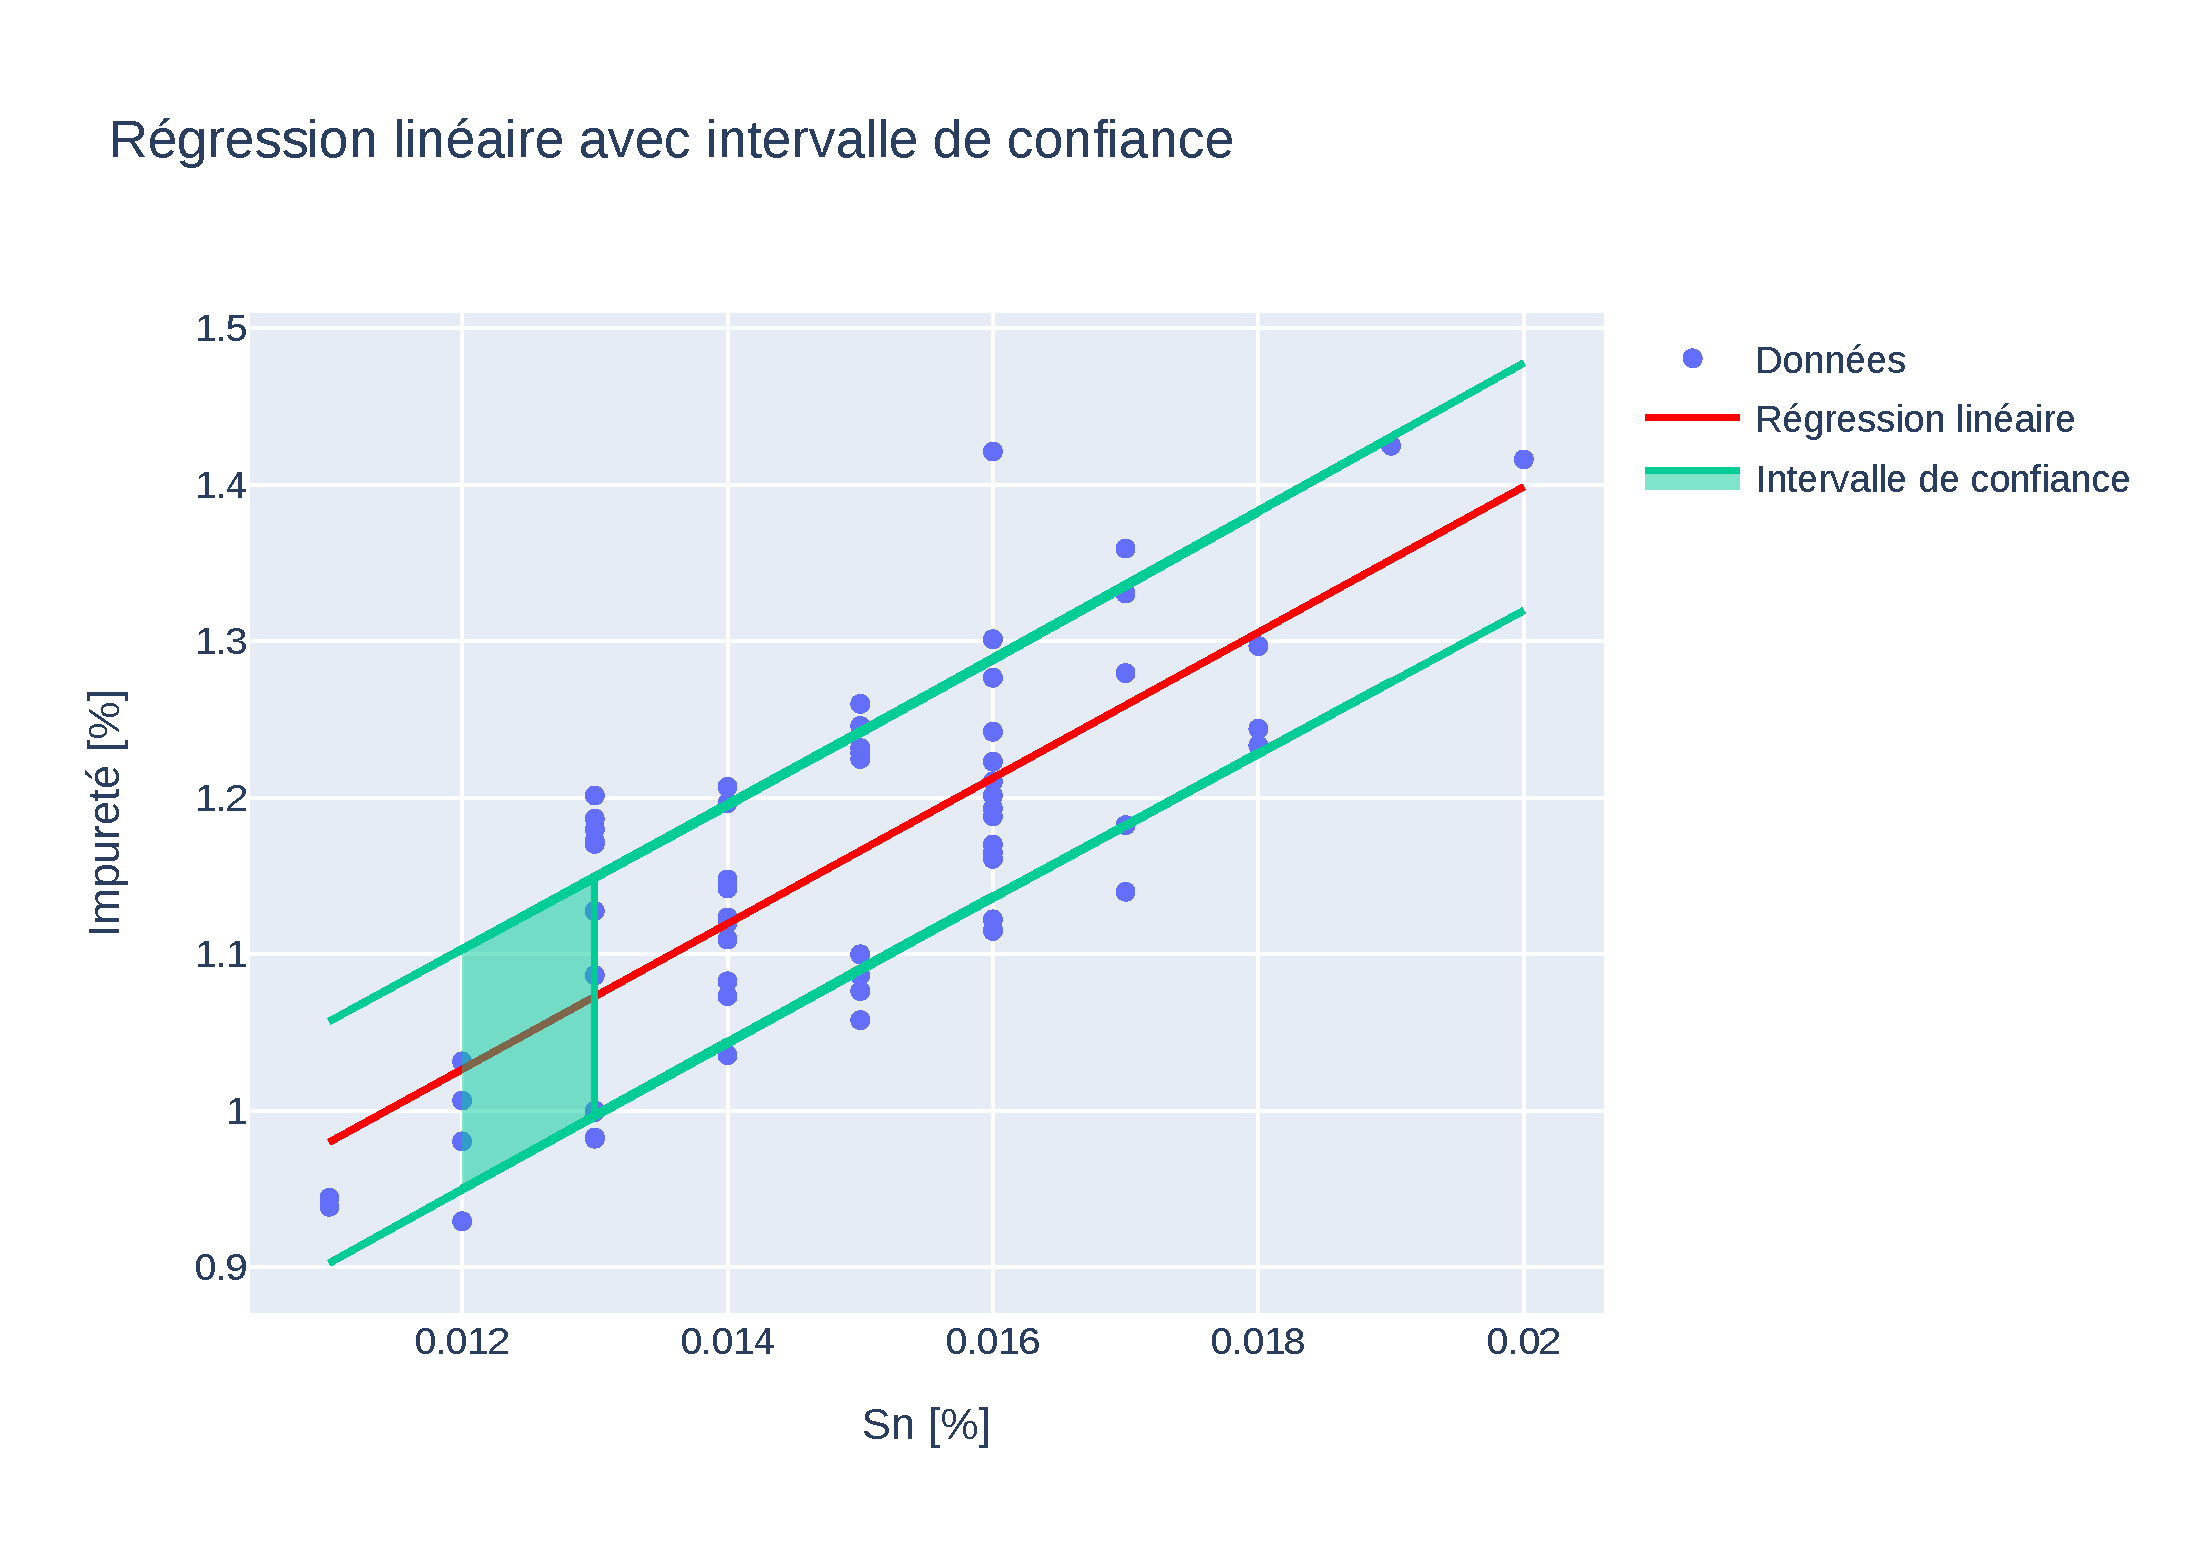
\includegraphics[width=\textwidth]{Images/Statistique/Regression_Impurete_Sn.pdf} 
\end{figure}





\begin{figure}[H]
\textbf{L'impurété en fonction du cuivre (Cu)} 
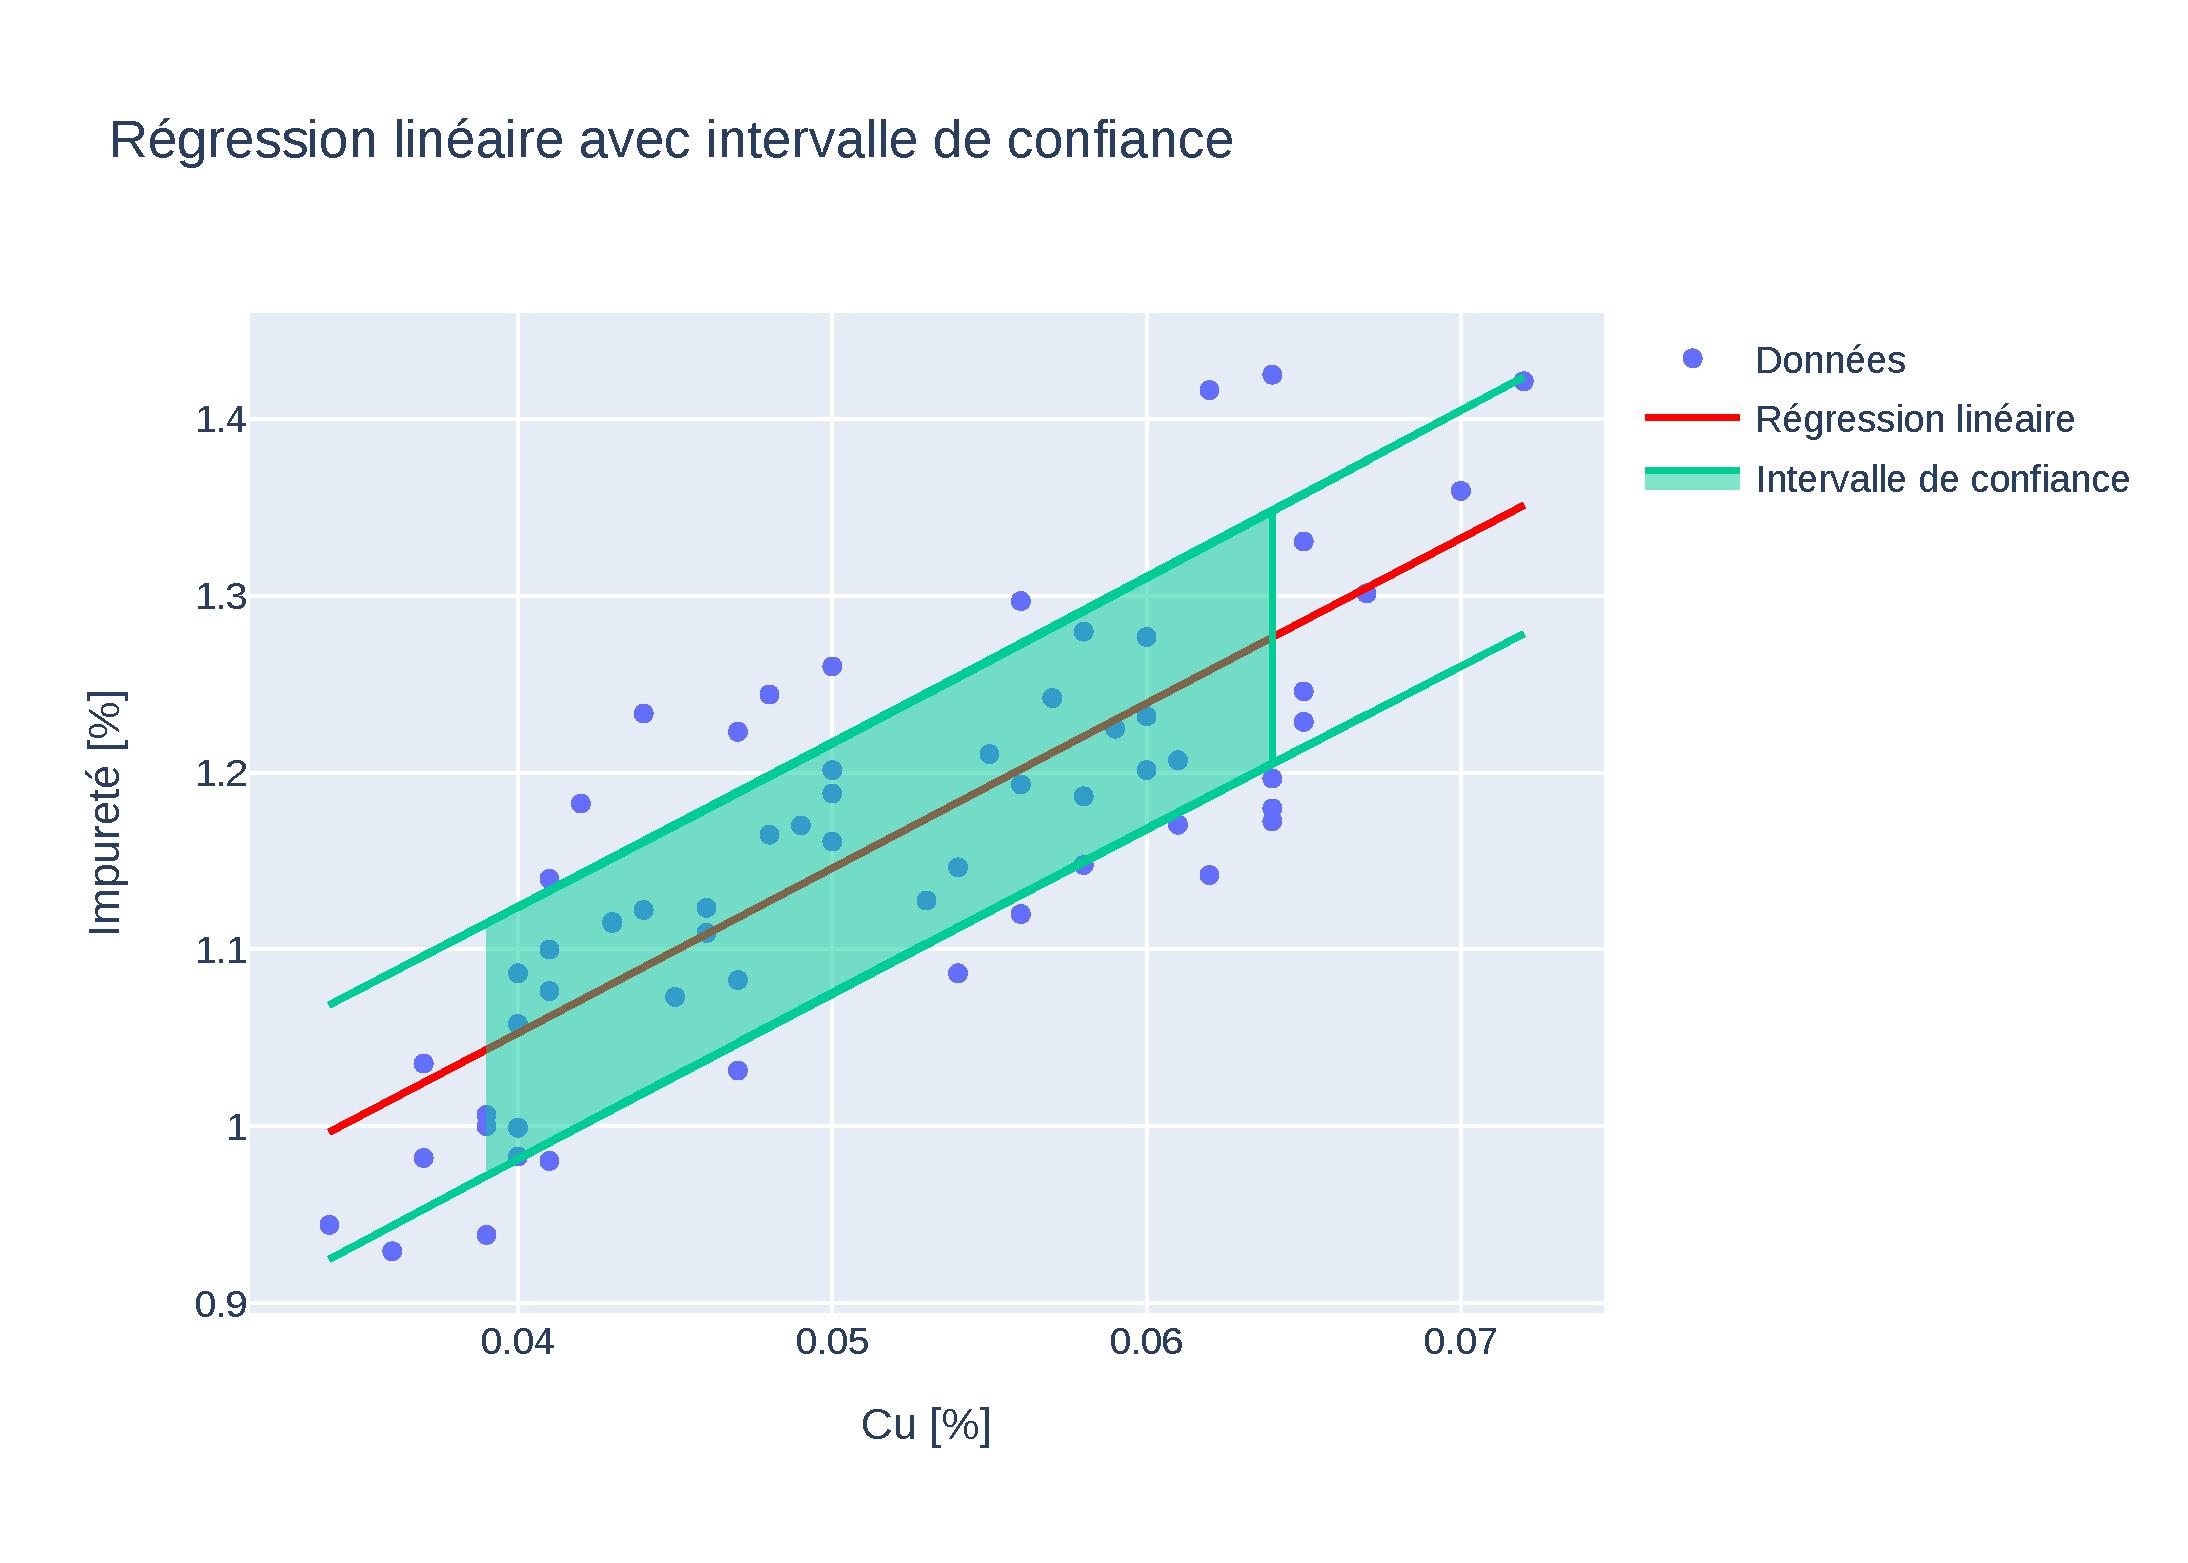
\includegraphics[width=\textwidth]{Images/Statistique/Regression_Impurete_Cu.pdf} 
\end{figure}



% Purete ONO

\textbf{La pureté Ono en fonction du cuivre (Cu)} 
\begin{figure}[H]
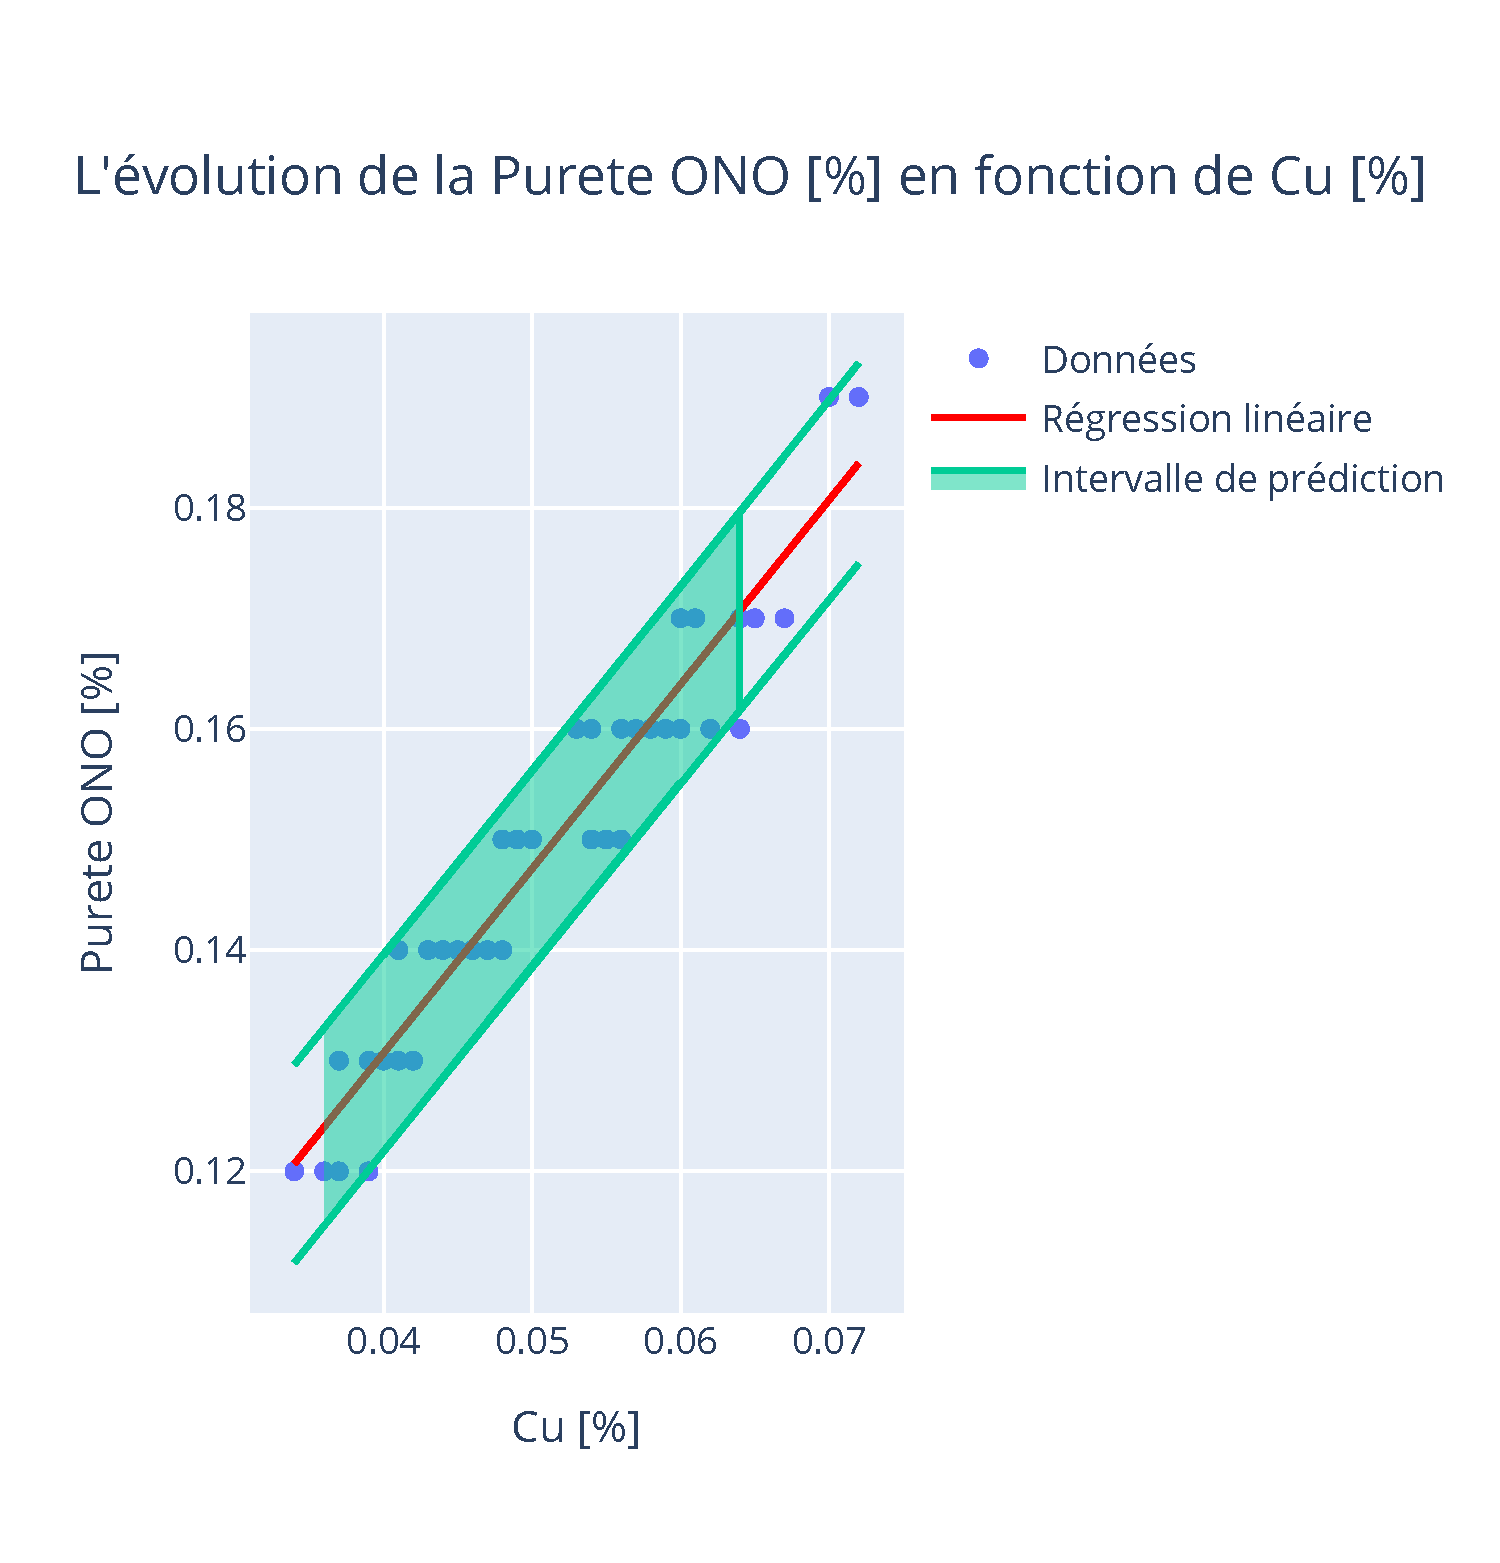
\includegraphics[width=\textwidth]{Images/Statistique/Regression_Ono_Cu.pdf} 
\end{figure}

\textbf{La pureté Ono en fonction du chrome (Cr)} 
\begin{figure}[H]
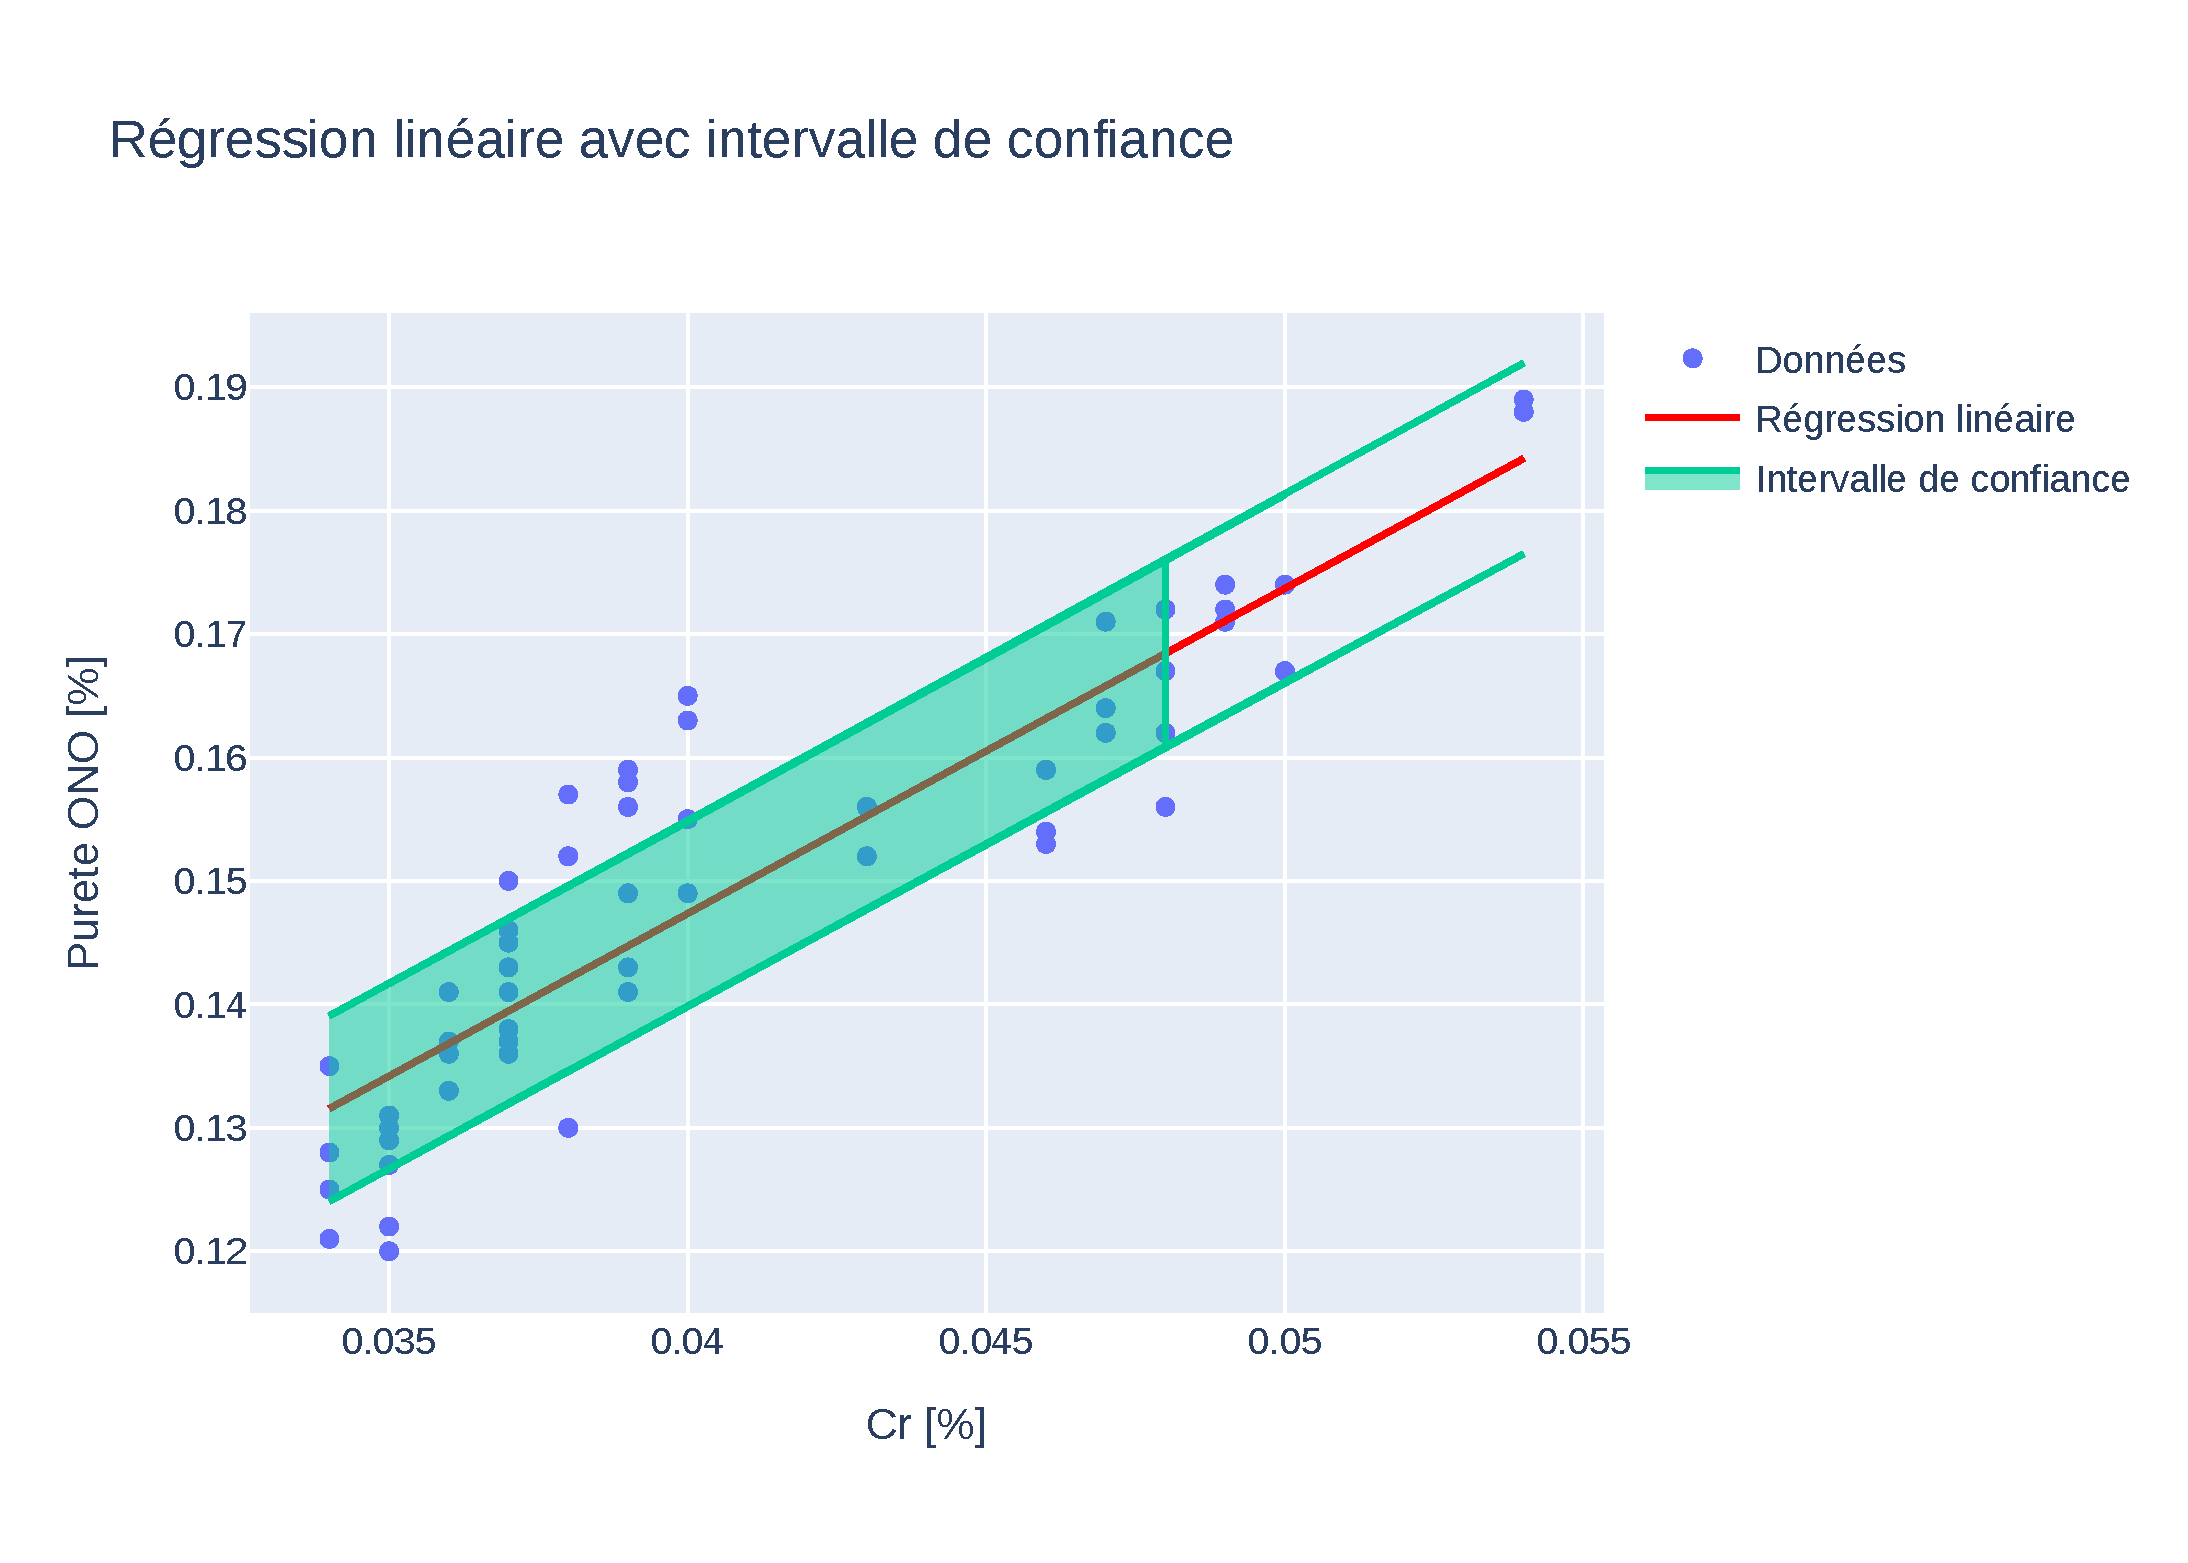
\includegraphics[width=\textwidth]{Images/Statistique/Regression_Ono_Cr.pdf} 
\end{figure}



% Ferrite
\textbf{La Ferrite en fonction du cuivre (Cu)} 
\begin{figure}[H]
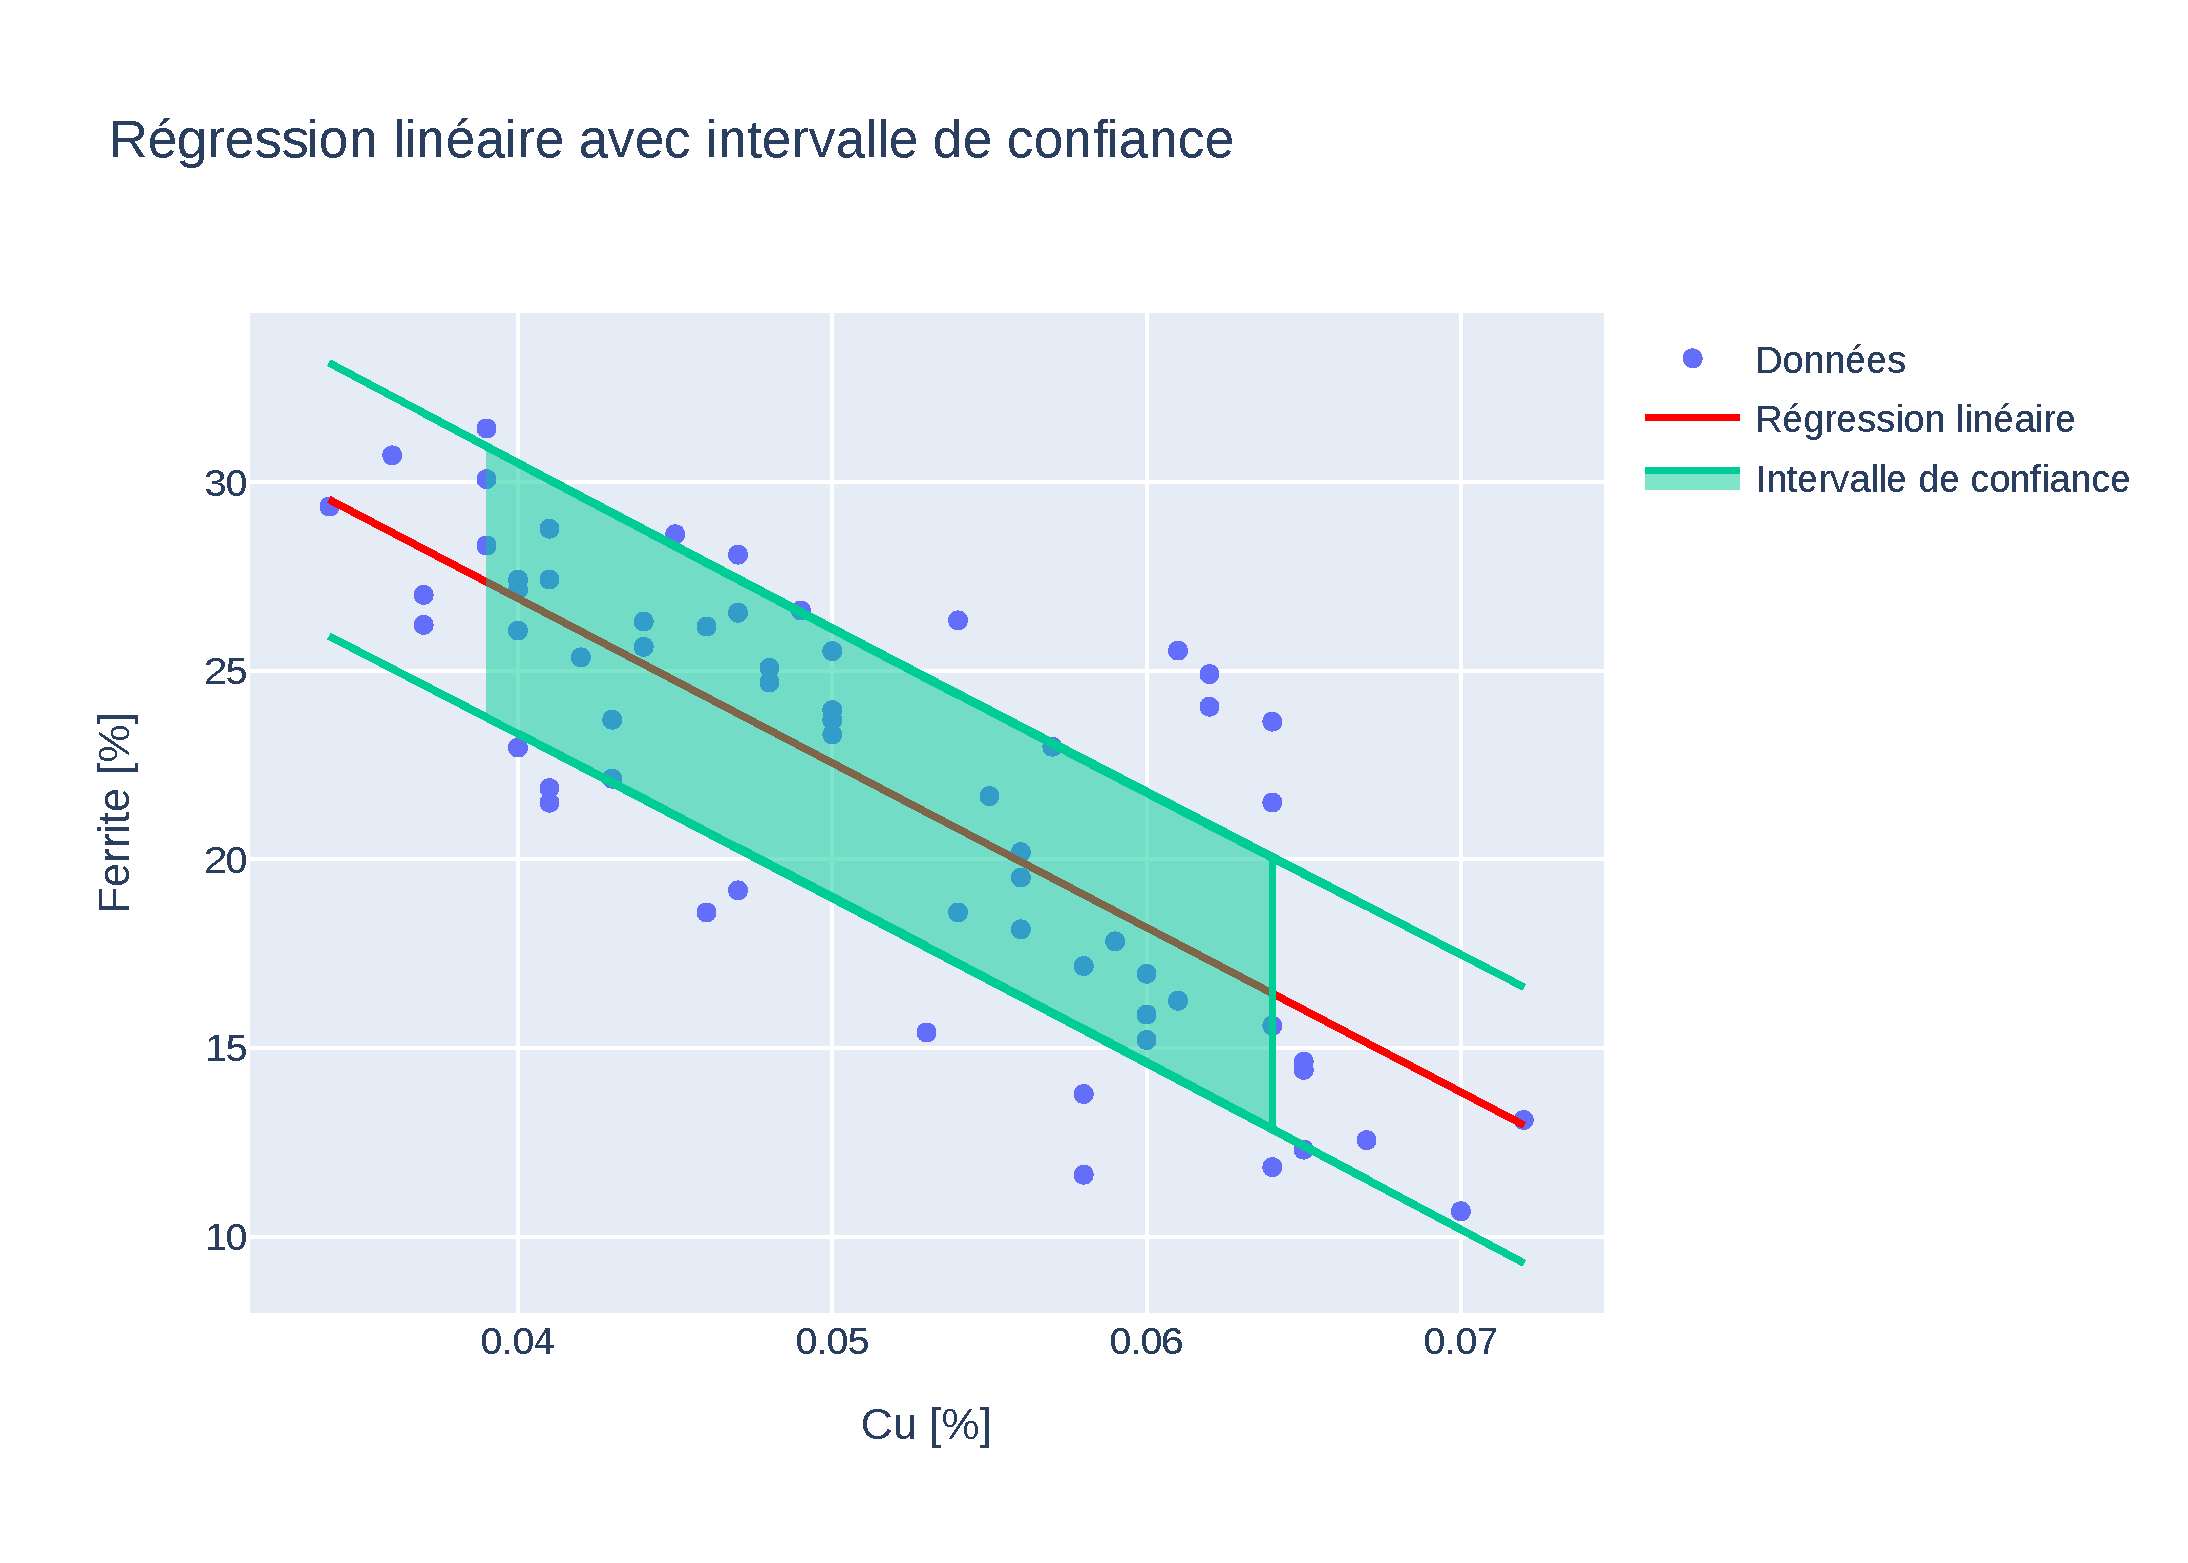
\includegraphics[width=\textwidth]{Images/Statistique/Regression_Ferrite_Cu.pdf} 
\end{figure}


\textbf{La Ferrite en fonction de l'ntimoine Sb} 
\begin{figure}[H]
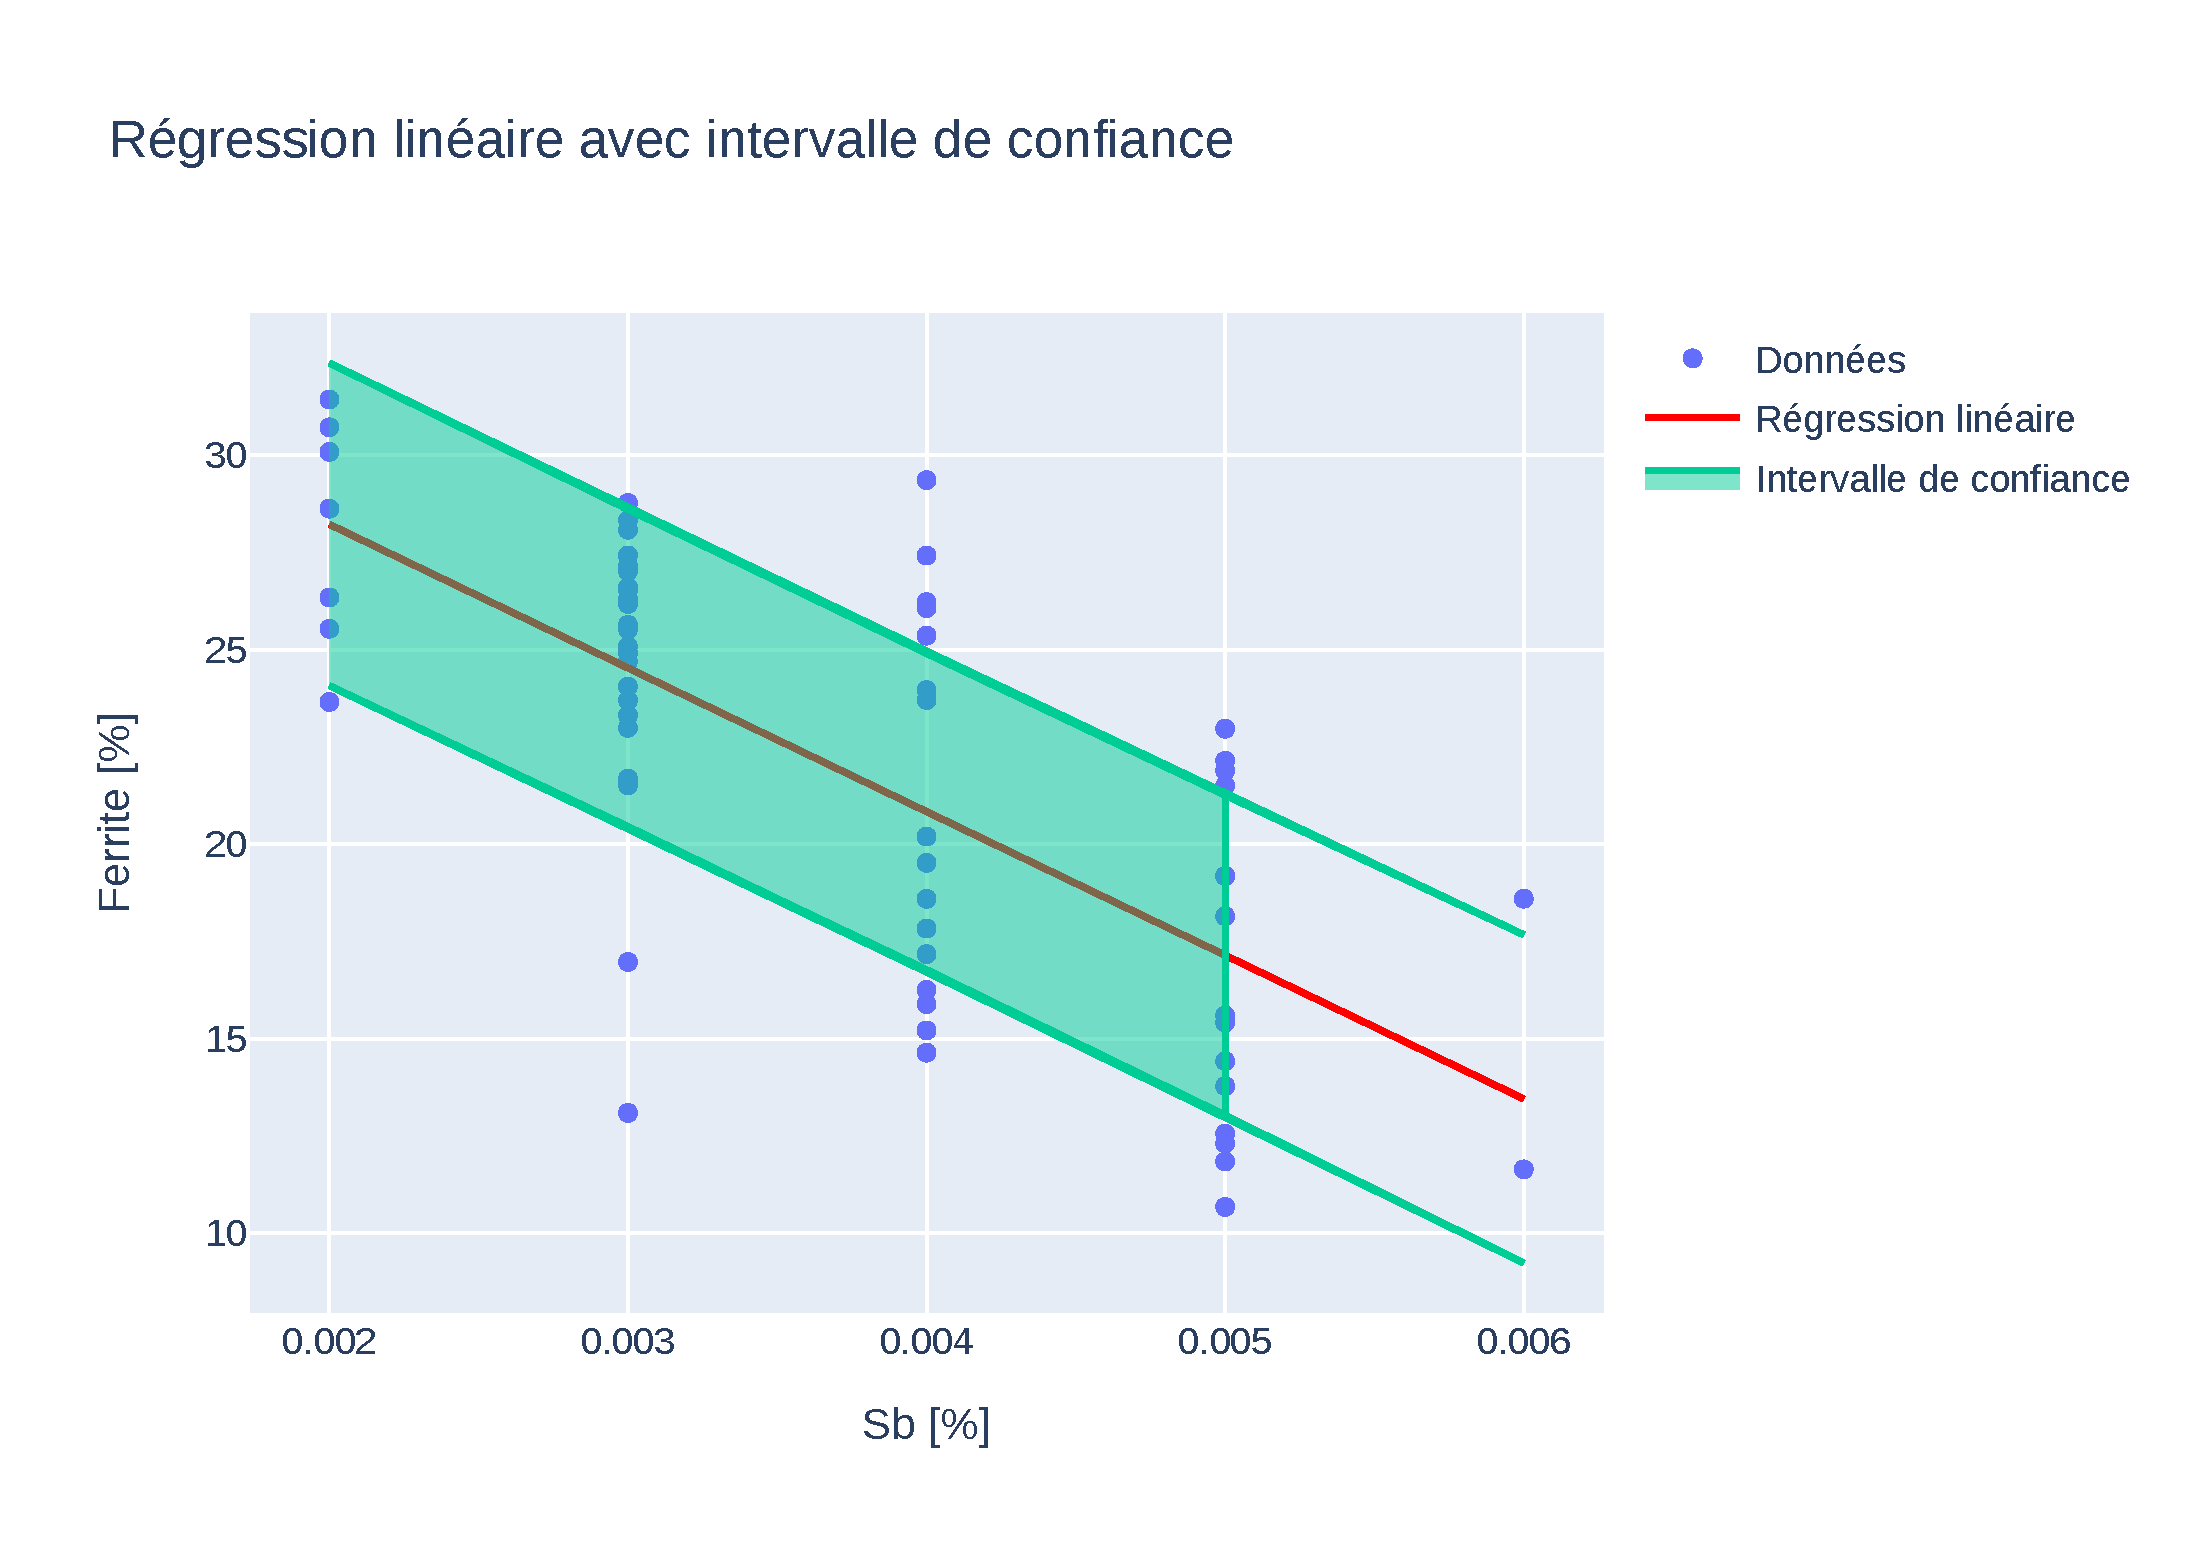
\includegraphics[width=\textwidth]{Images/Statistique/Regression_Ferrite_Sb.pdf} 
\end{figure}




% Rm

\textbf{La Résistance mécanique en fonction du Cuivre} 
\begin{figure}[H]
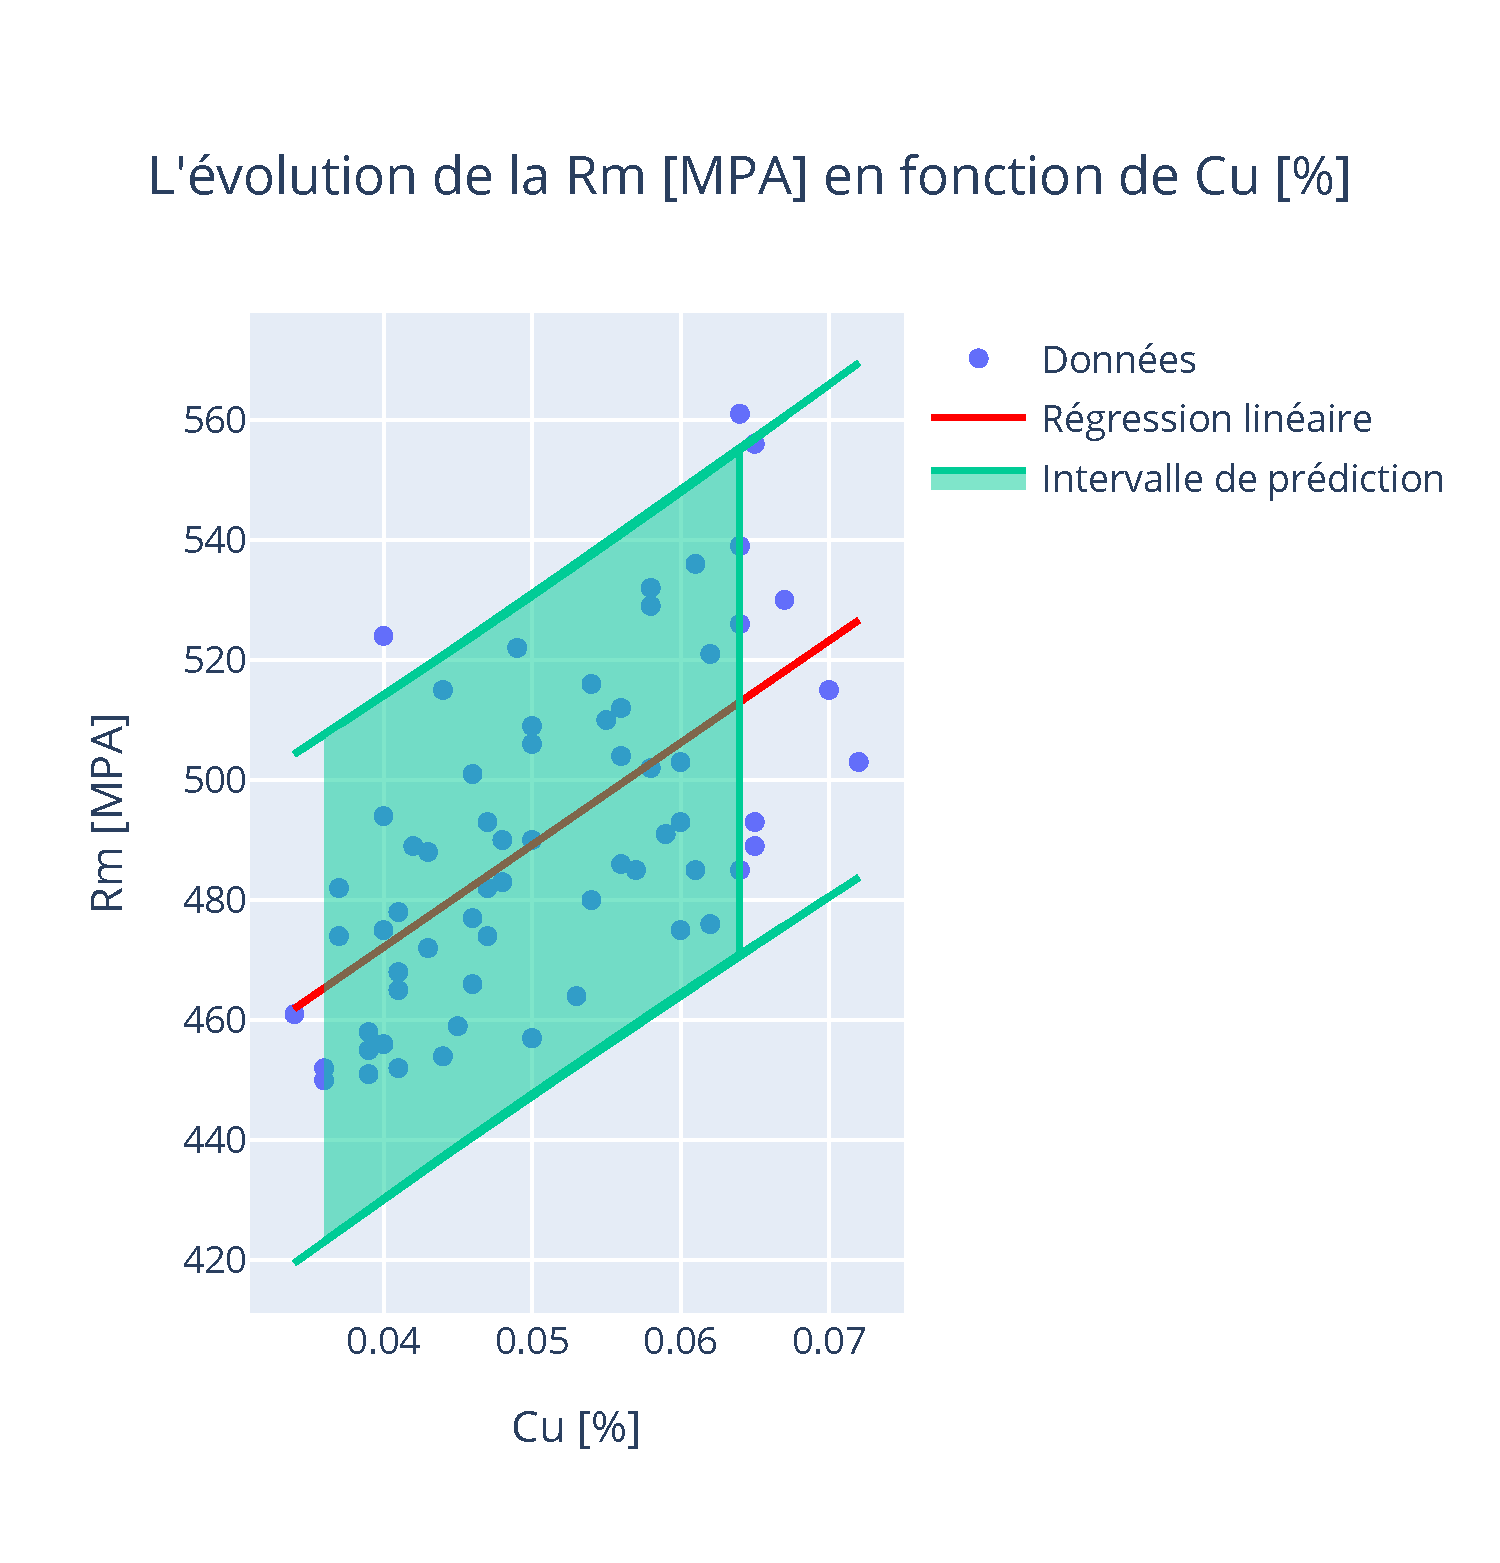
\includegraphics[width=\textwidth]{Images/Statistique/Regression_Cu_Rm.pdf} 
\end{figure}

\textbf{La Résistance mécanique en fonction du Sn} 
\begin{figure}[H]
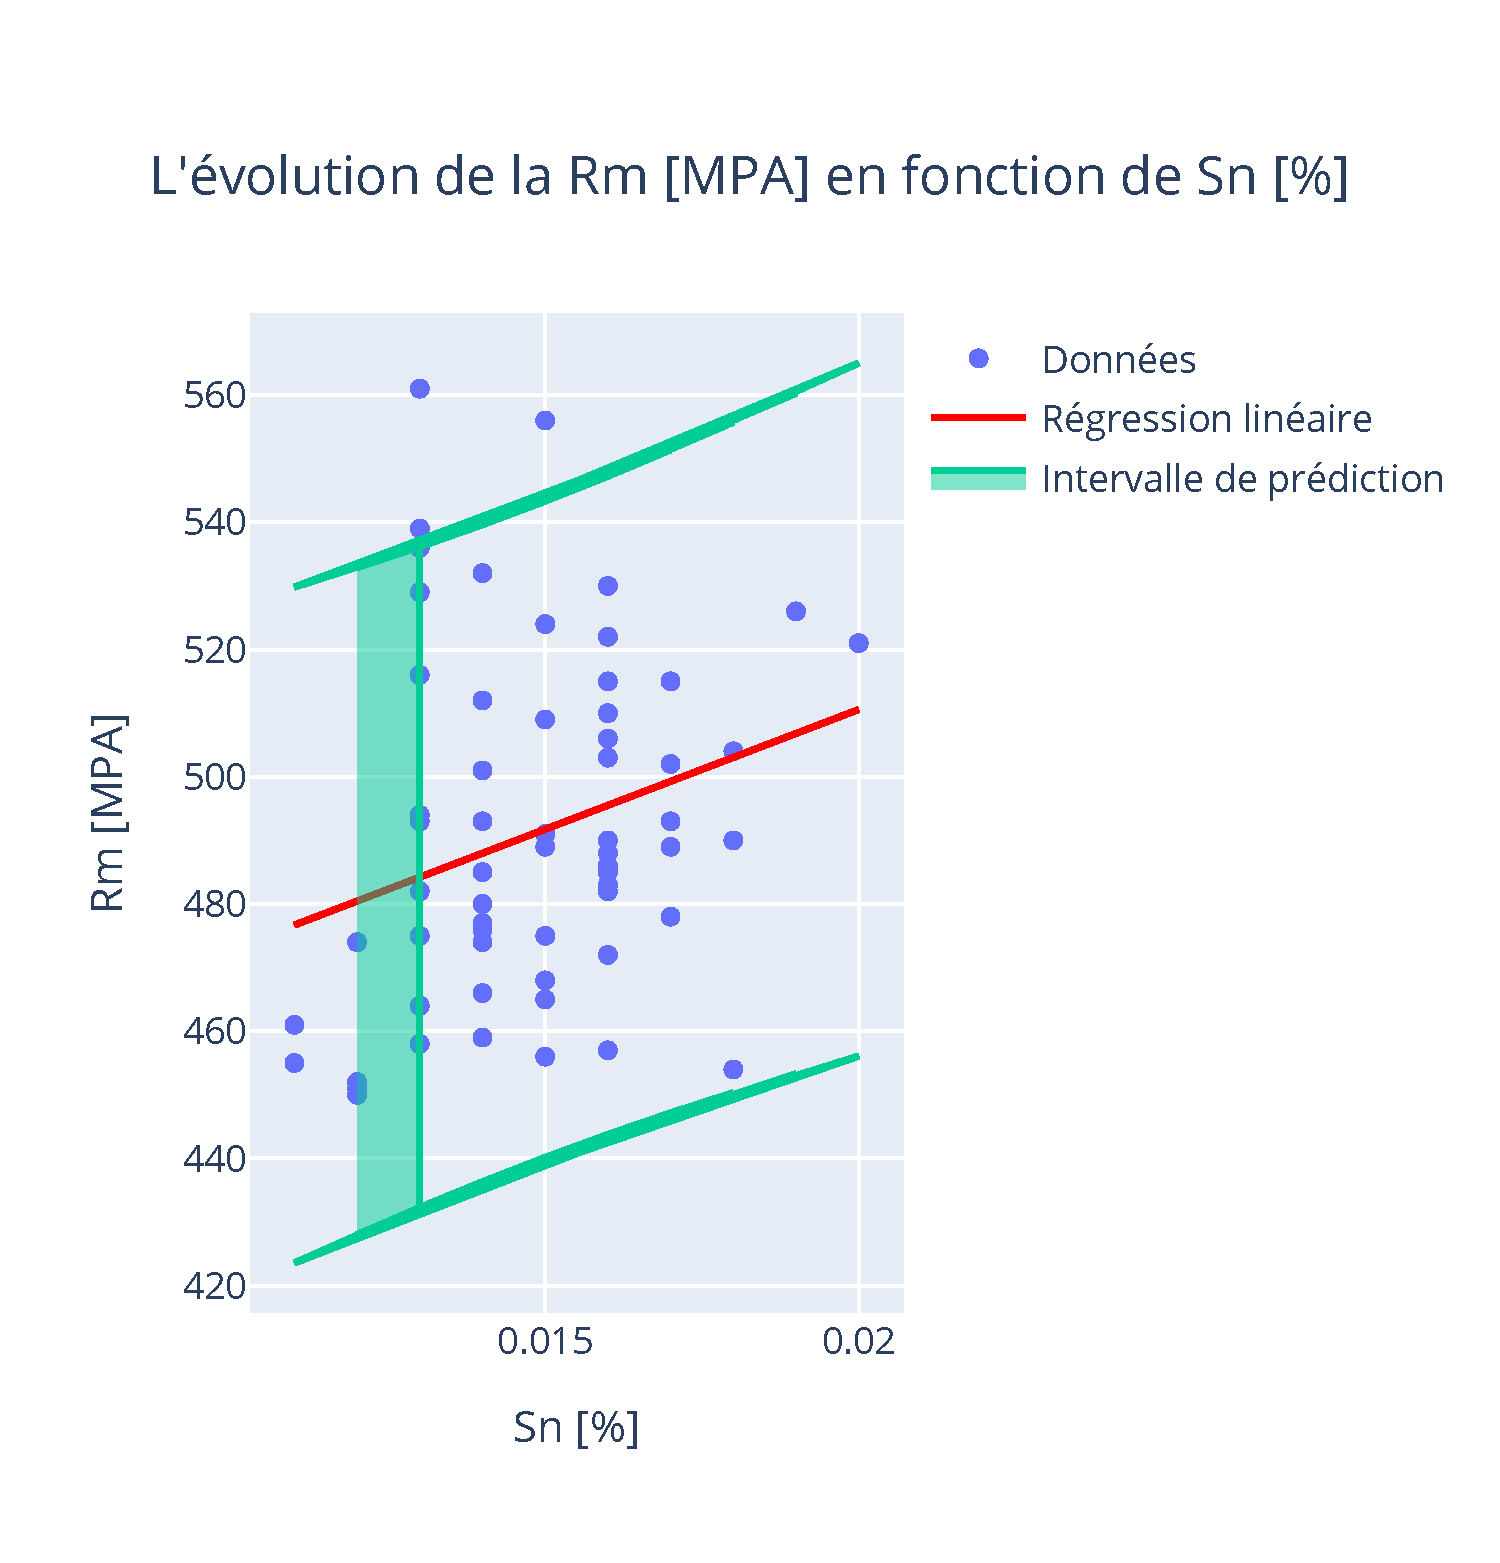
\includegraphics[width=\textwidth]{Images/Statistique/Regression_Sn_Rm.pdf} 
\end{figure}


% Allongement et Rm

\textbf{La Résistance mécanique en fonction du Cr} 
\begin{figure}[H]
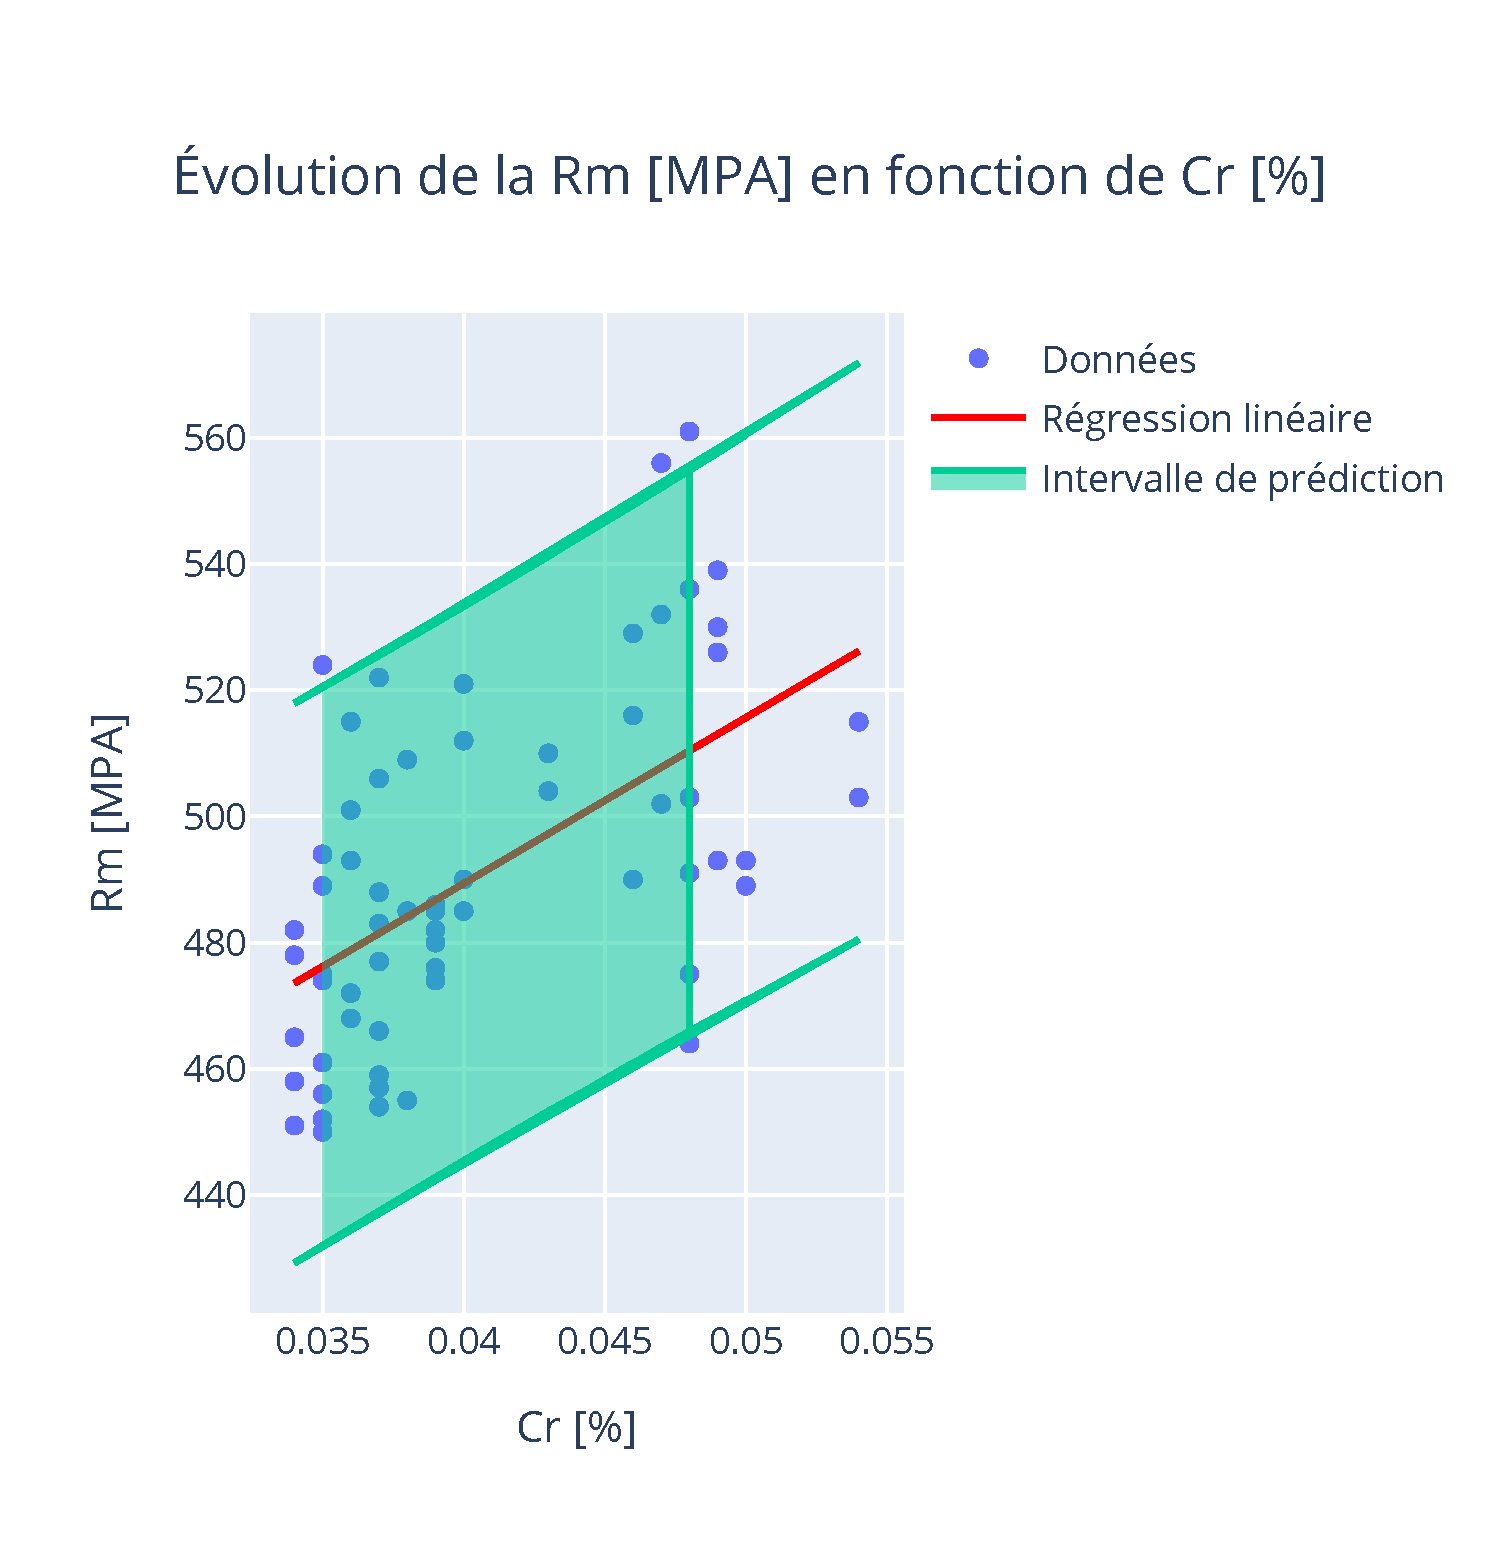
\includegraphics[width=\textwidth]{Images/Statistique/Regression_Cr_Rm.pdf} 
\end{figure}


\textbf{L'allongement en fonction du  Cr} 
\begin{figure}[H]
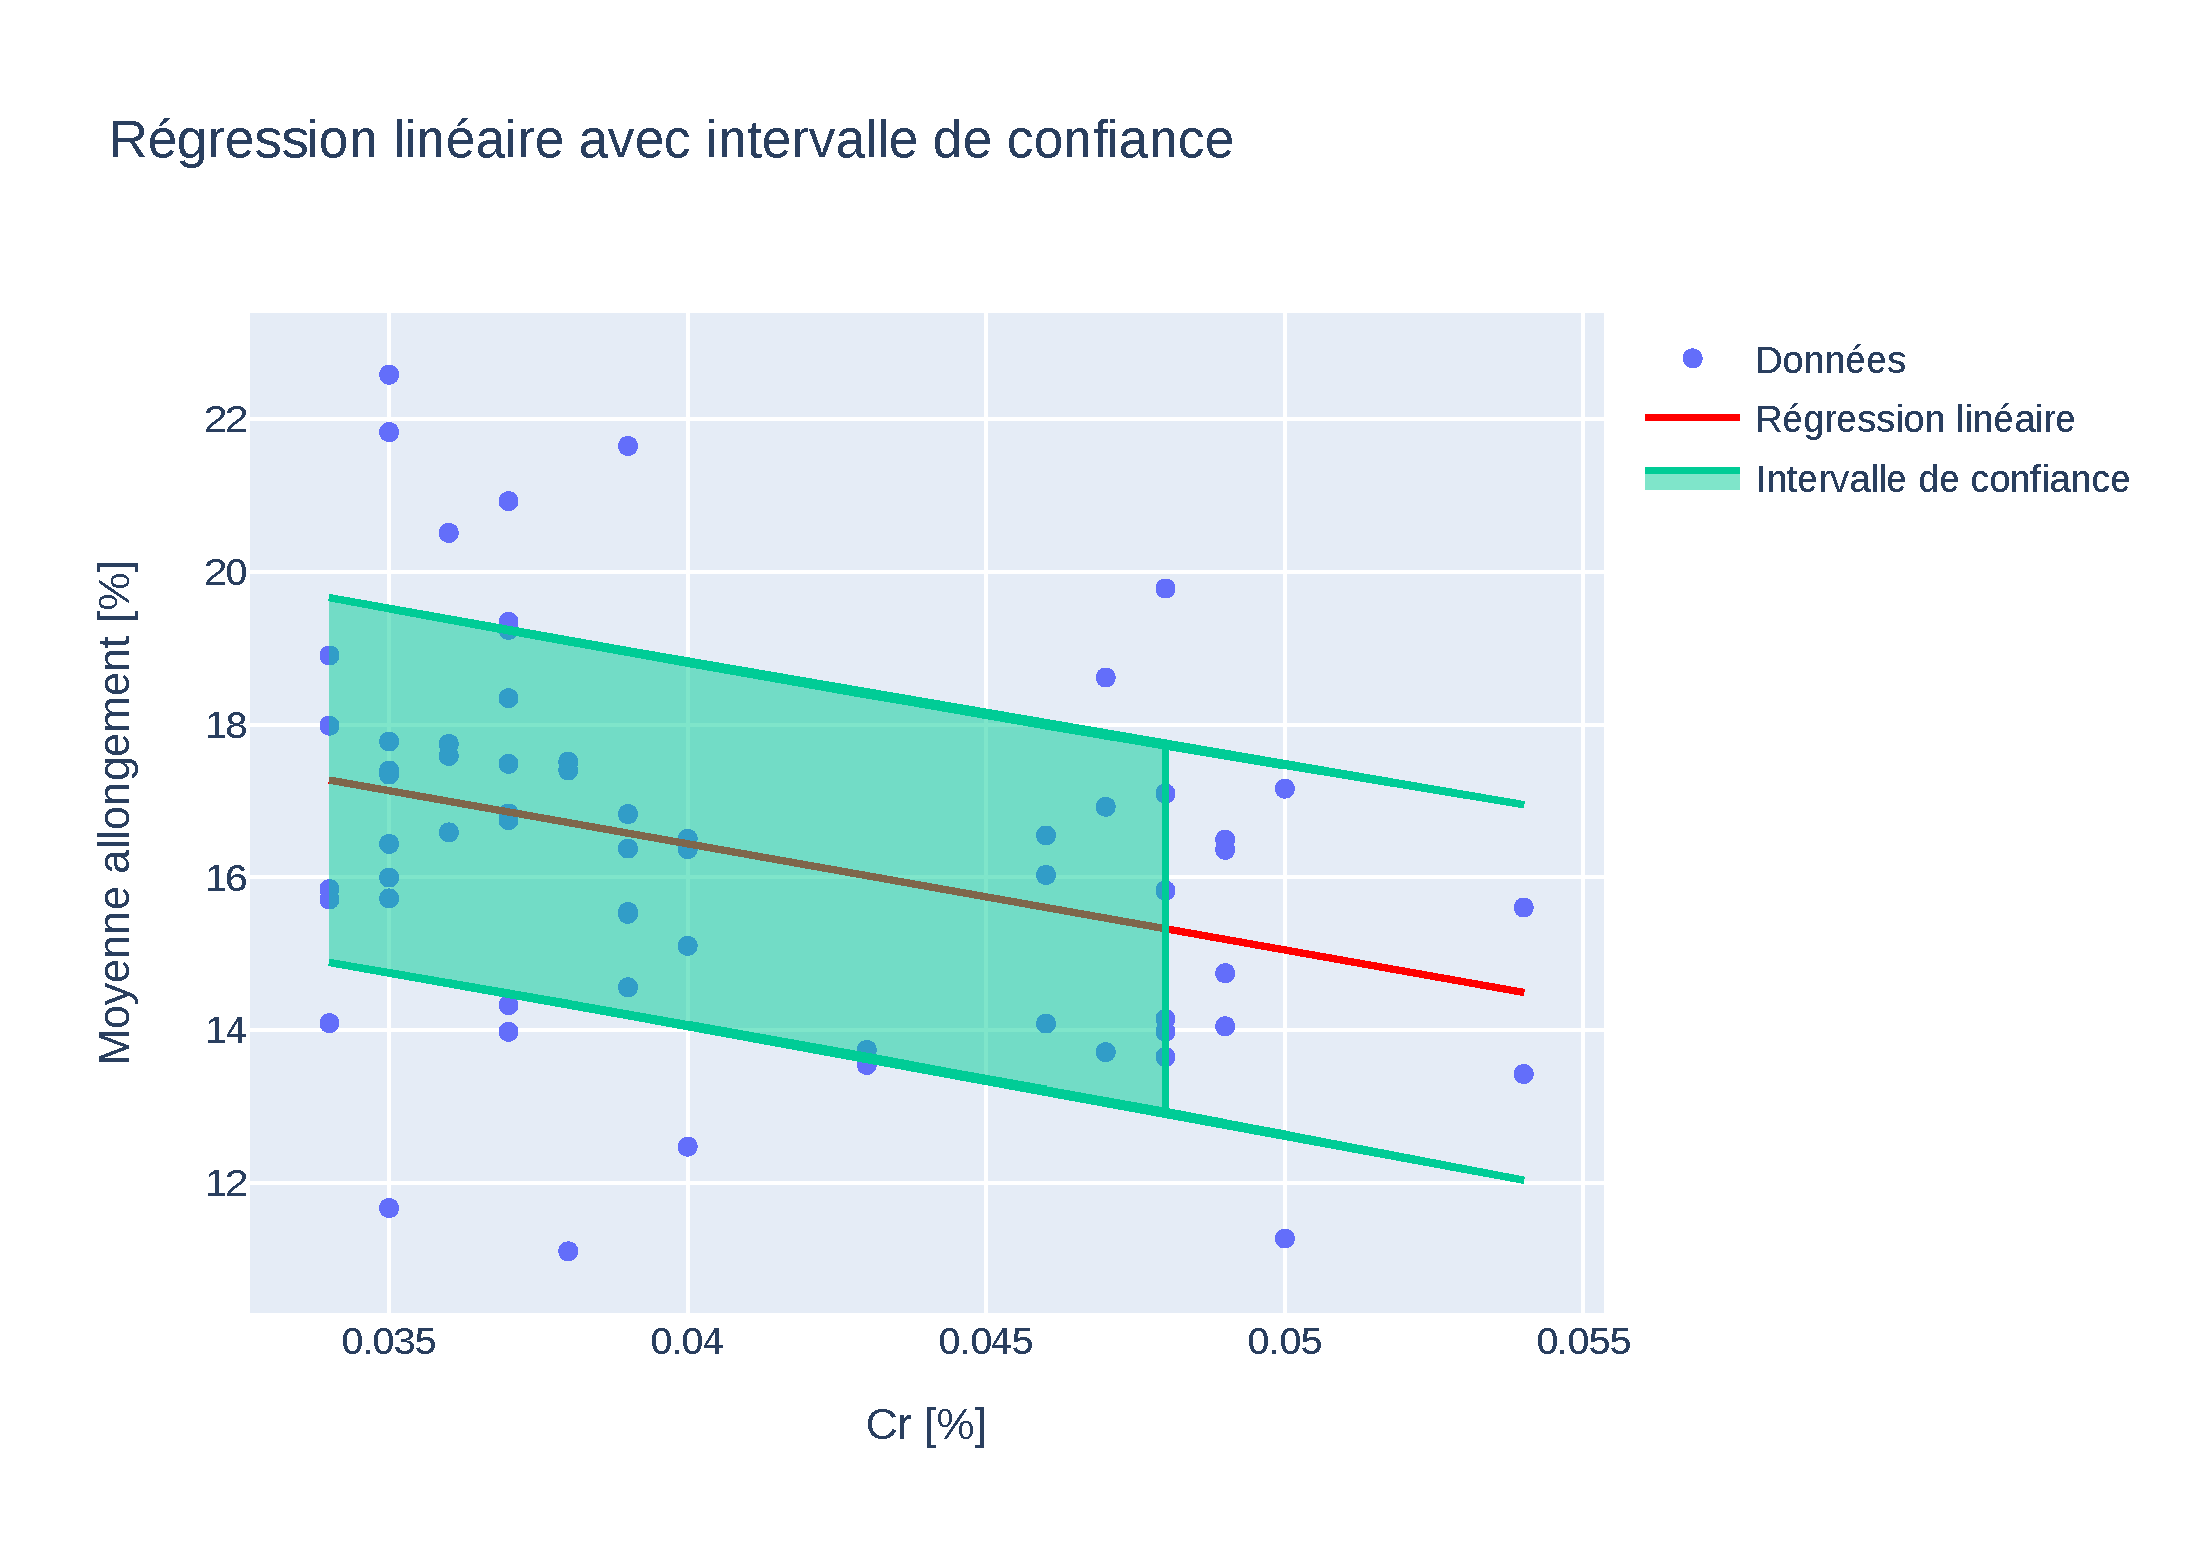
\includegraphics[width=\textwidth]{Images/Statistique/Regression_Cr_Allongement.pdf} 
\end{figure}



% Allongement

\textbf{L'allongement en fonction du Cuivre} 
\begin{figure}[H]
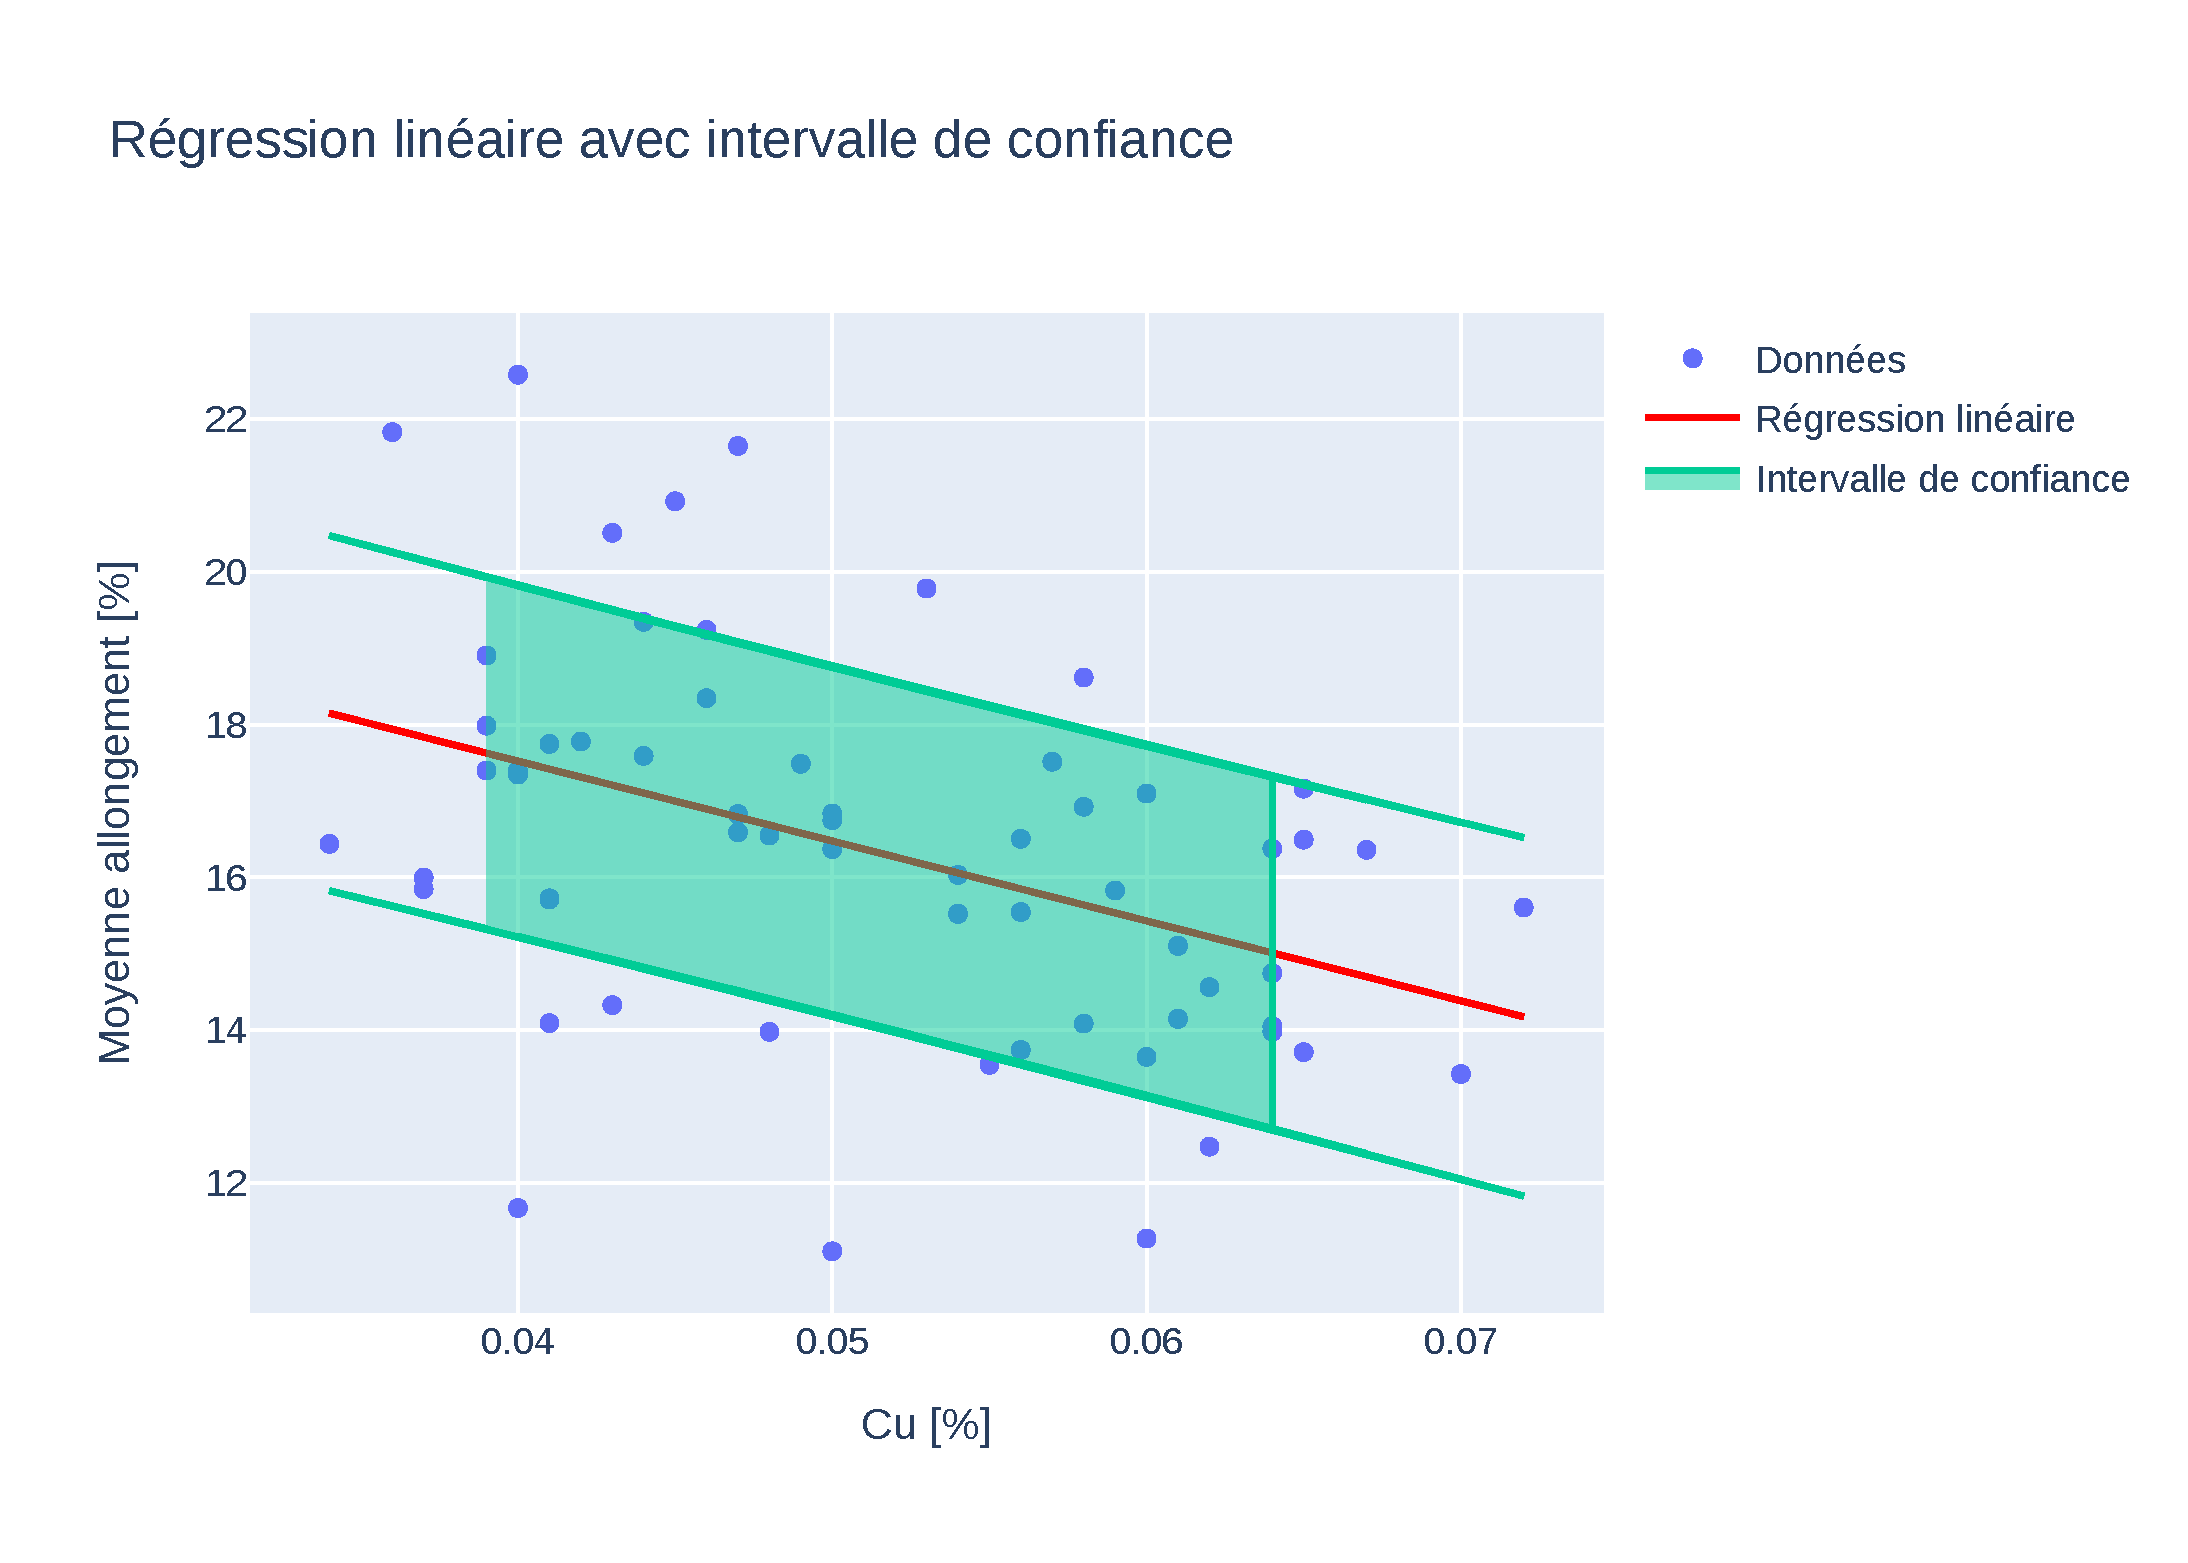
\includegraphics[width=\textwidth]{Images/Statistique/Regression_Cu_Allongement.pdf} 
\end{figure}


\textbf{L'allongement en fonction du Sn}
\begin{figure}[H]
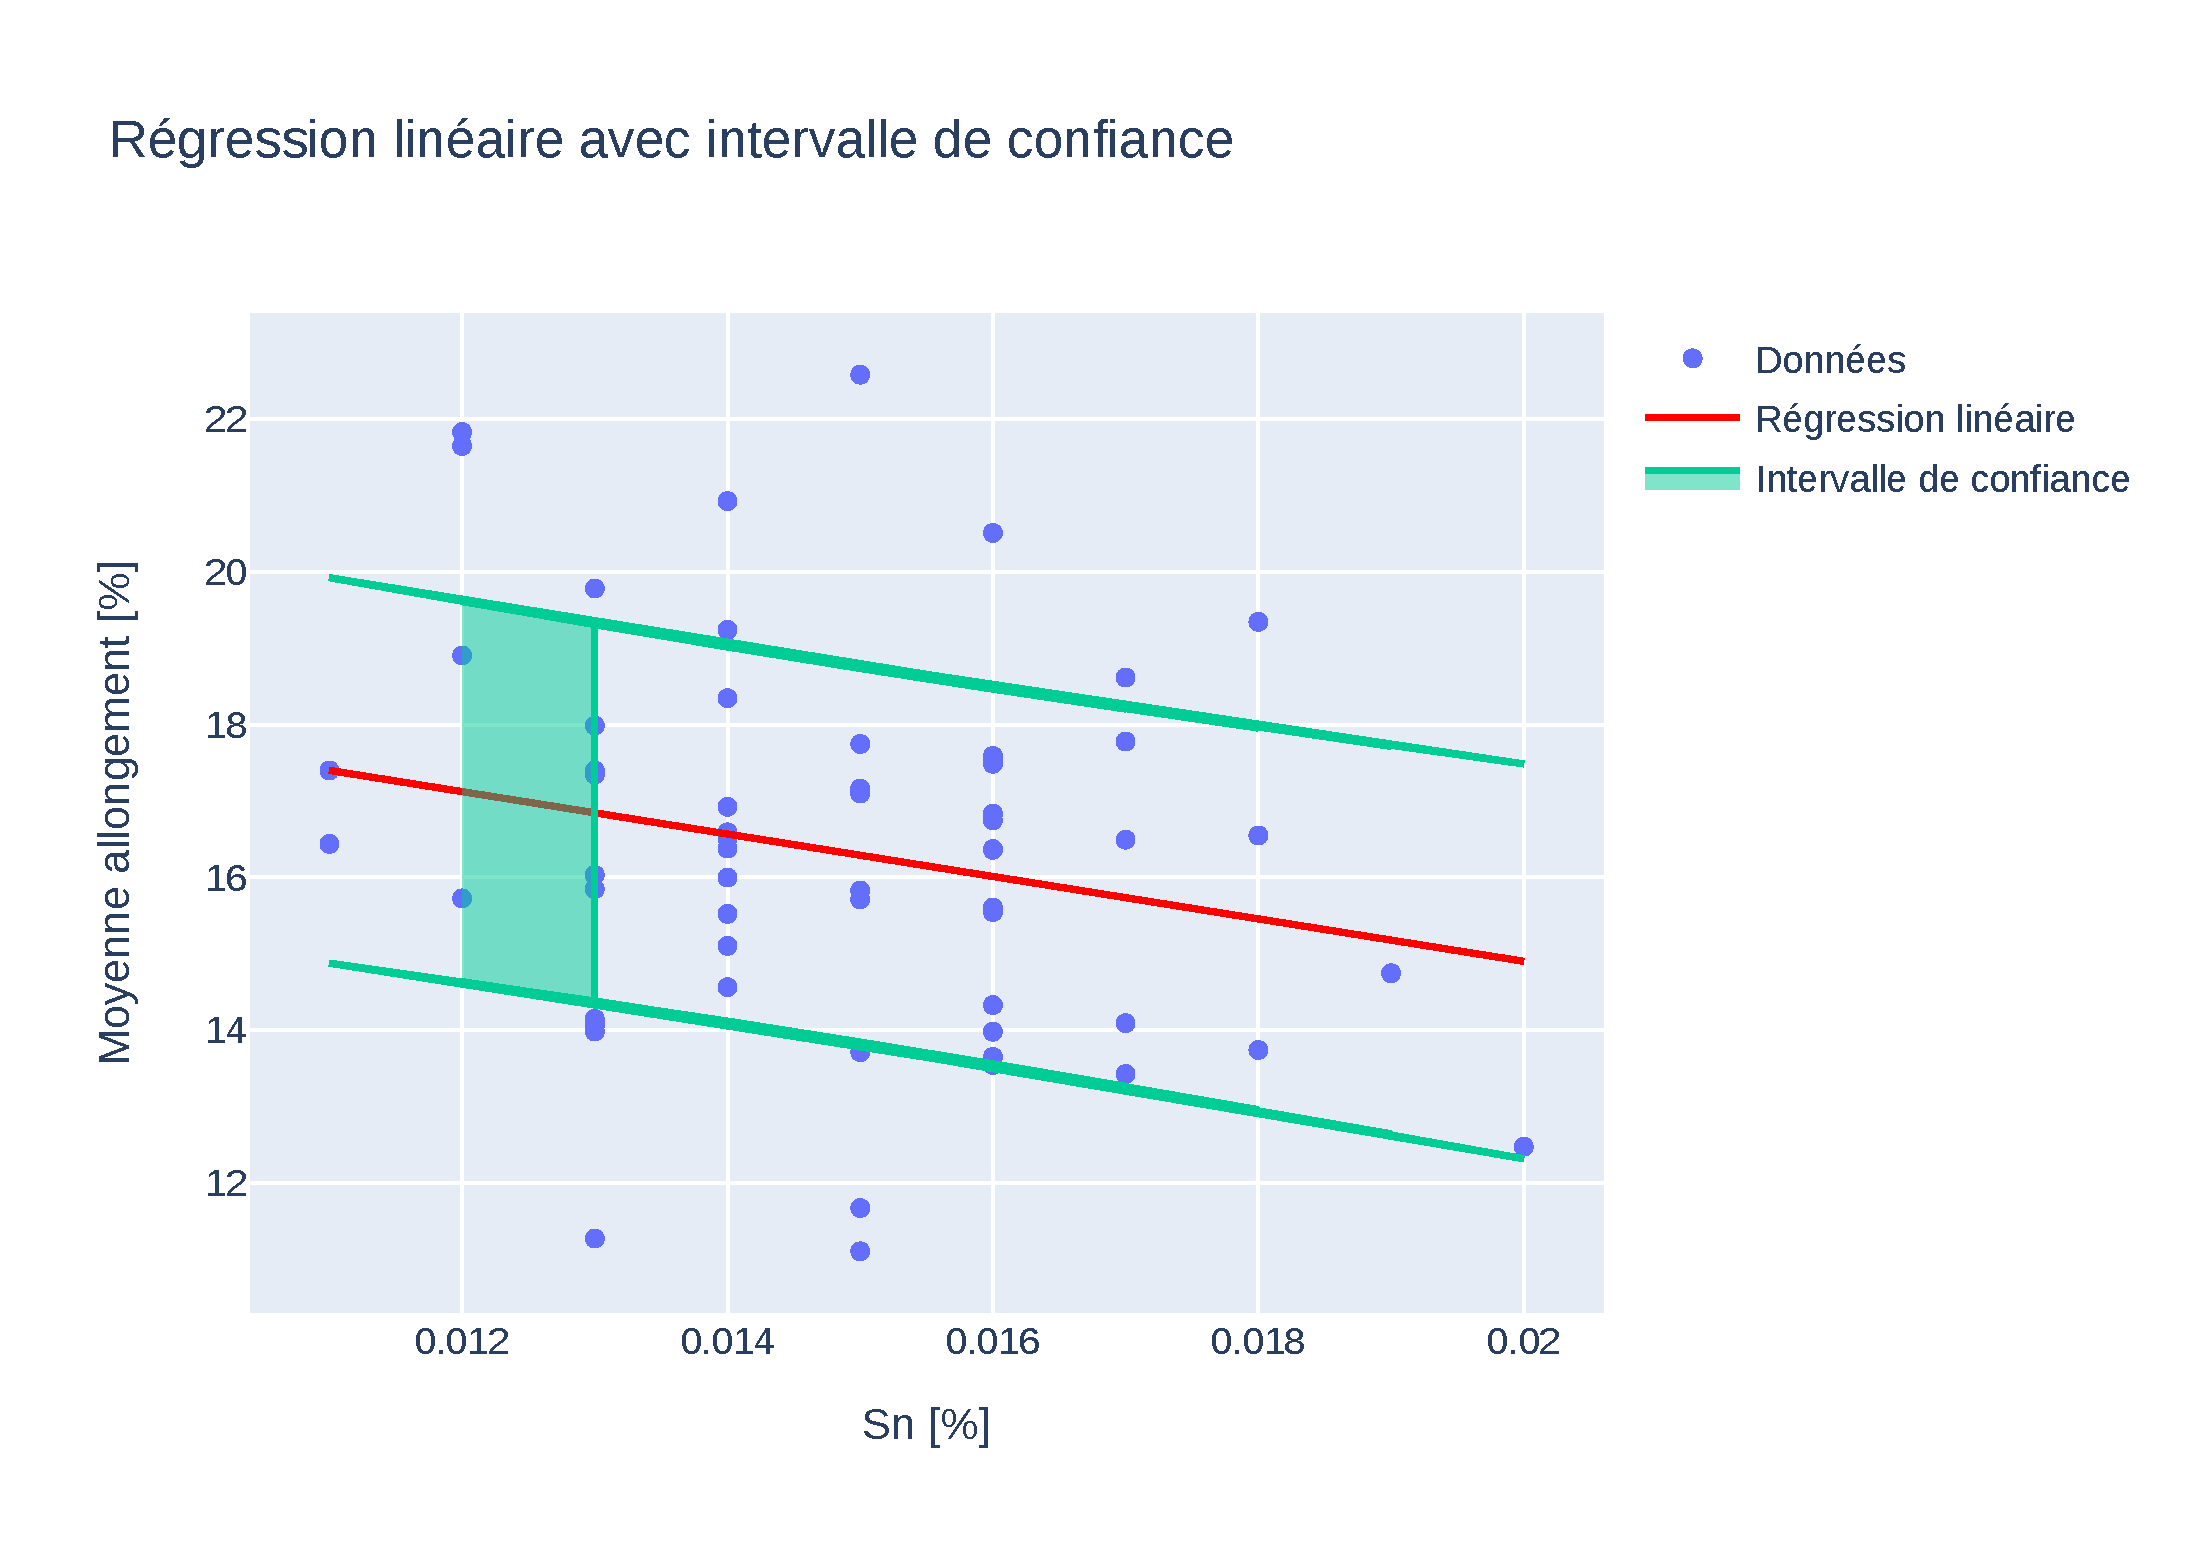
\includegraphics[width=\textwidth]{Images/Statistique/Regression_Sn_Allongement.pdf} 
\end{figure}





\subsection{Conclusion}


% Conclusion 

Nous constatons une corrélation linéaire entre le cuivre et la résistance mécanique, ainsi qu'entre le cuivre et l'allongement. En revanche, pour les autres éléments, la linéarité n'est pas  évidente.



\textbf{Intervalles de confiance des indicateurs :}
\begin{itemize}
\item Impureté : [1.13, 1.19]
\item Pureté ONO : [0.145, 0.153]
\end{itemize}

\textbf{Intervalles de confiance des éléments chimiques :}
\begin{itemize}
\item Sn (Étain) : [0.0143, 0.0153]
\item Cu (Cuivre) : [0.0488, 0.0538]
\item Cr (Chrome) : [0.0392, 0.0422]
\item V (Vanadium) : [0.00092, 0.00111]
\end{itemize}


















\section{La recette Optimale}

\subsection{Présentation du problème d'Optimisation }

Dans le cadre du processus de fabrication de 5 tonnes de fontes, l'une des étapes préliminaires fondamentales
réside dans la détermination du lit de fusion, c'est-à-dire la proportion des matières premières
nécessaires à la fusion. Dans notre cas, on souhaite  produire une tonne de fonte de haute qualité.
Pour ce faire, nous disposons d'une trentaine de matières premières, chacune possédant sa propre
composition chimique distinctive. Chaque matière première est disponible ou non en quantité limitée
et leurs prix varient tout au long de l'année. Ces matières sont issues de diverses sources,
comprenant des matériaux métalliques et de construction, ainsi que des retours, c'est-à-dire
des résidus provenant des précédents cycles de production. Par exemple, parmi ces matériaux,
on trouve les SABOTS DE FREINS SNCF, les RAILS DE CHEMIN DE FER de 40 cm et de la FONTE GS RECYCLÉE,
dont les prix respectifs sont de 435 euros, 423,90 euros et 374 euros. La qualité de la fonte dépend
de sa composition chimique, qui doit se situer dans des intervalles spécifiques adaptés au type
de fonte recherché, tout en respectant des critères de qualité tels que le niveau d'impuretés et
la pureté ONO. Le niveau d'impuretés et la pureté ONO sont déterminés par des combinaisons linéaires
des pourcentages d'éléments chimiques présents dans les matières premières. Par conséquent,
l'objectif principal est de déterminer les proportions optimales des matières premières,
en vue de minimiser les coûts de production tout en préservant la qualité de la fonte.

% (Afficher les images de matières premières de la fonderie)

\subsection{Modélisation du problème}



Phase Tansitoire 

- Explication de cette phase 


- Obtention des images inputs, outpouts Optimisation de la Presentations
Dans le drive , exporter en pdf avec parametre Paysage, Statement, dessus puis bas


Les différents étapes  de la poche 1


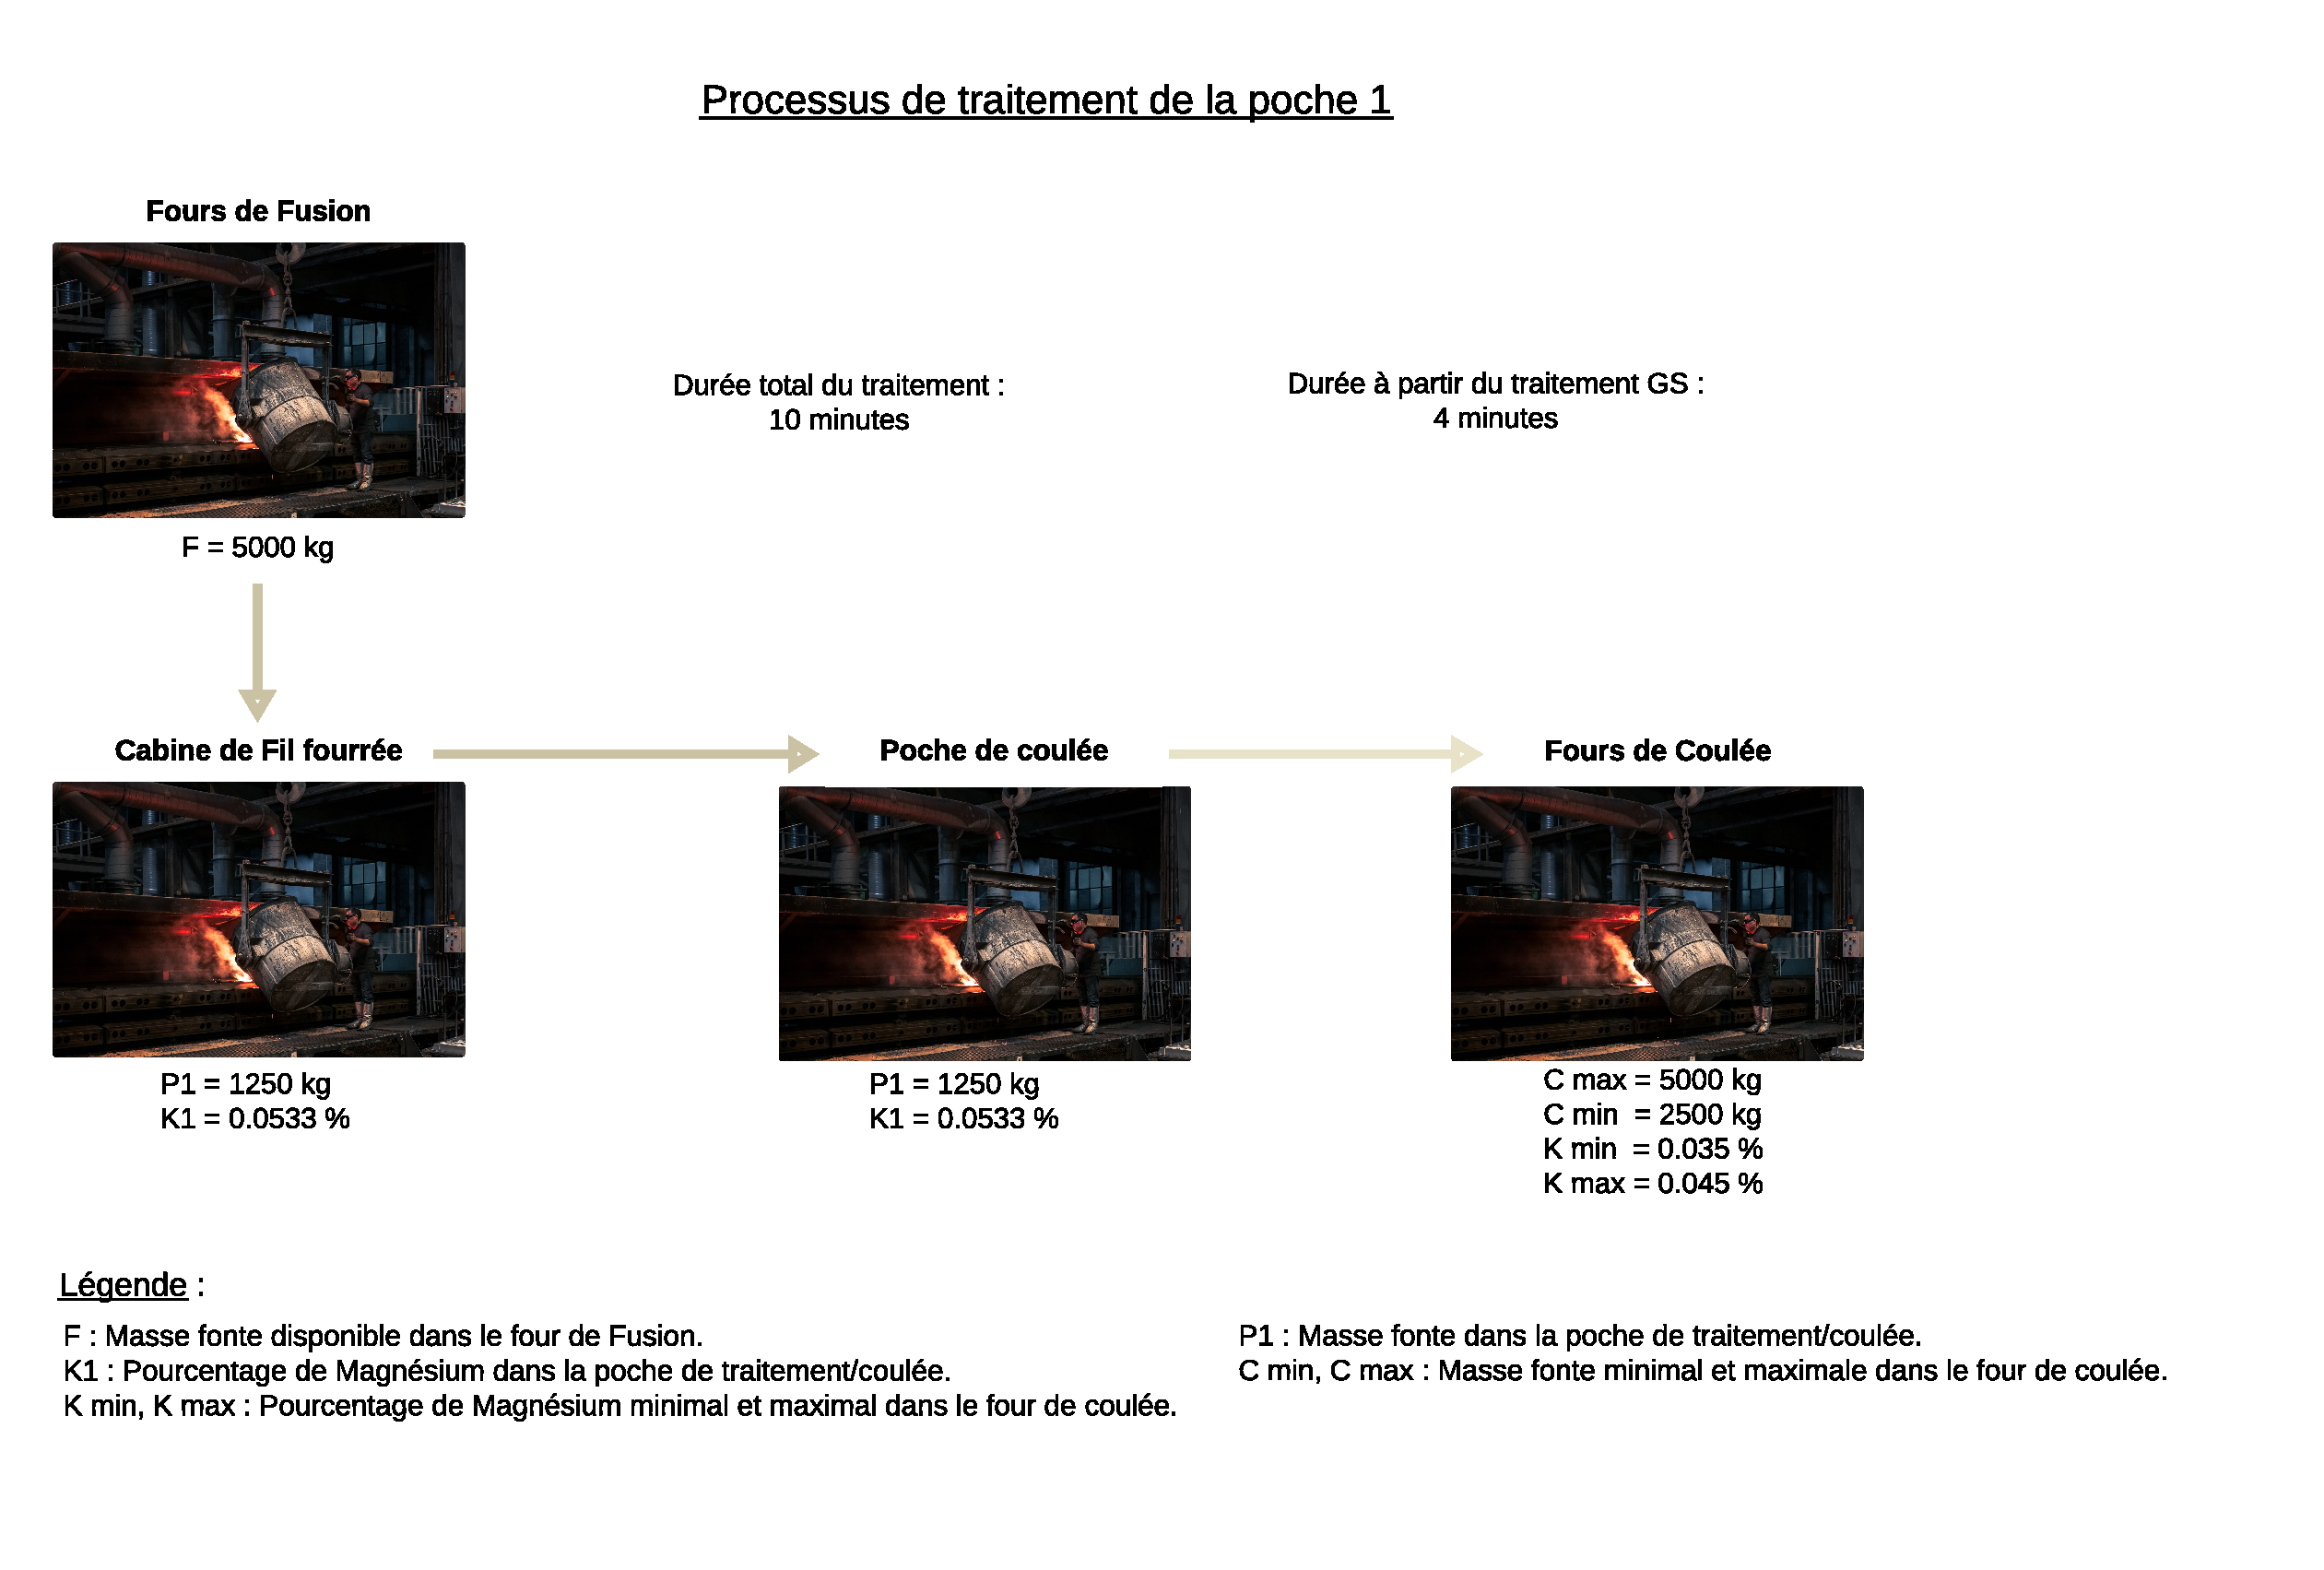
\includepdf[pages=-, scale=1]{Images/Poche 1.pdf}
\includepdf[pages=-, scale=1]{Images/Poche 2.pdf}
\includepdf[pages=-, scale=1]{Images/Poche 3.pdf}



\begin{table}[H]
    \caption{Tableau 1.5: Composition chimique des fontes GS (ADI) [26]}
    \centering
        \begin{tabular}{|c|c|}
        \hline
        Nuance & Carbone [\%] \\ \hline
        GS 400-15 & 3.50-4.00  \\ \hline
        GS 450-10 & 3.50-4.00  \\ \hline
        \end{tabular}
\end{table}
    
    
% \begin{table}[H]
% \caption{Tableau 1.5: composition chimique des fontes GS (ADI) [26]}
%     \begin{tabular}{|l|l|l|l|l|l|l|}
%     \hline
%     Nuance & Carbone (\%) & Silicium (\%) & Manganèse (\%) & Phosphore (\%) & Soufre (\%) & Magnésium (\%) & Cuivre (\%) \\ \hline
%     FGS400-15 & 3.50-4.00 & 2.50-2.80 & <0.30 & 4.30-4.95 & <0.06 & <0.20 \\ \hline
%     FGS450-10 & 3.50-4.00 & 2.50-2.88 & <0.45 & 4.30-4.90 & <0.06 & <0.20 \\ \hline
%     \end{tabular}
% \end{table}

\subsection{La méthode du simplexe}

\subsection{Mise en oeuvre de la méthode du simplexe}

LE prix du fil Fourre en metre est de ...


\begin{thebibliography}{9}

\bibitem{Gianluigi Rozza}
Gianluigi Rozza.  \emph{An introduction to reduced basis method for parametrized PDEs, ResearchGate}

\bibitem{B. Haasdonk}
B. Haasdonk.  \emph{Reduced Basis Methods for Parametrized PDEs –
A Tutorial Introduction for Stationary and
Instationary Problems, University of Stuttgart  } 


\bibitem{Alexandre Ern}

\bibitem{Bopeng RAO}
Bopeng RAO,  \emph{ Méthodes Numériques
des Equations aux Dérivées Partielles. UFR de Mathématique et d’Informatique
Université de Strasbourg, 2021-2022 }

\bibitem{Gwenol Grandperrin}
Gwenol Grandperrin.  \emph{Introduction à la méthode des bases réduites, ResearchGate Janvier 2008 }

\end{thebibliography}

\end{document}